\section{Realisierung}
\label{sec:realisierung}

Die Entwicklung eines eigenen Simulationstools war nicht vorgesehen.
Für die Simulationsläufe wurde die Abwandlung einer Software verwendet, die als \enquote{Traffic Simulation Game} für einen Workshop mit Doktoranden\footnote{\url{https://lightjason.github.io/news/2017-09-workshop/}} erstellt worden war.

In diesem Workshop mussten die Teilnehmer mit Hilfe der Agentensprache ein Fahrzeug steuern. Dieses sollte ein 50 km langes Straßenstück mit unterschiedlichen zufälligen Geschwindigkeitsbegrenzungen zurücklegen. Ziel war es, wenige Verkehrsverstöße zu begehen und dennoch möglichst schnell zu sein.

Für die Zwecke dieser Arbeit musste die Software weiter angepasst werden.
Dabei mussten während der Tests der ersten Agentenpläne Korrekturen vorgenommen werden, da eine fehlerfreie Simulation sonst nicht möglich gewesen wäre. 
Mehr dazu nachfolgend in \cref{sec:anpassungen-probleme}.
Fehlersuche und kleinere Anpassungen wurden selbst geleistet.
Umfangreichere Codeänderungen erfolgten durch den Ersteller des Tools, Philipp Kraus.

%\pk{Kann, darf, soll, muss ich hier darauf hinweisen, dass die Programmierung nicht meine Aufgabe war und dass Du das gemacht hast?}
%\sa{Das musst Du sogar machen, das war aber eine explizite Vorgabe für Deine Arbeit, Du solltest aber auch dazu schreiben, dass Du eben einige Anpassungen gemacht hast, da es nicht richtig funktioniert hat}



\subsection{Entwicklung des Agentenverhaltens}%\sa{mit dem Kapitel beginnen und dann auf die Umwelt eingehen -> klar durch strukturieren, Du redest vorher schon von Agent, aber wie der jetzt bei Dir zum Nutzen kommt ist bis zu diesem Kapitel für den Leser nicht klar}
\label{sec:entwicklung-agentenplan}

Jeder Agent in den Simulationen, die dieser Arbeit zugrunde liegen, stellt ein individuelles Fahrzeug dar.
Die mathematischen Gleichungen in \cite{na-sch} beschreiben gut, welches Verhalten dem Agenten zu geben ist: 
\begin{itemize}
\itemsep0em
	\item wenn möglich beschleunigen
	\item zufällige Reduktion der Geschwindigkeit (Trödeln)
	\item wenn nötig abbremsen
\end{itemize}


\subsubsection{Zustandsautomat}

Das oben beschriebene Verhalten wurde zuerst mit Hilfe eines endlichen Automaten beschrieben, siehe \cref{figure:fsm-nasch}.

\begin{figure}[hptb]
 \centering
 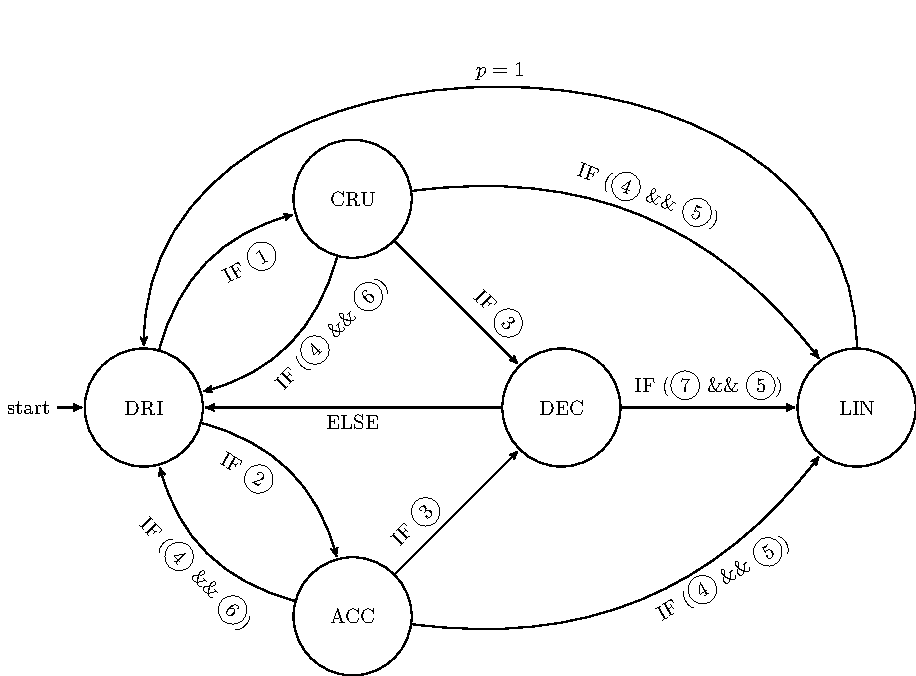
\includegraphics[width=0.9\textwidth]{fsm-nasch}
 \caption[Zustandsautomat für das Agentenverhalten]
 		{Zustandsautomat für das Agentenverhalten nach dem Nagel-Schreckenberg-Modell}
 \label{figure:fsm-nasch}
\end{figure}

\noindent
Erläuterungen zu \cref{figure:fsm-nasch}:
\begin{enumerate}
\itemsep0em
	\item  $ v_{aktuell}  \leq  v_{limit} $
	\item  $ v_{aktuell}  <  v_{limit} $
	\item  \enquote{Verkehr voraus}
	\item  \enquote{kein Verkehr voraus} \texttt{UND} $ p_{linger} $
	\item  \enquote{kein Verkehr voraus} \texttt{UND} $ 1 - p_{linger} $
	\item  $ v_{aktuell}  > 0 $ \texttt{UND} $ p_{linger} $
\end{enumerate}

Startzustand des Automaten ist ein allgemeiner Zustand \texttt{DRI} (Drive/Fahren), in dem nichts am Verhalten des Agenten geändert wird.
Von hier aus ist der Zustand \texttt{ACC} (Accelerate/Beschleunigen) zu erreichen, wenn die aktuelle Geschwindigkeit unter der max. zulässigen liegt. 
Der Zustand \texttt{CRU} (Cruisen) wird erreicht, wenn die max. zulässige Geschwindigkeit erreicht oder überschritten ist.

Die Übergänge aus den zwei letztgenannten Zuständen sind identisch. 
Ist kein vorausfahrender Verkehr vorhanden und wird nicht getrödelt erfolgt der Übergang zurück in den normalen \texttt{DRI}-Zustand.
Wird stattdessen zufällig mit Wahrscheinlichkeit $ p_{linger} $ das Trödeln angestoßen, wird der entsprechende Zustand \texttt{LIN} erreicht.
Ist Verkehr voraus, wird der Zustand \texttt{DEC} (Decelerate/Verzögern, Bremsen) erreicht.

Aus dem \texttt{DEC}-Zustand kann zufällig ein Übergang in den \texttt{LIN}-Zustand erfolgen ansonsten zurück in den allgemeinen \texttt{DRI}-Zustand.
Aus dem \texttt{LIN}-Zustand wird zwangsläufig wieder in den \texttt{DRI}-Zustand übergegangen.

Ein Zeitschritt der Simulation entspricht dabei einem Zyklus vom Startzustand ausgehend bis zur Rückkehr dorthin.


\subsubsection{Agentenpläne}

Der o.g. Automat wurde in die Agentensprache \enquote{übersetzt}. 
Die Agentenversion unterscheidet sich dabei leicht von der Automatenversion. 

Der Agent beginnt im Plan \texttt{cruise}, von dem aus alle weiteren Pläne (\texttt{accelerate}, \texttt{linger}, \texttt{decelerate}) gestartet werden.
Außerdem ruft sich der Plan selbst wieder auf.
\\
Während der Simulationsläufe diente dieser Plan zudem dem Loggen der Statusdaten.
Das komplette Listing siehe \cref{lst:nasch}.

\begin{minipage}[hptb]{0.95\textwidth}
\begin{lstlisting}[style=asl, 
                   keywords={!cruise}, 
                   keywords={[2]}, 
                   keywords={[3]}, 
                   caption={Auszug aus Agentenscript: single lane-Version},
                   label={lst:nasch-auszug}]      
!cruise.

// --- start all other plans ---
+!cruise <-
    !accelerate;
    !decelerate;
    !linger;
    !cruise
.\end{lstlisting}
\end{minipage}

Der \texttt{accelerate}-Plan war ursprünglich mit der Bedingung ausgestattet, dass die Beschleunigung nur erfolgen soll, wenn die aktuelle Geschwindigkeit unter der zulässigen liegt.
Hier ergab sich das Problem, dass auch bei vorwärtigem Verkehr eine Beschleunigung durchgeführt wurde. Die nachfolgende Verzögerung musste diesen Geschwindigkeitszuwachs in jedem Zeitschritt zusätzlich abbauen.
Die Fähigkeit zu verzögern war entsprechend schlecht.

Abgestellt wurde dies durch den Zusatz, dass eine Beschleunigung ebenfalls ausbleiben soll, wenn sich ein Fahrzeug im vorwärtigen Sichtbereich befindet.
Mit der Vergrößerung des Sichtfeldes, siehe \cref{sec:sichtweite}, wurde es nötig, außerdem die Entfernung, ab der nicht mehr beschleunigt werden soll, mit in die Bedingung aufzunehmen.
\\
Um einen realen Folgeverkehr zu ermöglichen, wurde erlaubt, dass beschleunigt werden darf, solange die Geschwindigkeit des Vorausfahrenden höher ist.

Der \texttt{linger}-Plan modelliert das zufällige Beibehalten bzw. Verringern der Geschwindigkeit. 
Zunächst wurde das Trödeln mit einer Wahrscheinlichkeit von 10 $\%$ und einer Intensität von 50 $\%$ der Bremskraft ausgeführt.
Für die Dauertests wurden diese Werte später noch angepasst, siehe \cref{sec:lingersweetspot}.
%Die Intensität der Verzögerung wurde nach einigen Tests, siehe \cref{sec:lingersweetspot}, auf den Wert \texttt{0,3}, was 30 $\%$ der Bremskraft entspricht, festgelegt.

Das Bremsverhalten des Agenten wird durch den \texttt{decelerate}-Plan gesteuert. 
Dort wird die Verzögerung bei vorwärtigem Verkehr geregelt.
Durch eine Vergrößerung des Sichtfeldes wurden auch hier Änderungen nötig. 
Das Abbremsen sollte nicht übermäßig stark und die entstehende Lücke nicht zu groß ausfallen. 
Diese Vorgaben konnten durch zusätzliche Bedingungen für die relative Geschwindigkeit und einen Mindestabstand erreicht werden.

Die realistische Modellierung der Geschwindigkeitsänderungen macht es unmöglich, dass die Fahrzeuge in aufeinanderfolgenden Zellen hinterher fahren.
Vielmehr muss, wie im realen Verkehr auch, ein gewisser Abstand, innerhalb dessen der Nachfolgeverkehr reagieren kann, eingehalten werden.
Ein Wert von 100 m erschien in der Simulation sinnvoll, um die Kollisionshäufigkeit zu verringern. 
Für eine Geschwindigkeit von 100 km/h entspricht diese Entfernung nach der Faustformel, die in Fahrschulen gelehrt wird, dem Bremsweg\footnote{siehe \url{https://www.jungesportal.de/fuehrerschein/faustformeln-fuer-die-theorie.php}, abgerufen am 25. Februar 2018}.

Ist der Geschwindigkeitsunterschied zwischen Fahrzeugen allerdings zu groß, konnten Kollisionen bzw. Kollisionsereignisse nicht verhindert werden.

\paragraph*{Tests des Agentenscripts:}
Um die Wirksamkeit der Anweisungen für die Agenten zu testen, wurden in der Szenarienvereinbarung zwei Arten von Fahrzeugen, welche mit identische Plänen ausgestattet waren, zum Einsatz gebracht.
Der einzige Unterschied, den es zwischen den Fahrzeugen gab, war, dass eines seine Geschwindigkeit aus einem niedrigeren Intervall zugewiesen bekam.
\\
Somit war sichergestellt, dass das schnellere Fahrzeug im Laufe der für Testzwecke kurz gehaltenen Simulationzeit auf das langsamere aufholen würde.
Es war wiederholbar zu testen, ob das Abbremsen bei vorwärtigem Verkehr funktionierte, siehe \cref{figure:test-cell-speedcurves}.

\begin{figure}[hptb]
  \centering 
   \subfigure[Plot der Geschwindigkeiten]{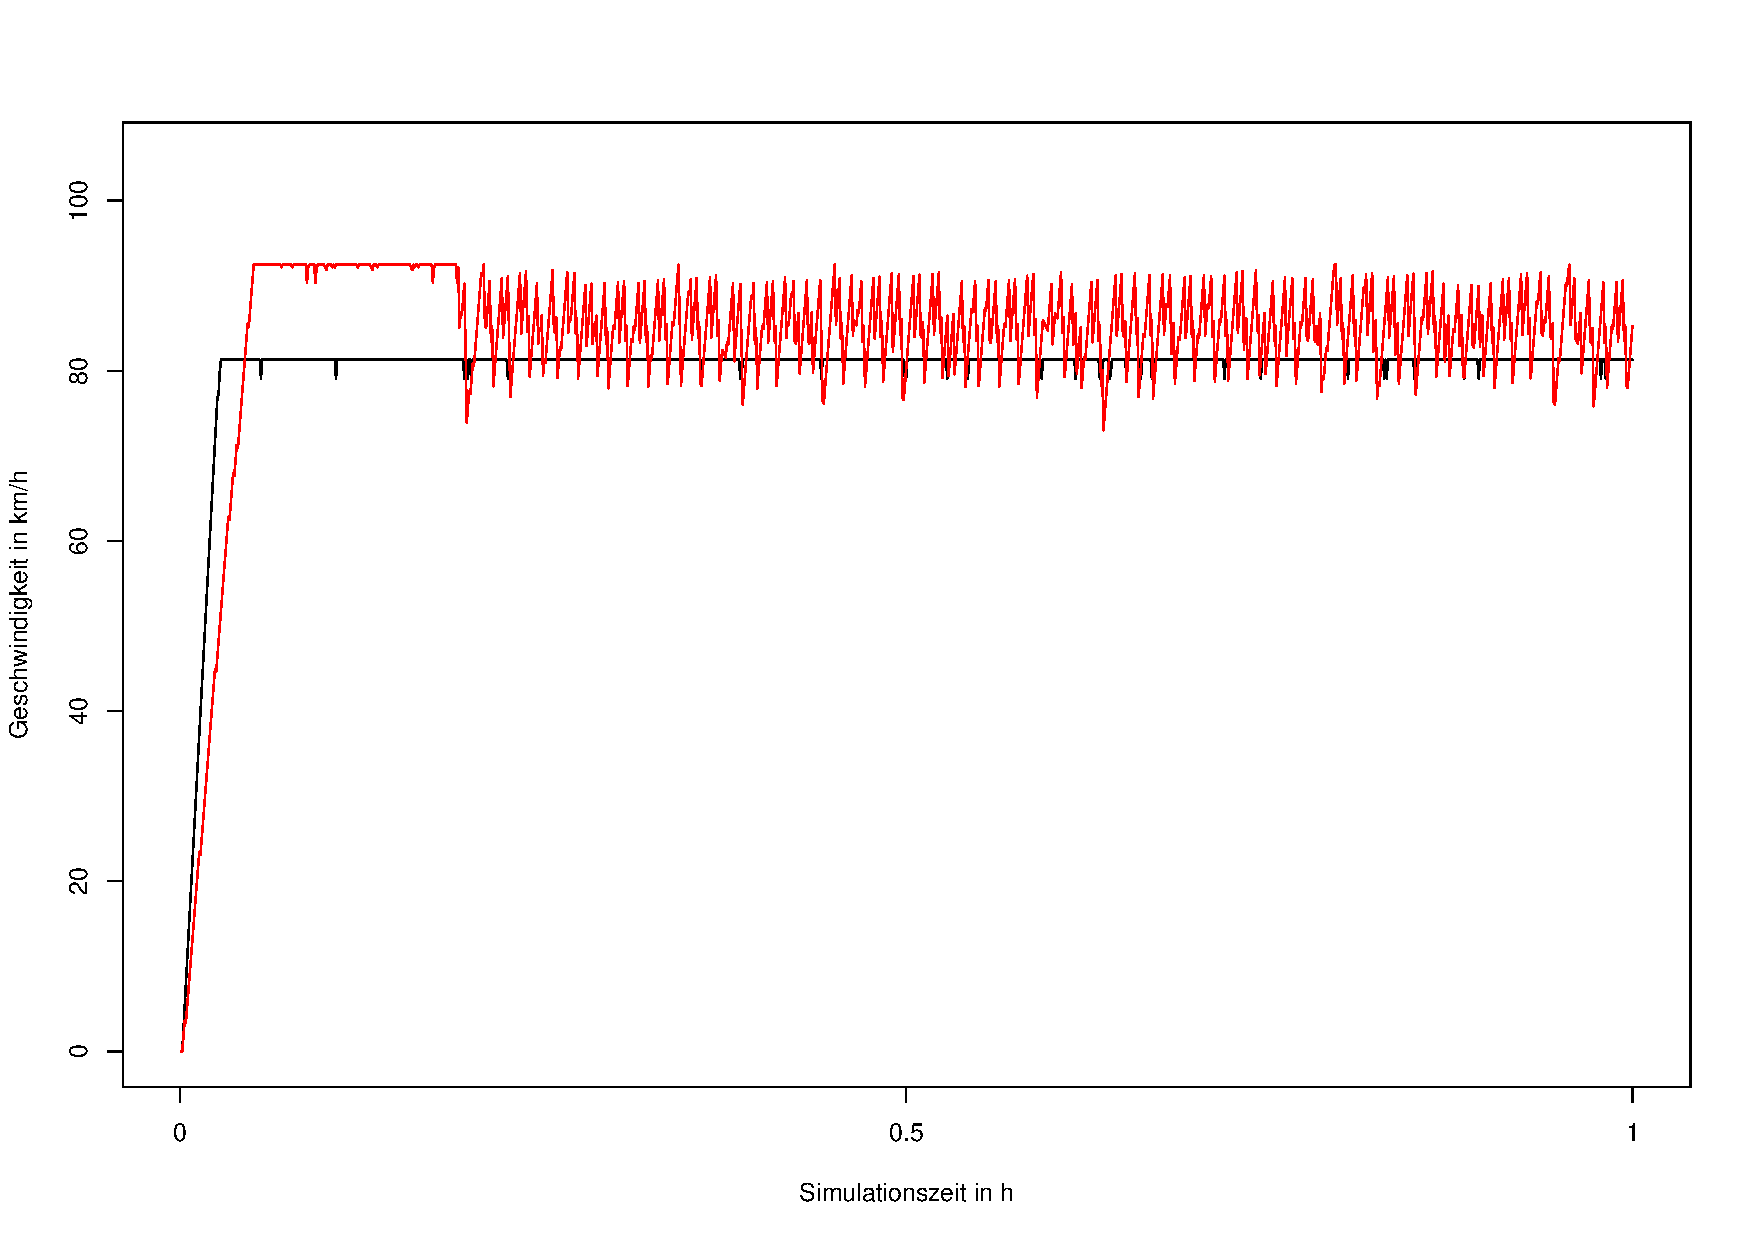
\includegraphics[width=0.45\textwidth]{test-speedcurve}\label{figure:test-speedcurve}}\qquad
   \subfigure[Plot der Zellpostionen]{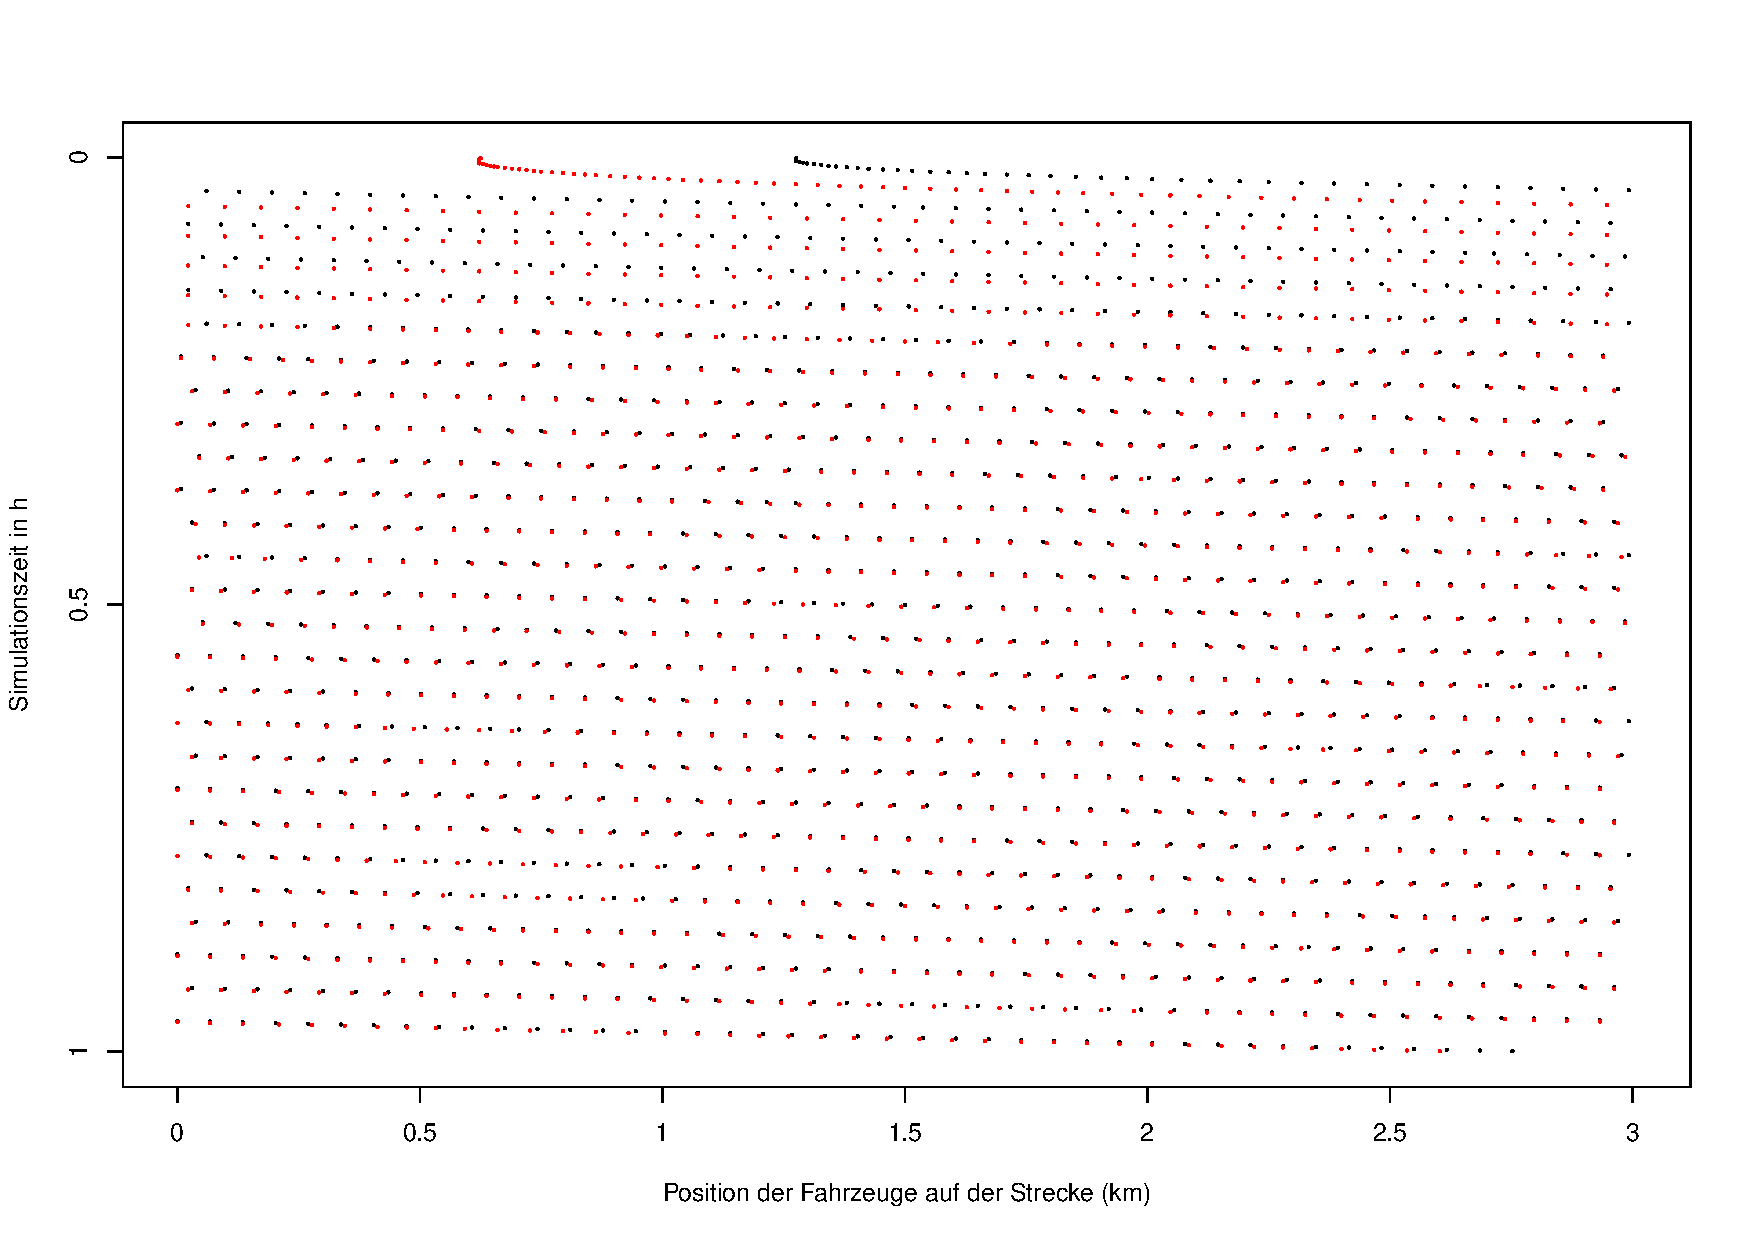
\includegraphics[width=0.45\textwidth]{test-cellcurve}\label{figure:test-cellcurve}} 
  \caption{Beispielkurven eines Testdurchlaufes}{\footnotesize Dauer: 1 h, Länge: 3 km, Zellgröße: 7,5 m, Zeitschritt: 0,05 min} 
  \label{figure:test-cell-speedcurves}
\end{figure}






\subsection{Verfeinerung des Agentenverhaltens}
\label{sec:verfeinerung-agentenplan}

Das Szenario für die Simulation kann über eine YAML-Datei individuell festgelegt werden.
Es gibt u.a. die Möglichkeit, die Streckenlänge, die Simulationsdauer, die Zellgröße und die Zeitschrittgröße anzugeben. 
Über Intervalle können die Geschwindigkeit und die Beschleunigungs- und Verzögerungswerte der Fahrzeuge eingestellt werden.



\subsubsection{Einstellmöglichkeiten in der Szenariokonfiguration}
\label{einstellungen-szenario}

%\subsubsection{Einstellmöglichkeiten für Zellgröße und Länge der Zeitschritte}

\paragraph*{Zellgröße:}
\label{zellgroesse-zeitschritte}
Die Entwicklung der Agentenpläne wurde ausschließlich in einer Simulationsumgebung mit einer Zellgröße von 7,5 m durchgeführt.
Als das Verhalten der Agenten zufriedenstellend war, wurde u.a. auch wegen der in \cref{sec:bremsverhalten} beschriebenen Bremsprobleme, getestet, inwiefern sich die Zelllänge verkürzen lässt und welchen Einfluss dies auf die Simulation hat.

% --- für Ausblick, Phil FB 27feb
% --- war vorerst nur solala formuliert
%Bei der Aufgrund der Parallelausführung der Simula-
%tion ergeben sich für die Entscheidungsgrundlagen der einzelnen Agenten unterschiedliche Vor-
%aussetzungen. Ein Fahrzeug sah z.B. regelmäßig die Position eines anderen Fahrzeugs aus dem
%vorangegangenen Zeitschritt und musste aufgrund dieser Informationen handeln. Hier konnten
%z.B. kritische Situationen nicht erkannt werden.

\paragraph*{Zeitschrittlänge:}
Die Länge der Zeitschritte lässt sich in der Konfiguration in Minuten oder Bruchteilen davon angeben. 
Dies stellte sich als unpraktikabel heraus, da z.B. eine Dauer von einer Sekunde durch den Dezimalbruch für $\frac{1}{60}$ angegeben werden müsste. Dieser weist aber eine Periodizität auf.

Begonnen wurde mit einer Zeitschrittlänge von 0,1 min, was sechs Sekunden entspricht. 
Diese Länge erwies sich als nicht sinnvoll, da zwischen den einzelnen Entscheidungszeitpunkten eine zu lange Zeitspanne liegt.

Die Entwicklung der Agentenpläne wurde mit einer Schrittlänge von drei Sekunden, 0,05 min, durchgeführt. Diese Länge genügte für diesen Zweck völlig.
Für die Tests auf Leistungsfähigkeit wurde die Schrittlänge dann auf 0.025 min, 1,5 Sekunden, reduziert.
\\
Ausführlich siehe \cref{sec:cellsize-timesteplength}.


%\subsubsection{Festlegen der Beschleunigungs-/Verzögerungswerte und der Sichtweite}

\paragraph*{Beschleunigung/Verzögerung:}
\label{beschl-verz}
Das originale Modell von Nagel und Schreckenberg legt Beschleunigung, Verzögerung und Sichtweite sehr einfach fest.
Bedingt durch die Zellgröße von \mbox{7,5 m}, die Ganzzahligkeit der Geschwindigkeit und die Zeitschrittlänge von 1 Sekunde ergeben sich Beschleunigungswerte von 7,5 $\frac{m}{s^{2}}$. 
Durch die Möglichkeit, die Geschwindigkeit innerhalb eines einzigen Zeitschrittes von der Maximalgeschwindigkeit \enquote{5} auf Null zu verringern, ergibt sich theoretisch eine Verzögerung von \mbox{37,5 $\frac{m}{s^{2}}$}.
Dies ist unrealistisch.

Die Simulationsumgebung arbeitet hier mit frei wähl- und einstellbaren Werten. 
In \cite{unfallrekonstruktion} sind die Werte für eine Vielzahl von Fahrzeugen aufgelistet. 
Für die Simulation wurden als real mögliche Werte Intervalle zwischen 3,5 und \mbox{7 $\frac{m}{s^{2}}$} für die Beschleunigung und zwischen 8 und \mbox{10 $\frac{m}{s^{2}}$} für die Verzögerung gewählt.
Der Wert wird für jedes Fahrzeug bei der Initialisierung im Rahmen dieser Intervalle zufällig festgelegt.
Die Dosierung der möglichen Beschleunigung bzw. Verzögerung wird im Agentenscript festgelegt.

\paragraph*{Sichtweite:}
\label{sec:sichtweite}
Für die Sichtweite ergibt sich im NaSch-Modell der theoretische Wert von \mbox{$ 5 \times $ 7,5 m}, also 37,5 Meter (bzw. je nach max. möglicher Geschwindigkeit  $ v_{max} $: \mbox{$ v_{max} \times $ 7,5 m}).
\\
Für die in der Agentensimulation vorliegenden \enquote{realen} Bremsvorgänge ist diese Entfernung unzureichend. 

Die Sichtweite im Straßenverkehr kann laut \cite{sichtweite} aufgrund von physiologischen und psychologischen Gründen in drei Zonen eingeteilt werden:
\begin{itemize}
\itemsep0em
	\item \enquote{Fernorientierung/Information}, auf Autobahnen etwa zwischen 600 und 360 Metern
	\item \enquote{Bereitschaft/Entscheidung}, etwa zwischen 360 und 110 Metern
	\item \enquote{Nahorientierung/Handlung}, unter 110 Metern
\end{itemize}

Die für Reaktionsträgheit maßgebliche Komponente Mensch fehlt im Agentensystem. 
Darum muss die Zone der Fernorientierung nicht ausgeschöpft werden.
Ein Wert der Sichtweite mittig im Intervall der Entscheidungszone genügt, um bis zum Beginn der Handlungszone \enquote{tätig zu werden}.

Für die Sichtweite wurde der Wert 250 m gewählt.
Dieser trifft die o.g. Vorgabe und liegt ungefähr mittig im Intervall der Entscheidungszone. Den Agenten sollte diese Strecke genügend Raum für Reaktionen geben. 
In den Agentenplänen wird schließlich die Handlung durch Bedingungen auf einen Bereich unter 110 m beschränkt.


\subsubsection{Einstellmöglichkeiten im Agentenverhalten (Parameter)}

\paragraph*{Festlegen der Trödelparameter:}
\label{sec:lingersweetspot}

Im Originalmodell wird dem jeweiligen Fahrzeug im Trö"-del"-fall eine Geschwindigkeitseinheit wieder abgezogen. 
In jenem Zeitschritt erfolgt somit keine Beschleunigung, bzw. bei Fahren mit max. möglicher Geschwindigkeit wird diese reduziert. 
Auf das Abbremsen vor einem Hindernis hat dies keinen Einfluss, weil die mögliche Geschwindigkeit an Größe der vorhandenen Lücke angepasst werden kann.

Für die Simulation musste ein Wert gefunden werden, der dieses Verhalten näherungsweise nachbildet.
Im Laufe mehrerer Testdurchgänge schien eine Intensität der Verzögerung von \texttt{0,3} die getätigte Beschleunigung am besten zu egalisieren. 
Hierbei ist noch die Streuung der Be"-schleu"-ni"-gungs- und Verzögerungswerte zu beachten, sodass das Trödeln unterschiedlich große Effekte haben kann.

Für das Abbremsen in der Agentensimulation kann sich das Trödeln positiv auf den Bremsweg auswirken, da ein zusätzlicher Bremsimpuls erzeugt wird. 
Hier wird im allgemeinen aber in Summe eine Verzögerung über dem max. real möglichen Wert erziehlt.
\\
Aufgrund der \enquote{Bremsprobleme}, siehe \cref{sec:bremsverhalten}, wurde dies aber vorerst in Kauf genommen.

Für die Trödelwahrscheinlichkeit $ p_{linger} $ wurde beobachtet, dass deren Höhe bei Werten \mbox{$\leq$ \texttt{0,5}} nur einen kleinen Einfluss auf die max. mögliche Geschwindigkeit hatte.
In den Testdurchläufen konnte diese Geschwindigkeit erreicht werden.
\\
Bei einer größeren Wahrscheinlichkeit wurde die mögliche Geschwindigkeit innerhalb der 30 Minuten Simulationszeit teilweise nicht oder nur schwer erreicht.
Bei einem Wert von \texttt{0,7} ergab sich ein Durchlauf, bei dem die 20 km/h nicht erreicht wurden, siehe \cref{figure:linger-0ko7-2nd}.

\begin{figure}[hptb]
  \centering 
   \subfigure[1. Durchlauf]{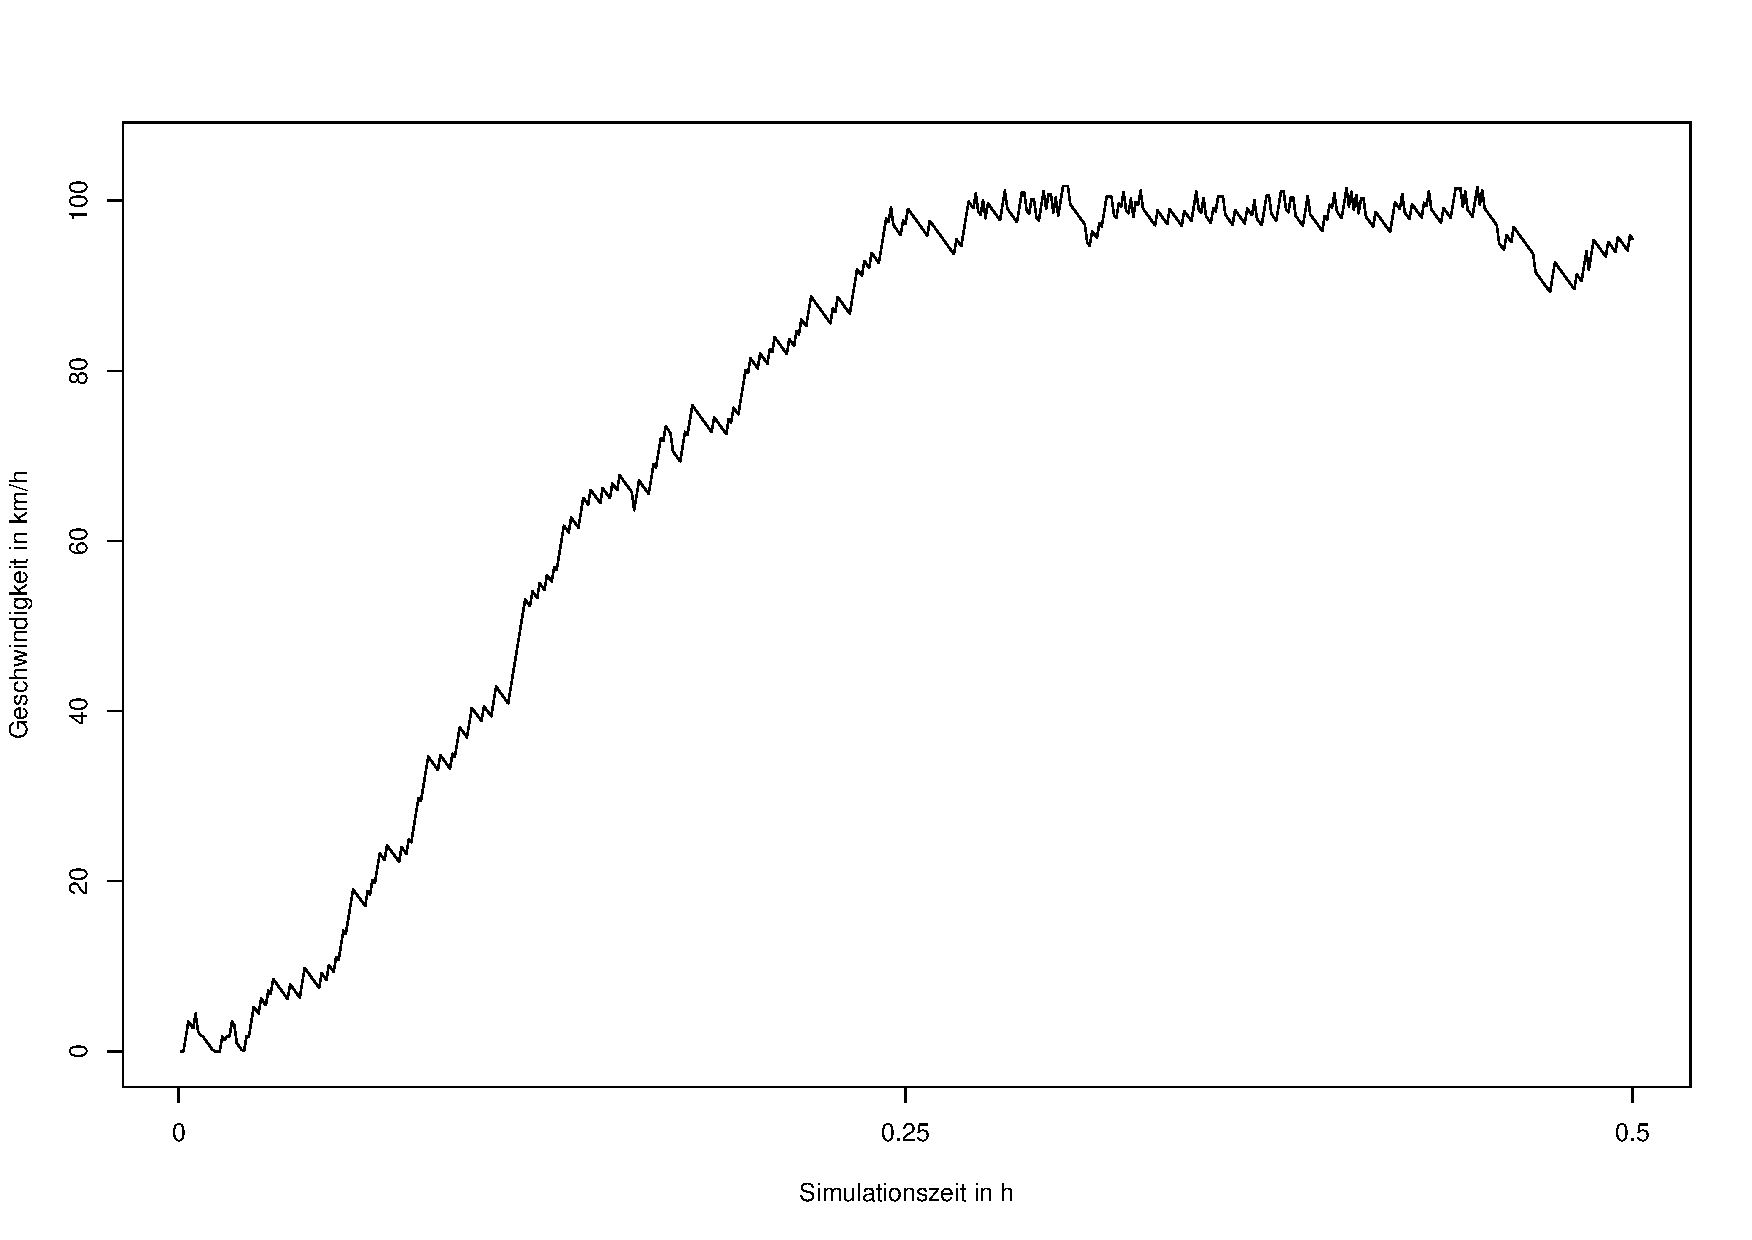
\includegraphics[width=0.3\textwidth]{linger-0ko7}\label{figure:linger-0ko7-1st}}\qquad
   \subfigure[2. Durchlauf]{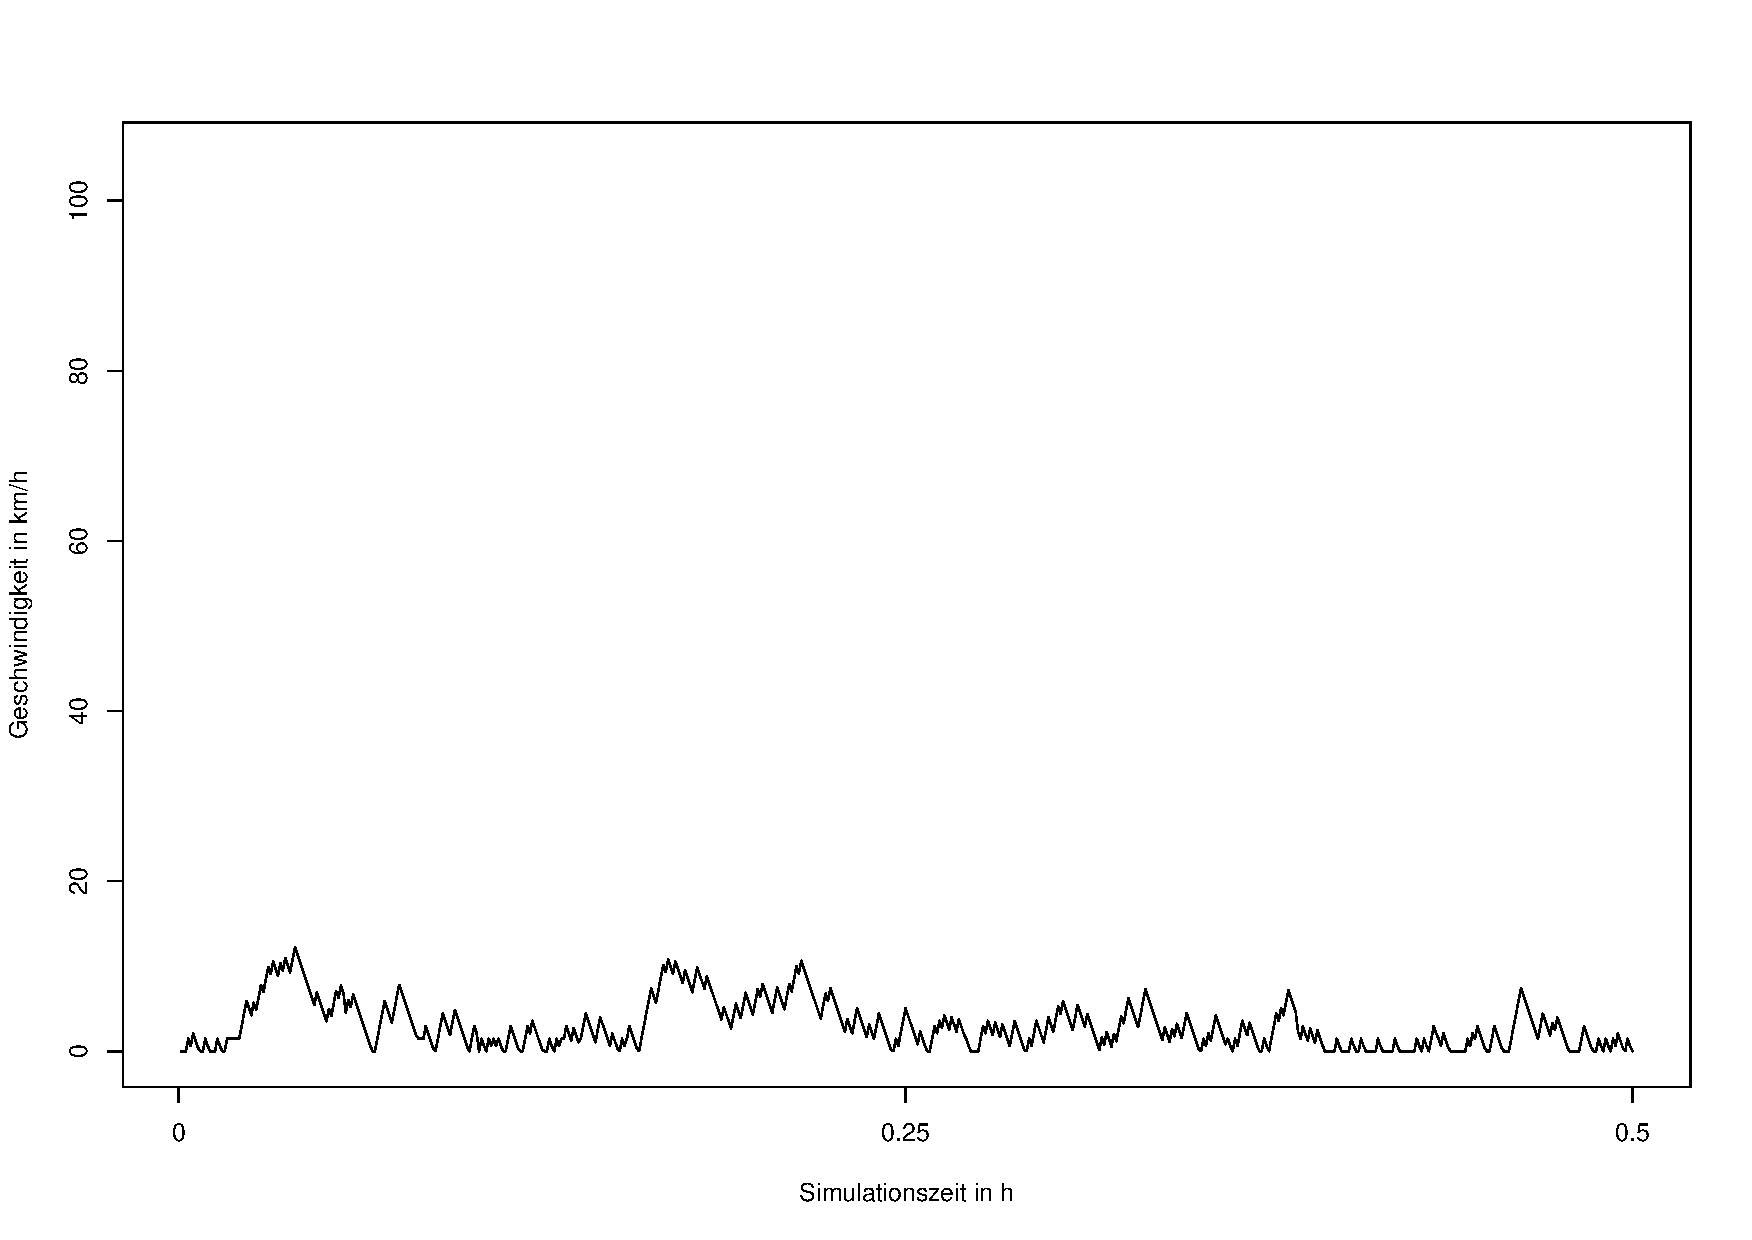
\includegraphics[width=0.3\textwidth]{linger-0ko7-2nd}\label{figure:linger-0ko7-2nd}}\qquad
   \subfigure[3. Durchlauf]{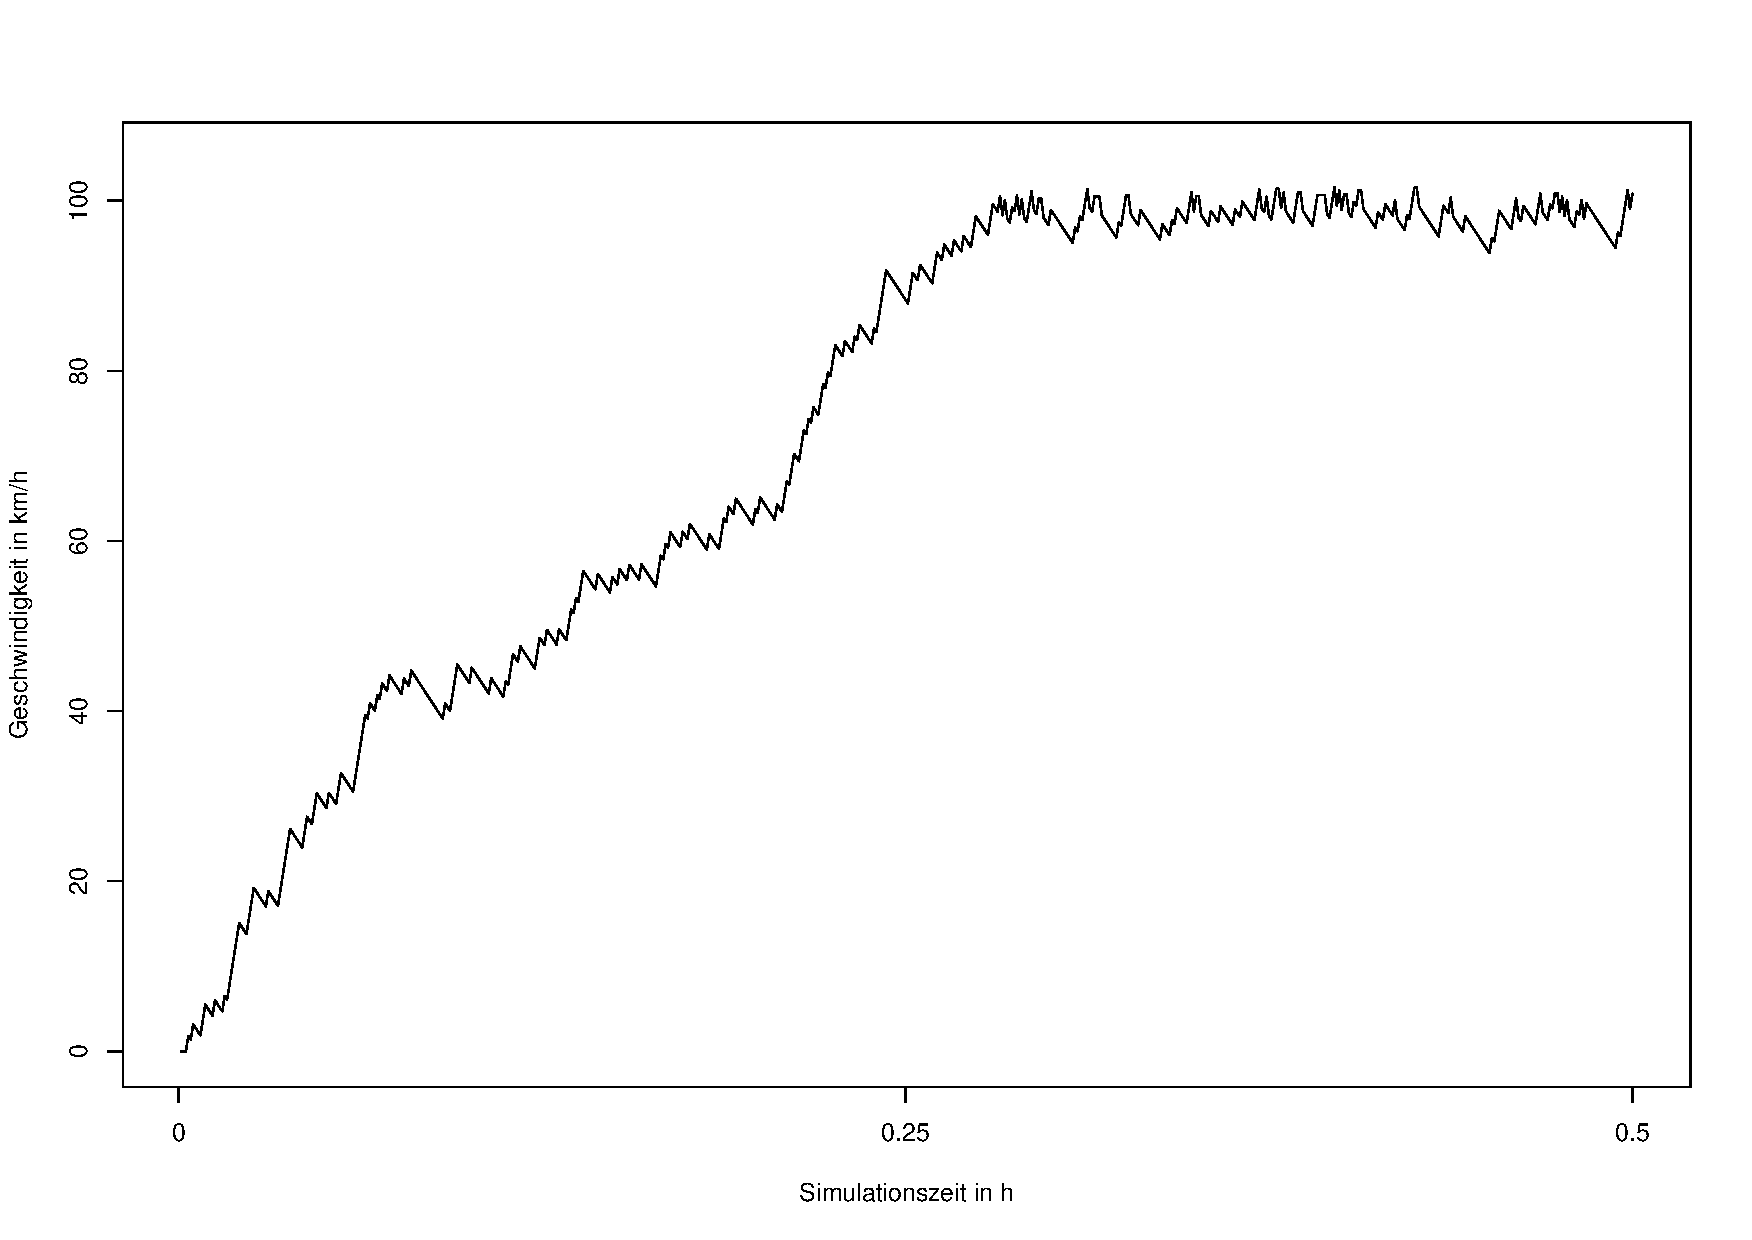
\includegraphics[width=0.3\textwidth]{linger-0ko7-3rd}\label{figure:linger-0ko7-3rd}} 
  \caption{Geschwindigkeitskurven bei $p_{linger}$ = 0,7}
  \label{figure:linger-0ko7}
\end{figure}

Eine merkliche Veränderung trat auch bei der Beschleunigung der Fahrzeuge auf.
Je höher der Wert für $ p_{linger} $, desto flacher wurde im allgemeinen der Anstieg bei der Beschleunigung, siehe \cref{figure:linger-0ko1-3-5}.
Außerdem bilden sich mit zunehmender Trödelwahrscheinlichkeit deutlichere Geschwindigkeitseinbrüche aus - z.B. \cref{figure:linger-0ko1} vs. \cref{figure:linger-0ko3}.

\begin{figure}[hptb]
  \centering 
   \subfigure[Durchlauf $p_{linger}$ = 0,1]{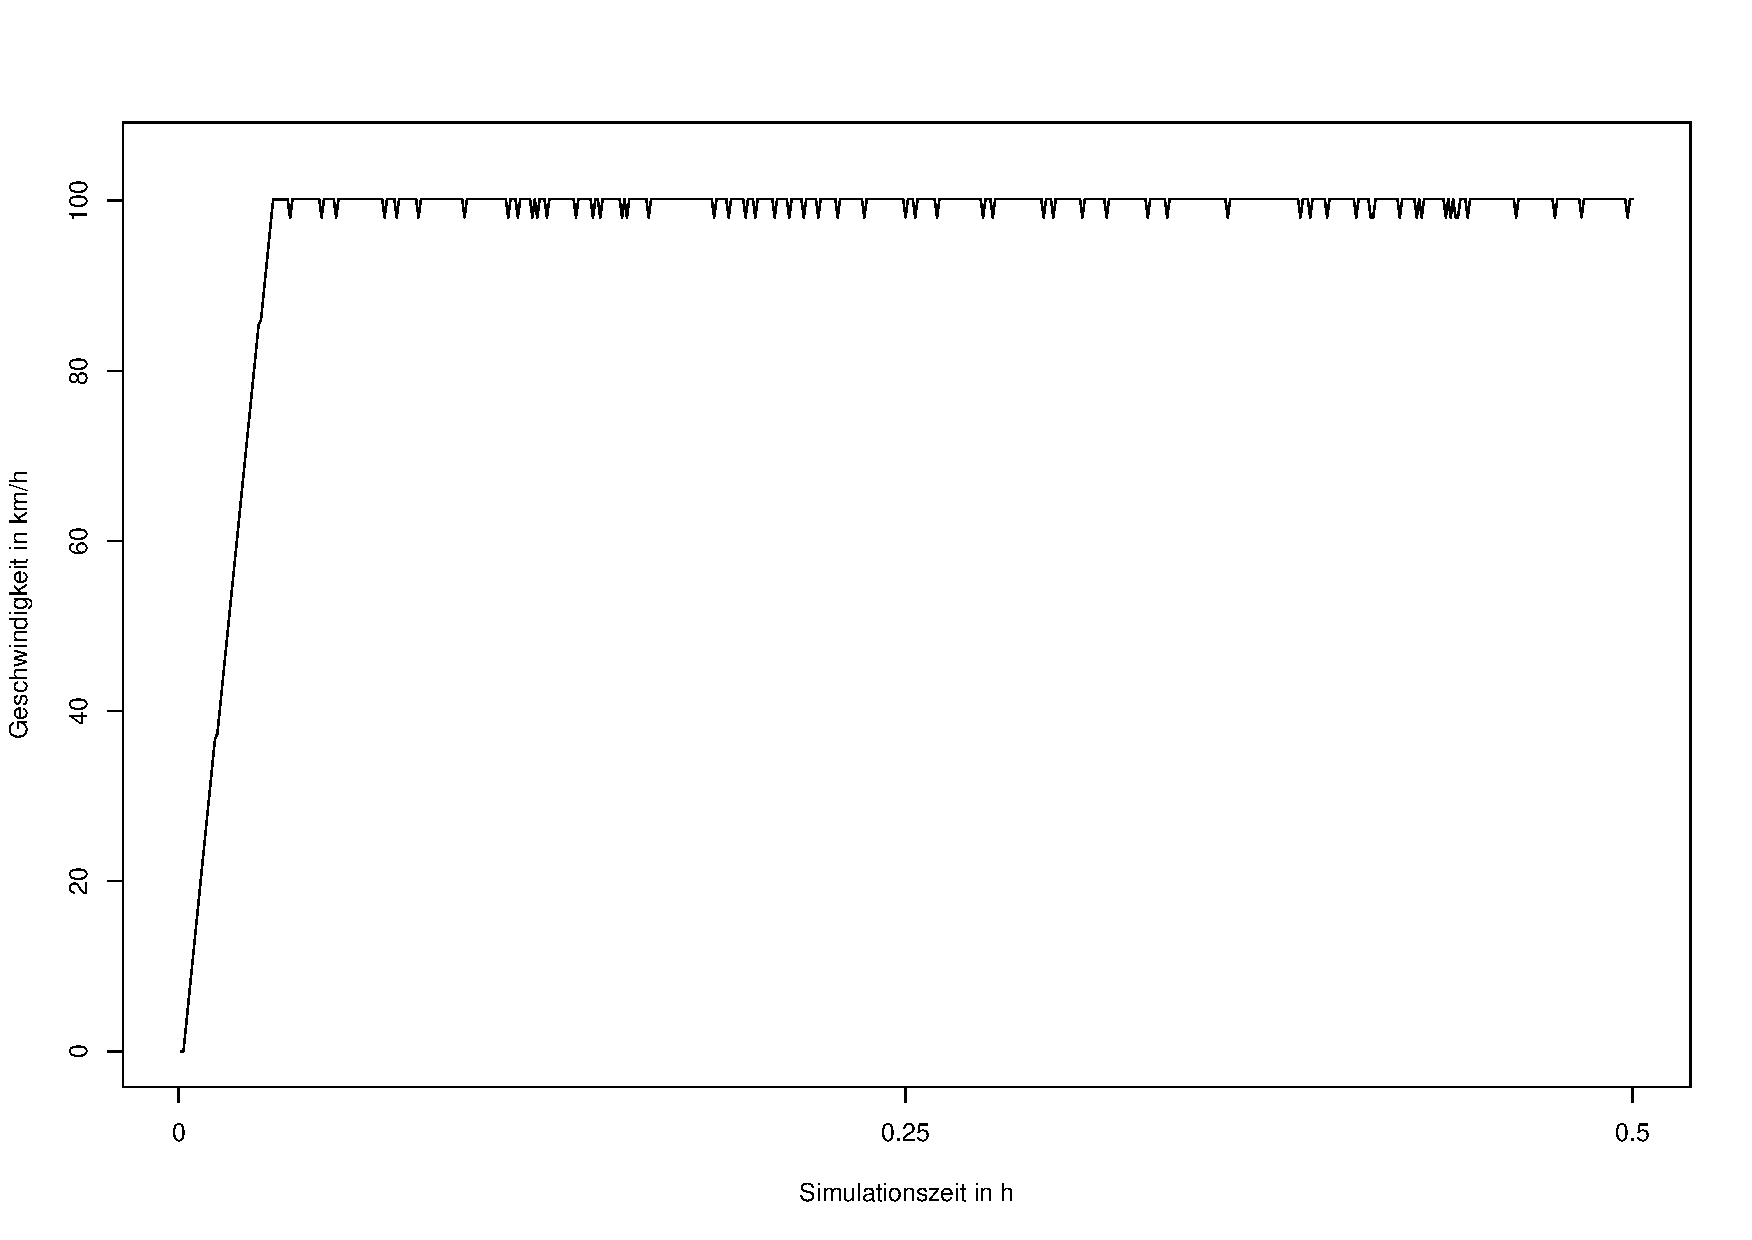
\includegraphics[width=0.3\textwidth]{linger-0ko1-3rd}\label{figure:linger-0ko1}}\qquad
   \subfigure[Durchlauf $p_{linger}$ = 0,3]{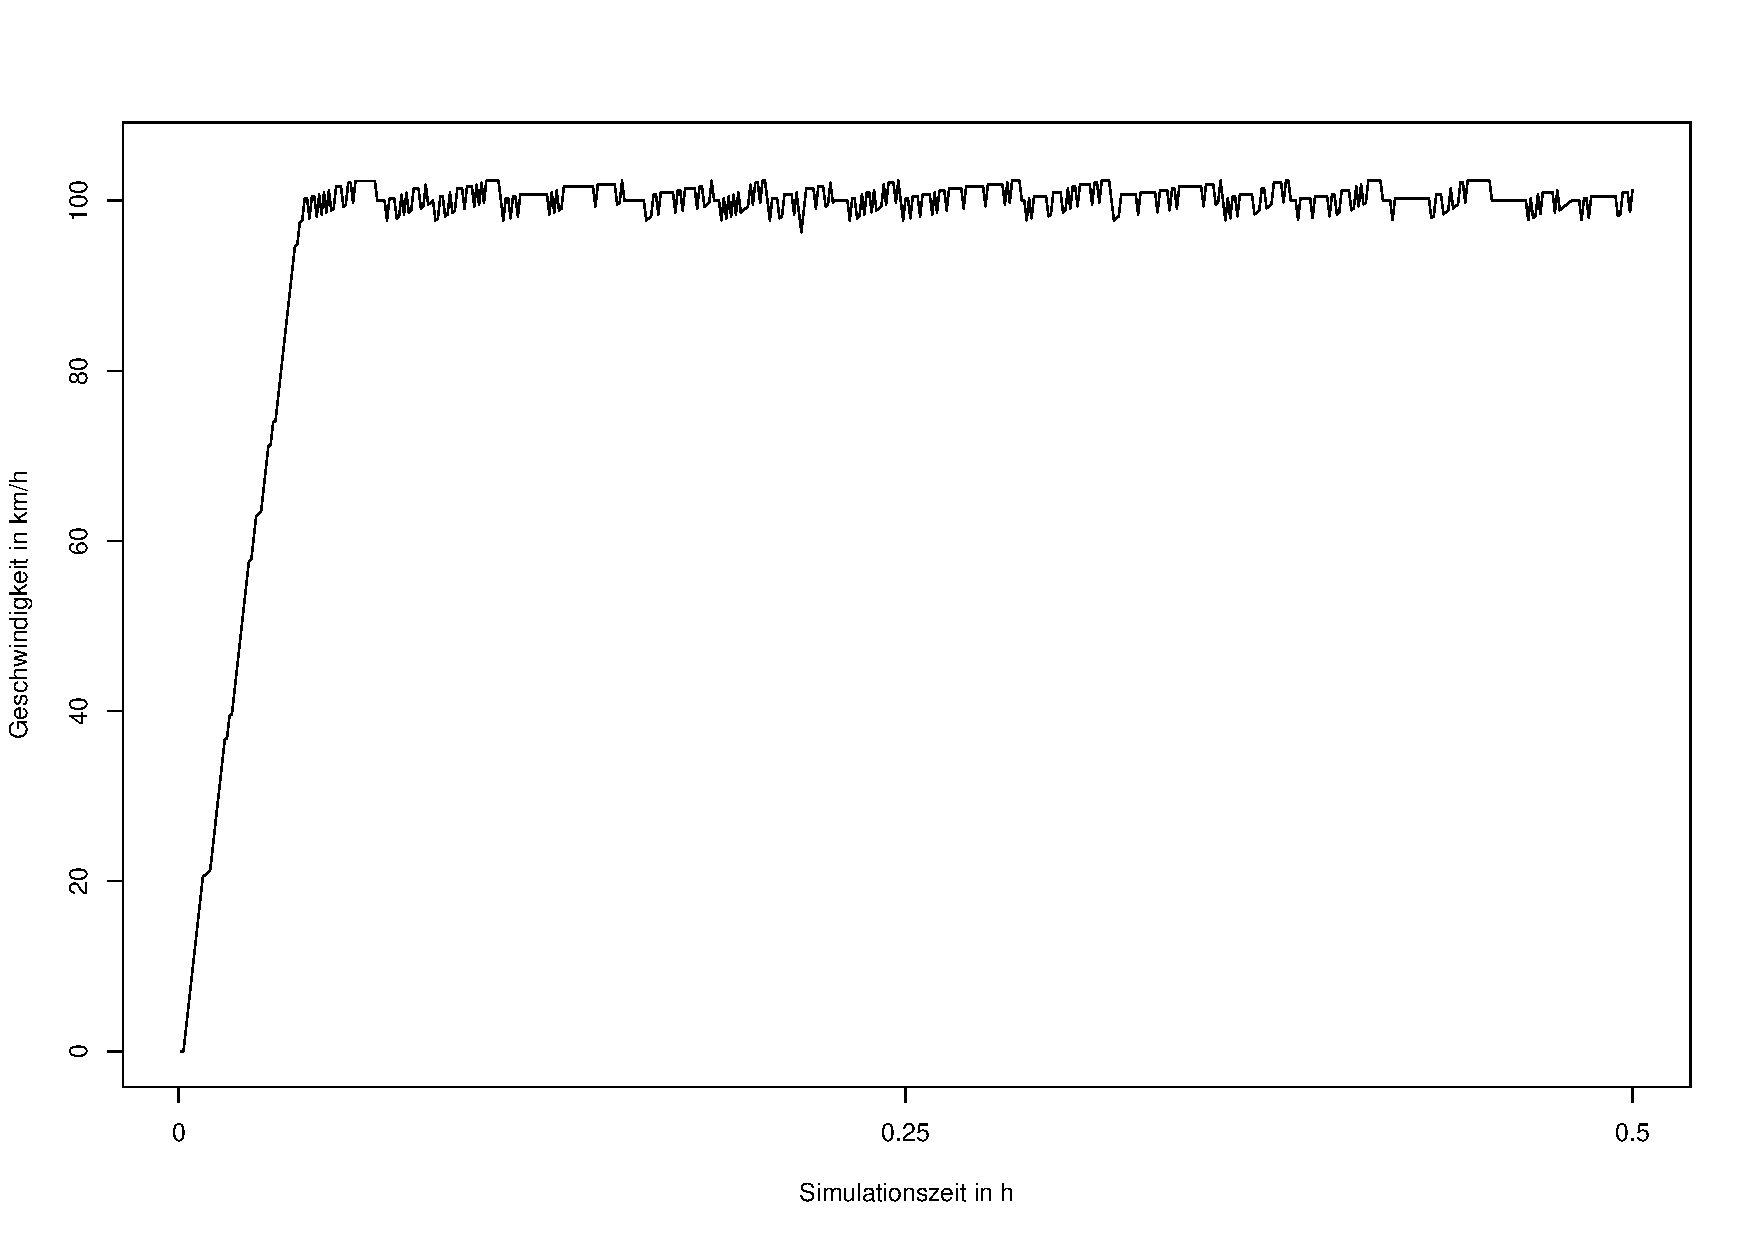
\includegraphics[width=0.3\textwidth]{linger-0ko3}\label{figure:linger-0ko3}}\qquad
   \subfigure[Durchlauf $p_{linger}$ = 0,5]{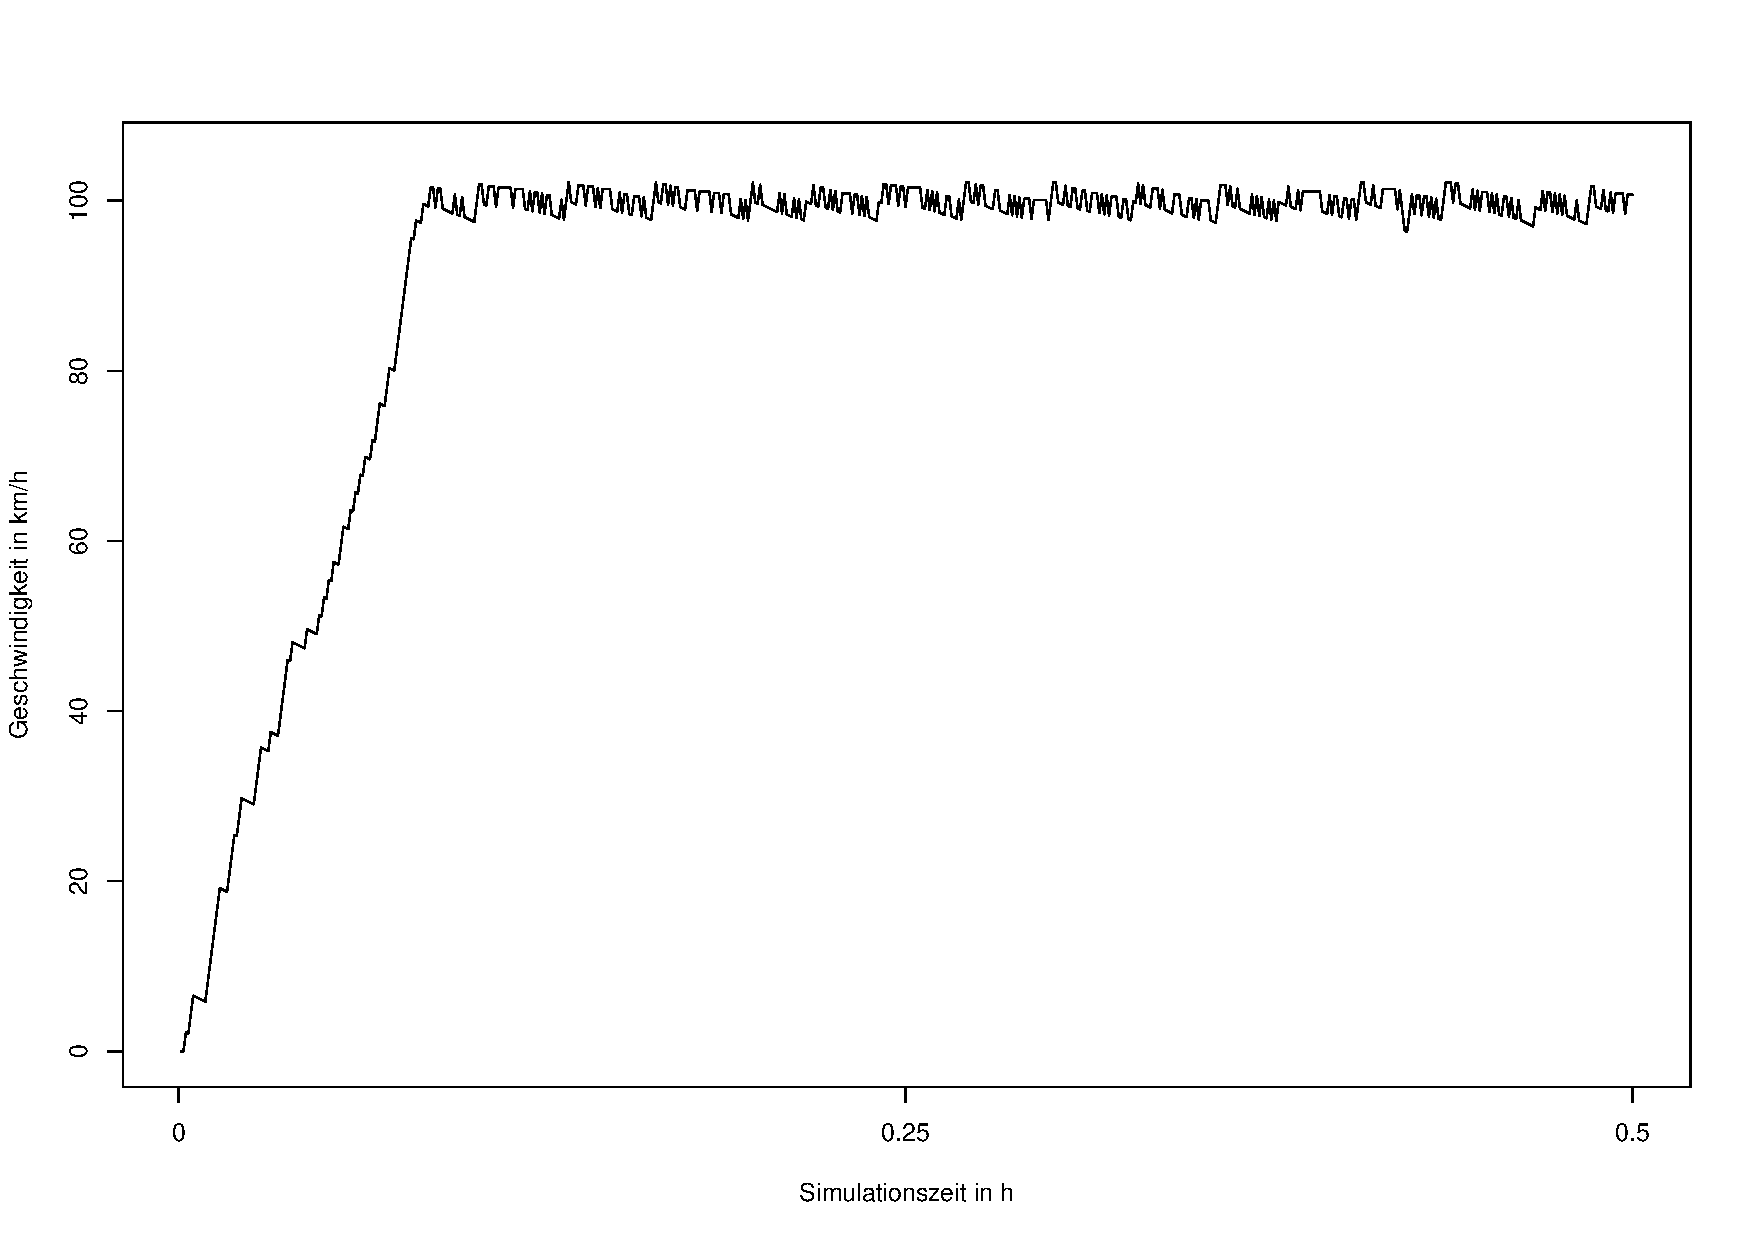
\includegraphics[width=0.3\textwidth]{linger-0ko5-3rd}\label{figure:linger-0ko5}} 
  \caption{Beispiele für Geschwindigkeitskurven bei unterschiedlichen Werten für $p_{linger}$}
  \label{figure:linger-0ko1-3-5}
\end{figure}

Weiterhin hat die Trödelwahrscheinlichkeit bei gleicher Höhe, scheinbar abhängig von den gefahrenen Geschwindigkeiten, unterschiedliche Einflüsse auf den Verkehrsfluss.
\\
Bei einer max. möglichen Geschwindigkeit von 50 km/h erzeugt erst eine Wahrscheinlichkeit von \texttt{0,5} einen merklichen Effekt. Für eine Geschwindigkeit von 100 km/h ist dies bei gleicher Fahrzeuganzahl bereits bei einem Wert von \texttt{0,3} der Fall.
\\
Bei Werten darüber hinaus wurde beobachtet, dass die Beschleunigung eines oder mehrerer Fahrzeuge so gehemmt wurde, dass ein Erreichen der möglichen Geschwindigkeiten für alle im System befindlichen Fahrzeuge nicht möglich war.

Für die Dauertests mit einer max. möglichen Geschwindigkeit von 100 km/h wurden die Parameter im \texttt{linger}-Plan somit auf Wahrscheinlichkeit von \texttt{0,3} und eine Bremsintensität von \texttt{0,3} festgelegt.





\subsection{Anpassungen der Simulationssoftware}
\label{sec:anpassungen-probleme}

Einer der Hauptunterschiede zur Softwareversion des Workshops ist, dass die Simulationen hier auf einer unendlichen Strecke stattfinden, wie bereits in \cref{sec:na-sch} für die Versuche von Nagel und Schreckenberg beschrieben.

Diese Unendlichkeit existiert dabei allerdings nur virtuell.
Fahrzeuge, die das Ende der Strecke passieren, werden mit gleichen Verhaltenswerten am Anfang wieder eingesetzt.
Der Abstand vom Anfang der Strecke richtet sich dabei nach der letzten Position am Streckenende und der aktuellen Geschwindigkeit.

Das Umsetzen selbst bereitete keine Probleme, allerdings resultierten solche aus dieser Unterbrechung der Strecke.



\subsubsection{Schwierigkeiten bei der Simulation der Ringform der Strecke}
\label{sec:probleme-ringform}

Die Streckenunterbrechung führte dazu, dass es eine Pause in der Sichtbarkeit der Fahrzeuge untereinander gab, wenn sich diese an unterschiedlichen Enden der Strecke befanden.
Aufgrund dieser \enquote{Unsichtbarkeit} war es unmöglich, eine Abstandsberechnung zwischen den einzelnen Fahrzeugen durchzuführen und führte zu einer freien Beschleunigung, da eine freie Strecke vermutet wurde.

Nachfolgend ist dies anhand des Log-Auszuges einer Simulation mit zwei Fahrzeugen, \texttt{vehicle0} und \texttt{vehicle20}, dargestellt. 
(\enquote{...} bezeichnet Kürzungen der Ausgabe.)

In Zeitschritt 315 war Fahrzeug \texttt{vehicle20} gerade noch in der letzten Zelle der Fahrbahn und überschreitet diese Grenze einen Zeitschritt später.
Die Beliefliste beider Fahrzeuge ist ab dem Schritt 316 leer.
Erst vier Zeitschritte später befindet sich auch das Folgefahrzeug (\texttt{vehicle0}) am Anfang der Fahrspur und ist ab Zeitschritt 320 wieder für Fahrzeug \texttt{20} sichtbar (andersherum ebenso).

\footnotesize\begin{verbatim}
----- step 315 ----------------
      vehicle0   -> BELIEFLIST   [view/vehicle[id[vehicle20], ... direction[forward[]]]]]]
      vehicle20   -> BELIEFLIST   [view/vehicle[id[vehicle0], ... direction[backward[]]]]]]
      vehicle0   in lane   1   in cell   331.0   @   87.11188616490347   kph
      vehicle20   in lane   1   in cell   400.0   @   88.65039571533352   kph
----- step 316 ----------------
      vehicle0   -> BELIEFLIST   []
      vehicle20   -> BELIEFLIST   []
      vehicle0   in lane   1   in cell   345.0   @   87.89778423377561   kph
      vehicle20   in lane   1   in cell   14.0   @   88.65039571533352   kph
----- step 317 ----------------
...
----- step 318 ----------------
...
----- step 319 ----------------
      vehicle0   -> BELIEFLIST   []
      vehicle20   -> BELIEFLIST   []
      vehicle0   in lane   1   in cell   387.0   @   89.01152857206483   kph
      vehicle20   in lane   1   in cell   56.0   @   88.65039571533352   kph
----- step 320 ----------------
      vehicle0   -> BELIEFLIST   [view/vehicle[id[vehicle20], ... direction[forward[]]]]]]
      vehicle20   -> BELIEFLIST   [view/vehicle[id[vehicle0], ... direction[backward[]]]]]]
      vehicle0   in lane   1   in cell   1.0   @   89.79742664093698   kph
      vehicle20   in lane 1 in cell 70.0 @ 88.65039571533352 kph
\end{verbatim}
\normalsize

Für die Simulation mit mehreren Fahrzeugen stellte dies insbesondere ein Problem dar, weil eine Stauwelle, die sich in ihrer Rückwärtsbewegung dem Anfang der Strecke näherte, von Fahrzeugen am Ende der Strecke nicht erkannt werden konnte.
Demzufolge gab es auch keine Reaktion auf das Hindernis.

Dies führte zu dem Verhalten, dass Fahrzeuge vom Ende der Strecke an den Anfang gesetzt werden sollten, dort aber nicht in eine freie Zelle gesetzt werden konnten.
Die Simulationsumgebung sieht hier vor, dass das Fahrzeug auf die freie Zelle (in Fahrtrichtung) hinter das jeweils letzte Fahrzeug gesetzt wird.
\\
Softwareseitig ist Zelle \texttt{0} die erste zu besetzende Zelle einer Lane. Die freie Zelle hinter dem Fahrzeug war hier aber Zelle \texttt{-1} und nicht die letzte Zelle am Lane-Ende.
Zudem wurde ein Fahrzeug, das sich bereits dort befand, jeweils noch ein Feld weiter nach hinten gesetzt und das neue Fahrzeug dazwischen einfügt.
Dies setzte sich kaskadierend in den negativen Bereich fort.
\\
Hierbei handelt es sich um einen separaten Fehler, der durch ersteren erkannt werden konnte.

Es ergab sich bei einigen Simulationsläufen ein Häufung von Positionspunkten im negativen Teil der Strecke.
In der Simulation in \cref{figure:negativ-sammeln} trat das Problem direkt am Anfang des Durchlaufs aufgrund der langen Standzeit (siehe auch \cref{sec:accelerategroove}) des direkt am Anfang der Lane verorteten Fahrzeuges auf und konnte über die Simulationsdauer nicht abgebaut werden.
\begin{figure}[hptb]
 \centering
 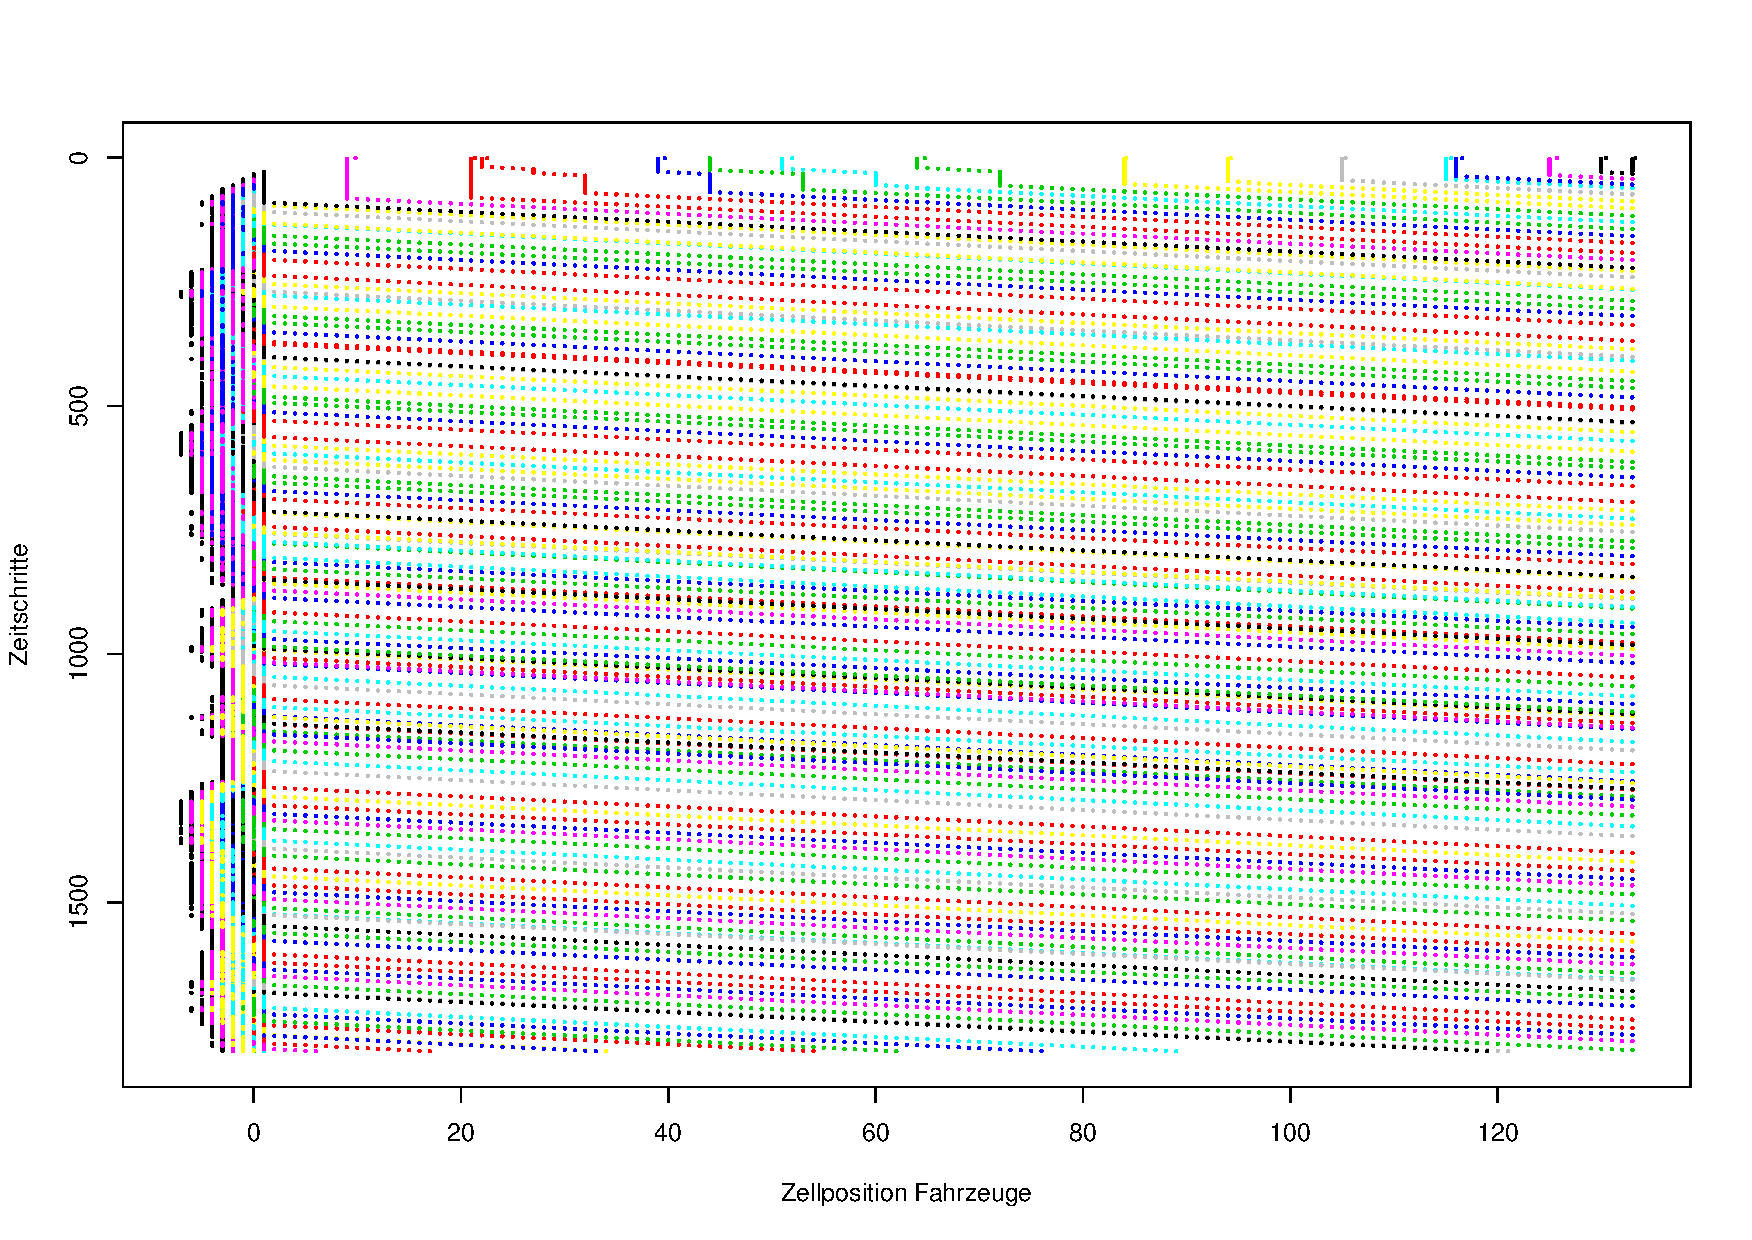
\includegraphics[width=0.9\textwidth]{negativ-sammeln}
 \caption[Punktehäufung im negativen Bereich]
 		 {Häufung der Punkte im negativen Bereich (Position-Zeit-Diagramm)}
 \label{figure:negativ-sammeln}
\end{figure} 

In \cref{figure:view-range-no-clip} wird die Problematik des \enquote{Nicht-Sehens} beispielhaft am Sichtfeld des gelben Fahrzeugs grafisch verdeutlicht. 
Gleiches gilt analog für die rückwärtige Sicht des violetten Fahrzeugs.

\begin{figure}[hptb]
  \centering
    \subfigure[ohne Umbruch]{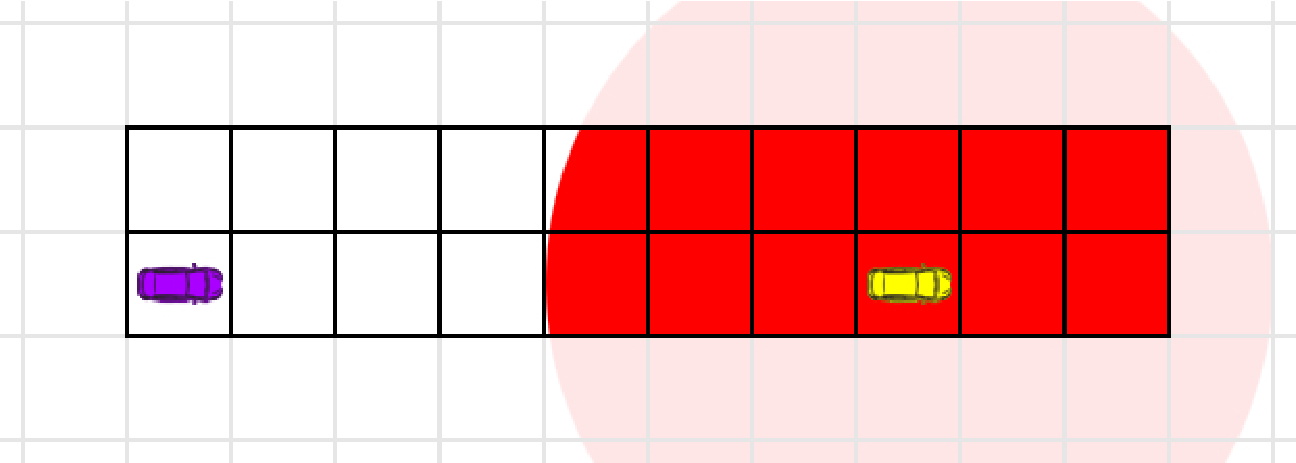
\includegraphics[width=0.8\textwidth]{view-range-no-clip}\label{figure:view-range-no-clip}} \\
    \subfigure[mit Umbruch]{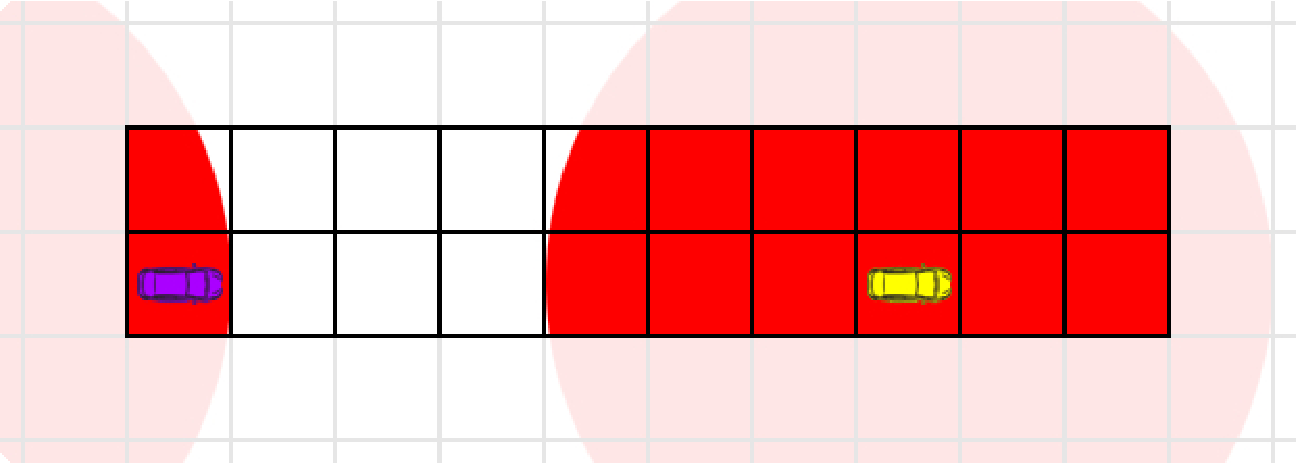
\includegraphics[width=0.8\textwidth]{view-range-clip}\label{figure:view-range-clip}}
  \caption[Umbrechen des Sichtfelds eines Fahrzeugs am Ende der Lane]
          {Sichtfeld des gelben Fahrzeugs am Ende der Lane}
          {\footnotesize Quelle Auto-Silhouette: vecteezy.com}
  \label{figure:view-range-no-clip-clip}
\end{figure}

Für die Erstellung der sichtbaren Umgebung der Fahrzeuge werden die Zellen zur \enquote{view range}, die sich innerhalb der im Szenario angegebenen Entfernung befinden.
Diese werden als relative Angaben mit dem jeweiligen Fahrzeug als Mittelpunkt gespeichert und in jedem Zeitschritt auf reale Koordinaten umgerechnet.
Befindet sich dann ein anderes Fahrzeug in einer dieser Zellen, befindet es sich im Sichtfeld und eine Entfernung und Richtung werden berechnet.

Die Schwierigkeit bestand darin, die Zellen am jeweils anderen Ende der Strecke mit in die Liste der relativen Zellpositionen aufzunehmen, siehe \cref{figure:view-range-clip}, und virtuelle Zellpositionen korrekt auf reale Positionen umzurechnen.

\begin{figure}[hptb]
  \centering
    \subfigure[vorher: Durchlauf mit Fehler]{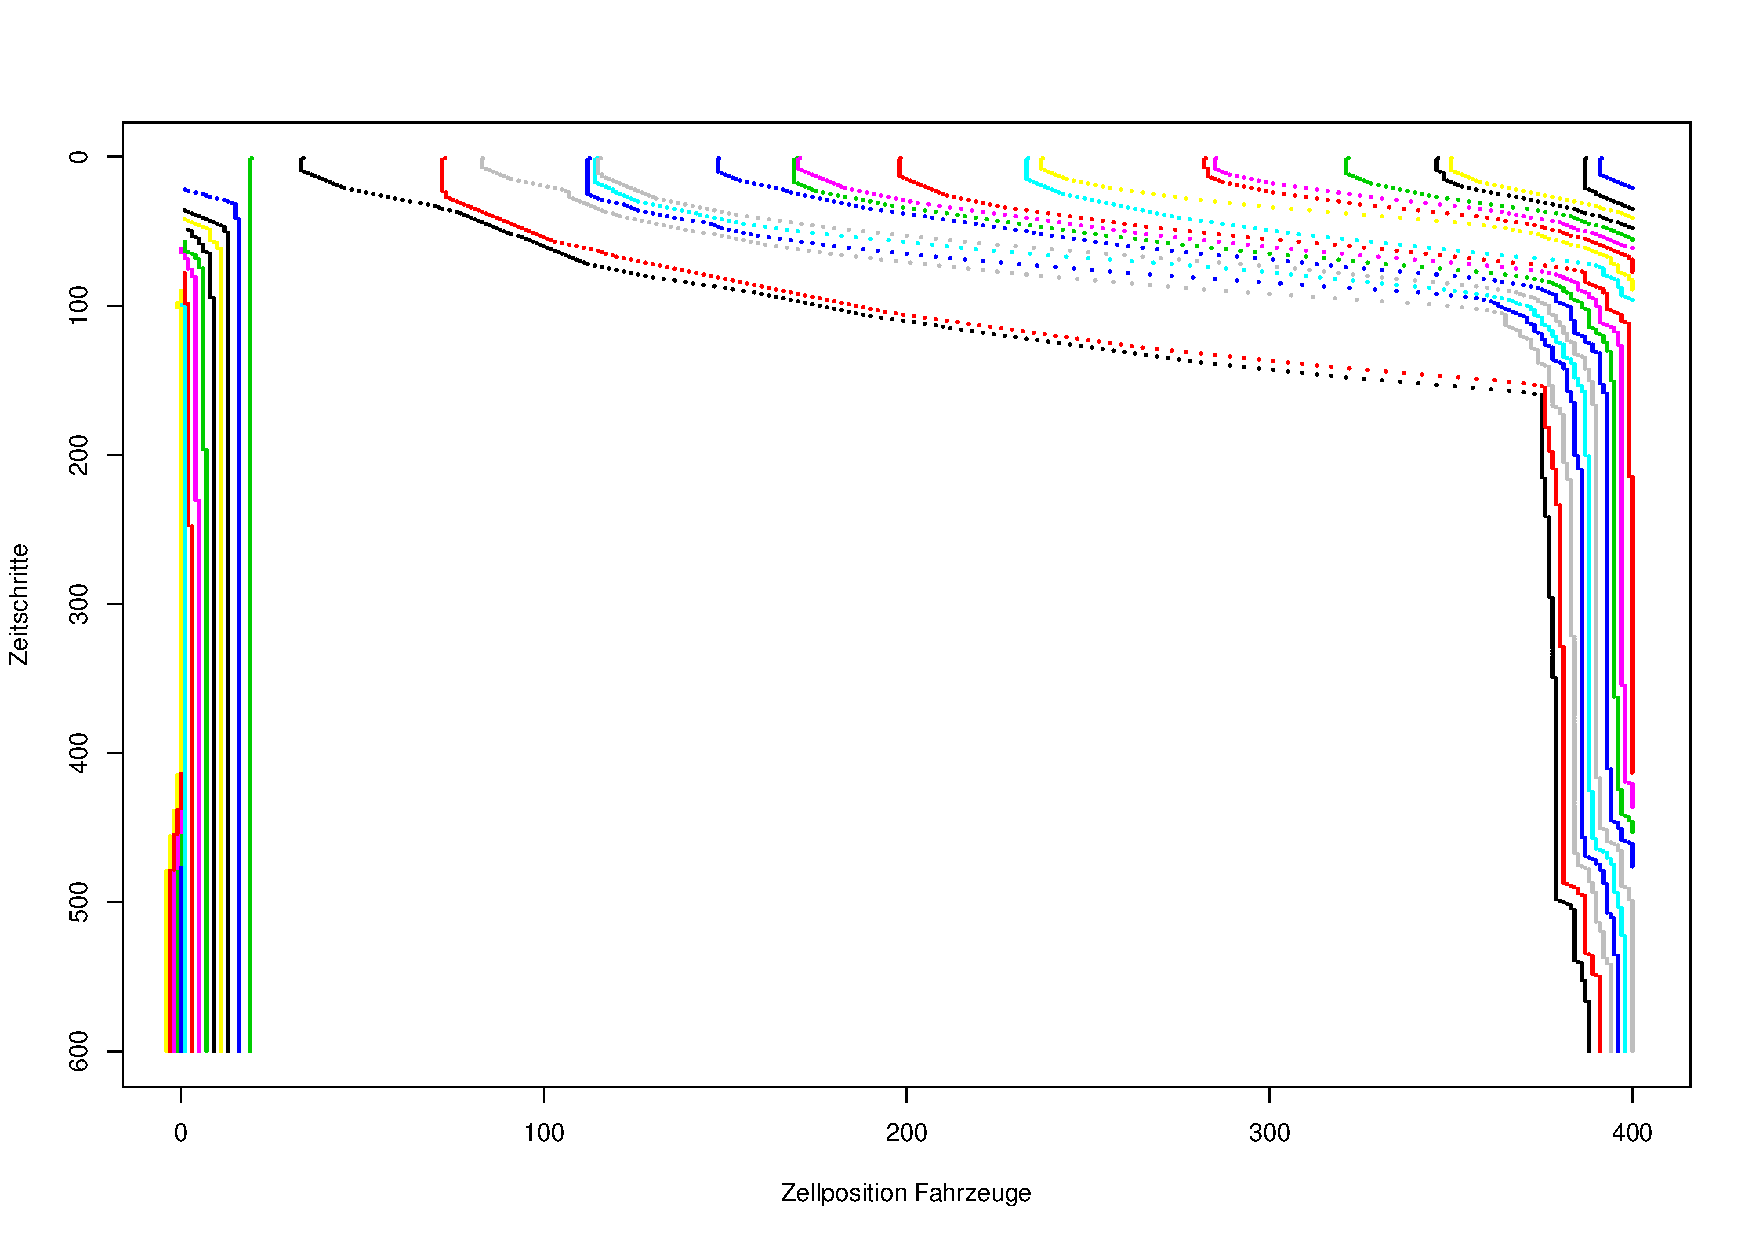
\includegraphics[width=0.45\textwidth]{go-negative_release-v175_fail}\label{figure:go-negative-fail}} \qquad 
    \subfigure[nachher: Durchlauf ohne Fehler]{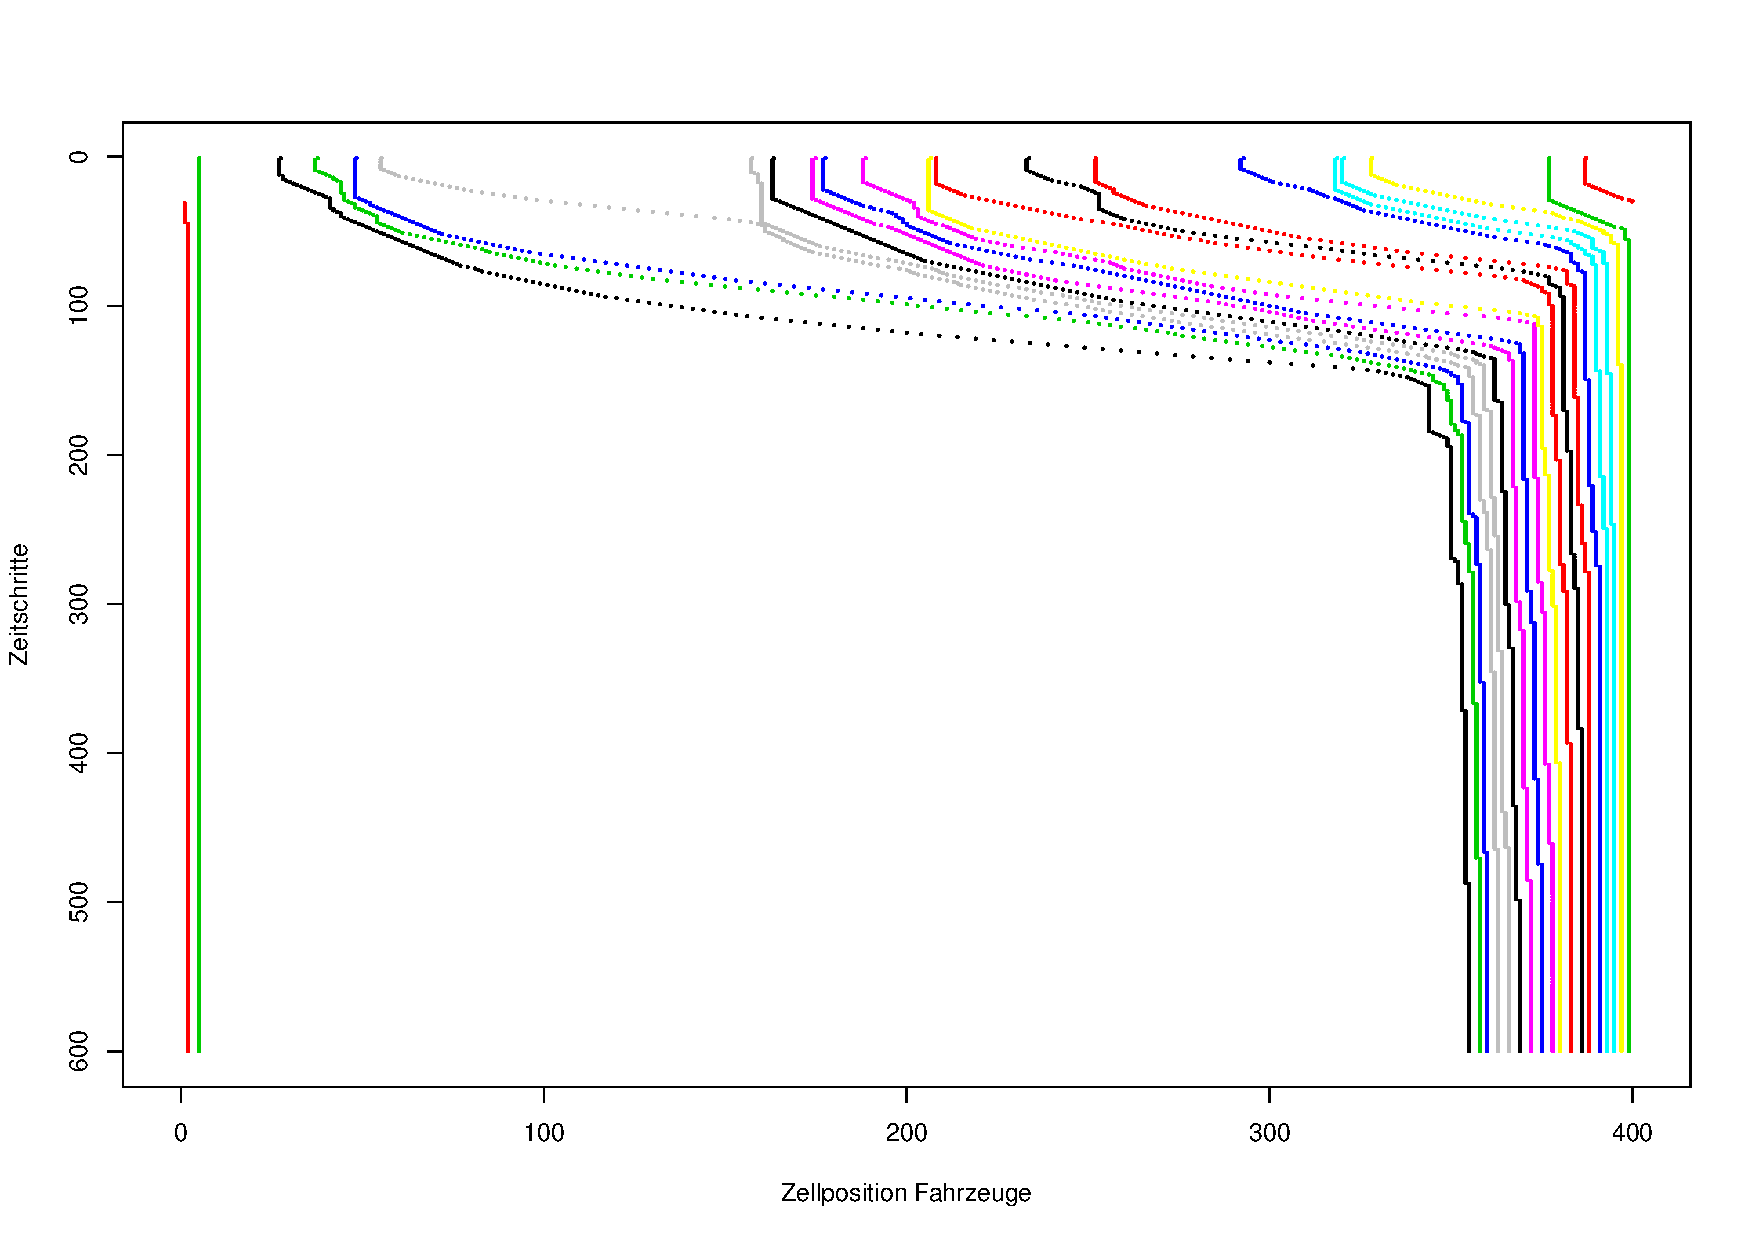
\includegraphics[width=0.45\textwidth]{go-negative_release-v185_success}\label{figure:go-negative-success}}
  \caption[Fehlerbehebung: Übergang vom Streckenende zum Anfang]
          {Fehlerbehebung des Übergangs vom Streckenende zum Anfang}
  \label{figure:go-negative}
\end{figure}

Durch Testläufe unterschiedlicher Versionen der Simulationssoftware mit identischen Szenariovorgaben - ein Fahrzeug wurde mit einer so kleinen Geschwindigkeit generiert, dass es in seiner Startzelle verblieb - konnte die Behebung des Fehlverhaltens nachgewiesen werden, siehe \cref{figure:go-negative}.

Danach konnten dann auch Stauwellen beobachtet werden, die sich rückwärts vom Streckenanfang her darüber hinaus am Streckenende fortsetzten. \sa{own: Stauwellenbild in Anhang, JSON 09mar 13:13}



\subsubsection{Unterteilung des Sichtfeldes der Fahrzeuge}
\label{sec:unterteilung-sichtfeld}

Um die relative Position eines anderen Fahrzeugs in der Umwelt festzustellen, kann die Richtung, in der dieses sich befindet, bestimmt werden.
Die Simulationssoftware hatte für das Sichtfeld der Fahrzeuge eine Unterteilung in acht Sektoren vorgesehen, sodass neben den Richtungen vorwärts, rückwärts, links und rechts auch Unterscheidung in Zwischenschritte links vorwärts, rechts vorwärts usw. möglich war, siehe \cref{figure:car-view-8sectors}.

\begin{figure}[hptb]
  \centering 
   \subfigure[acht Sektoren]{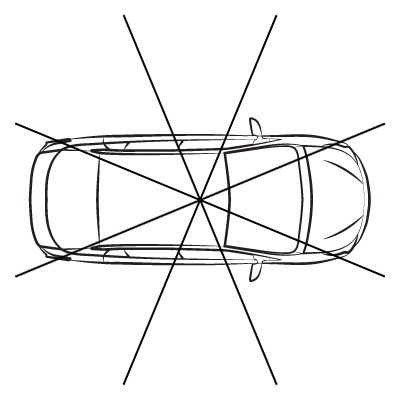
\includegraphics[width=0.3\textwidth]{car-view-8sectors}\label{figure:car-view-8sectors}}\qquad 
   \subfigure[zwei Sektoren]{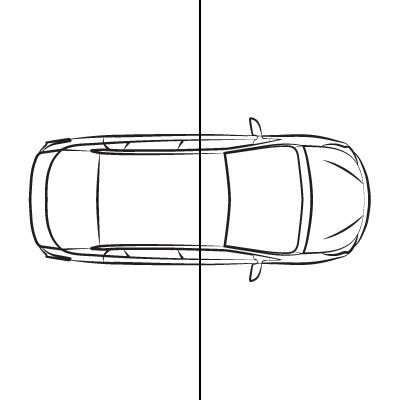
\includegraphics[width=0.3\textwidth]{car-view-2sectors}\label{figure:car-view-2sectors}}\qquad 
   \subfigure[vier Sektoren]{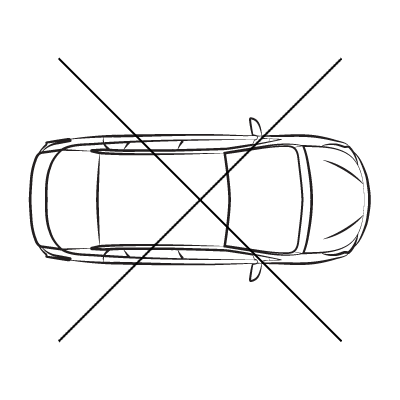
\includegraphics[width=0.3\textwidth]{car-view-4sectors}\label{figure:car-view-4sectors}}
  \caption[mögliche Unterteilung des Sichtfeldes]
          {mögliche Unterteilung des Sichtfeldes}
          {\footnotesize Quelle Auto-Silhouette: vecteezy.com} 
  \label{figure:car-view-sectors}
\end{figure}

Eine solch feine Unterscheidung war nicht nötig.
Es sollte genügen, feststellen zu können, ob sich ein anderes Fahrzeug relativ zum betrachteten Fahrzeug im vorwärtigen oder rückwärtigen Raum befindet, siehe \cref{figure:car-view-2sectors}. 
Die Abdeckung der Umwelt sollte dabei ohne Unterbrechung sein, d.h. jeder Position sollte einem der beiden Bereiche zugewiesen werden können.
Für die Simulation nach dem Einspurmodell von Nagel-Schreckenberg funktionierte dies ohne Probleme.

Bei einem Testlauf des Mehrspurmodells mit vier Fahrzeugen kam es allerdings zur Kollision zweier Fahrzeuge. 
Bei der Kontrolle des Logs wurde festgestellt, dass ein Fahrzeug (\texttt{vehicle0}), welches sich auf der Überholspur (lane 2) befand, ein anderes Fahrzeug (\texttt{vehicle20}) direkt neben sich nicht \enquote*{gesehen} hatte. 
Erkennbar in der Zeile \enquote{\texttt{PIA1}}, die nur ausgelöst wurde, wenn sich keinerlei Verkehr im Sichtfeld des Fahrzeuges befindet.
Es gab in dieser Konstellation demnach keine Zuordnung dieser Position zu einer der beiden Bereiche.
Daraufhin, so wie es das Verhalten des Agenten vorsah, wurde zum nächsten Schritt (366) in die Hauptspur gewechselt. 
In diesem Zeitschritt kam es dann zum Auslösen des Kollisionsereignisses, da der Abstand zwischen \texttt{vehicle0} und \texttt{vehicle20} nicht ausreichend groß war, um das hintere Fahrzeug mit seiner aktuellen Geschwindigkeit die volle Strecke zu bewegen.

Anmerkung: Gleichzeitig reagierte \texttt{vehicle0} korrekt auf das Hindernis direkt vor sich und leitete für den folgenden Zeitschritt einen Überholvorgang ein.

\footnotesize\begin{verbatim}
--- step 365 ----------------
         vehicle20   in lane   1   in cell   333.0   @   74.21582362319865   kph
         vehicle2   in lane   1   in cell   282.0   @   129.99324819683062   kph
         vehicle0   in lane   2   in cell   333.0   @   99.94723620551235   kph
PIA1     vehicle0   sees no traffic at all -> Pull-in
         vehicle1   in lane   1   in cell   90.0   @   130.8321253026147   kph
--- step 366 ----------------
         vehicle20   in lane   1   in cell   4.0   @   74.21582362319865   kph
         vehicle2   in lane   1   in cell   289.0   @   131.11124225593747   kph
         vehicle0   in lane   1   in cell   3.0   @   100.80986539456516   kph
TFC100   vehicle0   has vehicle in-front of -> decelerate
COS      vehicle0   STOPPED -> collision
OUT      vehicle0   -> Pull-out attempt successful
         vehicle1   in lane   1   in cell   97.0   @   130.64144521630223   kph
\end{verbatim}
\normalsize

Das Sichtfeld der Fahrzeuge wurde hierauf zu einem Vier-Sektoren-Modell abgewandelt, siehe \cref{figure:car-view-4sectors}, und die Pläne für Ein- und Ausscheren, der hiervon gleichermaßen betroffen sein dürfte, angepasst.
Es werden nun jeweils die beiden Sektoren kontrolliert, die die Bewegungs- bzw. Orientierungsrichtung darstellen. 
Nach vorn und hinten wird jeweils auch auf Entfernungen geprüft, seitlich genügt es auf reine Präsenz/Nichtpräsenz von anderen Fahrzeugen zu prüfen.

Im Rahmen dieser Umstellung wurde festgestellt, dass es bei der Richtungsbestimmung einen weiteren Fehler in der Simulationssoftware gab.
Die Berechnung lieferte für beide seitlichen Richtungen ein und denselben Wert und somit auch die gleiche Blickrichtung.
Der Fehler war durch die Verwendung der Methode \texttt{acos} entstanden, wobei nicht beachtet wurde, dass der \textit{arccos} nur im Bereich 0 bis $ \pi $ definiert ist, hier aber der Vollkreis zugrunde liegt.





\subsection{Setups für die Langzeittests}
\label{sec:setup-dauertests}

Für die Durchführung der Dauersimulationen galt es sinnvolle Einstellungen zu finden. 
Für das Agentenverhalten wurde dies in \cref{sec:verfeinerung-agentenplan} beschrieben. 
Nachfolgend sind Festlegungen für das Szenario zu finden.



\subsubsection{Fahrzeuganzahl}
\label{sec:fahrzeuganzahl}

Um einen Anhaltspunkt für die Anzahl der zu simulierenden Fahrzeuge zu erhalten, wurden reale Daten der Bundesanstalt für Straßenwesen aus dem Jahr 2016 für je eine automatische Dauerzählstelle auf den Autobahnen A7\footnote{siehe \url{http://www.bast.de/DE/Verkehrstechnik/Fachthemen/v2-verkehrszaehlung/Daten/2016_1/Jawe2016.html?nn=626916&cms_detail=4602&cms_map=0}, abgerufen am 09. März 2018}, A38\footnote{siehe \url{http://www.bast.de/DE/Verkehrstechnik/Fachthemen/v2-verkehrszaehlung/Daten/2016_1/Jawe2016.html?nn=626916&cms_detail=4372&cms_map=0}, abgerufen am 09. März 2018} und A71\footnote{siehe \url{http://www.bast.de/DE/Verkehrstechnik/Fachthemen/v2-verkehrszaehlung/Daten/2016_1/Jawe2016.html?nn=626916&cms_detail=4340&cms_map=0}, abgerufen am 09. März 2018} in der Harzregion herangezogen, siehe \cref{tab:reale-verkehrsdaten}. 
Das Teilstück auf der A7 war zu dieser Zeit nur zweispurig ausgebaut. 
Die A38 und die A71 sind generell nur zweispurig.
\\
Für eine Messstelle auf der A395 zwischen Bad Harzburg und Braunschweig lagen nur Werte aus dem Jahr 2014 vor.
Die Zahlen lagen nur wenig über den aktuelleren der Messstelle auf der A38.
Aus diesem Grund wurde auf die Einbeziehung verzichtet.


\begin{table}[hptb]
\begin{center}
\setlength{\tabcolsep}{0.5em} % for the horizontal padding
{\renewcommand{\arraystretch}{1.2}% for the vertical padding
\begin{tabular}{| c  c  c  c |}
\hline 
Zählstelle & Düderode & Röstebachtalbrücke & Tunnel Schmücke \\
(Autobahn) & (A7) & (A38) & (A71) \\
\hline 
Lage zw. AS & Seesen (Harz) & Breitenworbis & Heldrungen \\
 & und Echte & und Leinefelde & und Kölleda \\
\hline 
Verkehr Fahrtrichtung 1 & 25.881 & 11.851 & 6.418 \\ 
\hline 
Verkehr Fahrtrichtung 2 & 26.340 & 11.877 & 6.386 \\ 
\hline 
Durchschnitt pro Tag & 26.111 & 11.864 & 6.402 \\ 
\hline 
Durchschnitt pro Stunde & 1.088 & 495 & 267 \\ \hline
\end{tabular}
}
\caption{durchschnittliche tägliche Verkehrsdaten}
\label{tab:reale-verkehrsdaten}
\end{center}
\end{table}

\noindent
Bei der Berechnung der Durchschnitte wurde, wenn nötig, auf volle Fahrzeuge aufgerundet.

Die o.a. Zahlen spiegeln eine Verkehrsstärke ($q$ in $ \frac{\text{Fahrzeuge}}{\text{Zeit}} $) wieder.
Nach \cite{verkehrsplanung} kann diese mit Hilfe der mittleren momentanen Geschwindigkeit ($\overline{v}_{m}$) in eine Verkehrsdichte ($\rho$ in $ \frac{\text{Fahrzeuge}}{\text{Streckenabschnitt}} $) umgerechnet werden.
Der Zusammenhang lautet: $ \rho = \frac{q}{\overline{v}_{m}} $.

Die weiteren Berechnungen erfolgten jeweils mit den Durchschnittswerten der beiden Fahrtrichtungen.
Als $\overline{v}_{m}$ wird für Pkw 120 km/h angenommen.
Somit ergibt sich auf diesen Autobahnstücken eine Verkehrsdichte von 9,066 $\frac{\text{Fahrzeugen}}{\text{km}}$ für die A7, 4,125 für die A38 und 2,225 für die A71.
\\
Aufgrund der Einspurigkeit muss dieser Wert für das Szenario halbiert werden. 
Die Anzahl der Fahrzeuge erhält man dann durch Multiplikation mit der Streckenlänge.
Die Rundung erfolgte zum nächsten ganzen Fahrzeug.

Ausgangswerte für die Simulation einer 7,5 km langen Strecke sind die folgenden Fahrzeuganzahlen: 
\begin{itemize}
	\itemsep0em
	\item 34 (A7)
	\item 15 (A38)
	\item 8 (A71)
\end{itemize}

\paragraph*{Anmerkung zum Teilstück auf der A7}
\hfill \\
Die Autobahn A7, im Bereich Niedersachsen, wurde in den vergangenen Jahren an vielen Stellen auf drei Spuren je Fahrtrichtung verbreitert.
Das Teilstück zwischen den Anschlussstellen Seesen und Nörten-Hardenberg war eines der letzten zweispurigen.
Der Umbau hat im September 2017 begonnen\footnote{siehe \url{https://www.strassenbau.niedersachsen.de/download/45795/Sechsstreifiger_Ausbau_der_A_7_Uebersichtskarte.pdf}, abgerufen am 09. März 2018}.
Mit seiner Lage zwischen zwei bereits dreispurig ausgebauten Teilstücken, mussten hier sicherlich größere Verkehrslasten bewältigt werden, als auf anderen zweispurigen Autobahnen.

Für die Simulation war dies ein glücklicher Zufall, da im speziellen $p_{linger}$ mit der hier vorgegebenen Fahrzeuganzahl weiter präzisiert werden konnte, siehe \cref{sec:adjust-linger}.




\subsubsection{Zellgröße und Zeitschrittgröße}
\label{sec:cellsize-timesteplength}

Den nachfolgenden Ausführungen liegt das hier beschriebene Szenario zugrunde:
\begin{itemize}
\itemsep0em
	\item Anzahl Lanes: 1
	\item Streckenlänge: 1 km
	\item Simulationsdauer: 30 min
	\item Anzahl Fahrzeuge: 2
	\item max. zulässige Geschwindigkeit: 100 km/h
	\item Trödelwahrscheinlichkeit: 0,1
\end{itemize}
Mit dem bereits erwähnten Vorgehen - identische Agentenpläne, unterschiedliches Geschwindigkeitsintervall bei der Initialisierung (schnelleres Fahrzeug (rote Kurve), $ v \in [80; 130] $, langsameres Fahrzeug (schwarze Kurve), $ v \in [70; 90] $) - wurde das Verhalten der Agenten, ausgehend von einer Zellgröße von 7,5 Metern (in 2,5 m-Schritten absteigend) und einer Zeitschrittgröße von 0,1 Minuten (jew. halbiert), in jew. drei Durchgängen getestet.

Für die Auswertung, ob eine Zellgröße/Zeitschrittlänge-Kombination für eine Simulationsdurchführung nutzbar ist, wurde der Ausdruck der Geschwindigkeiten der beiden Fahrzeuge über die Simulationszeit genutzt.


\paragraph*{Zellgröße 7,5 m}
\hfill \\
\begin{figure}[hptb]
  \centering 
   \subfigure[1. Durchlauf]{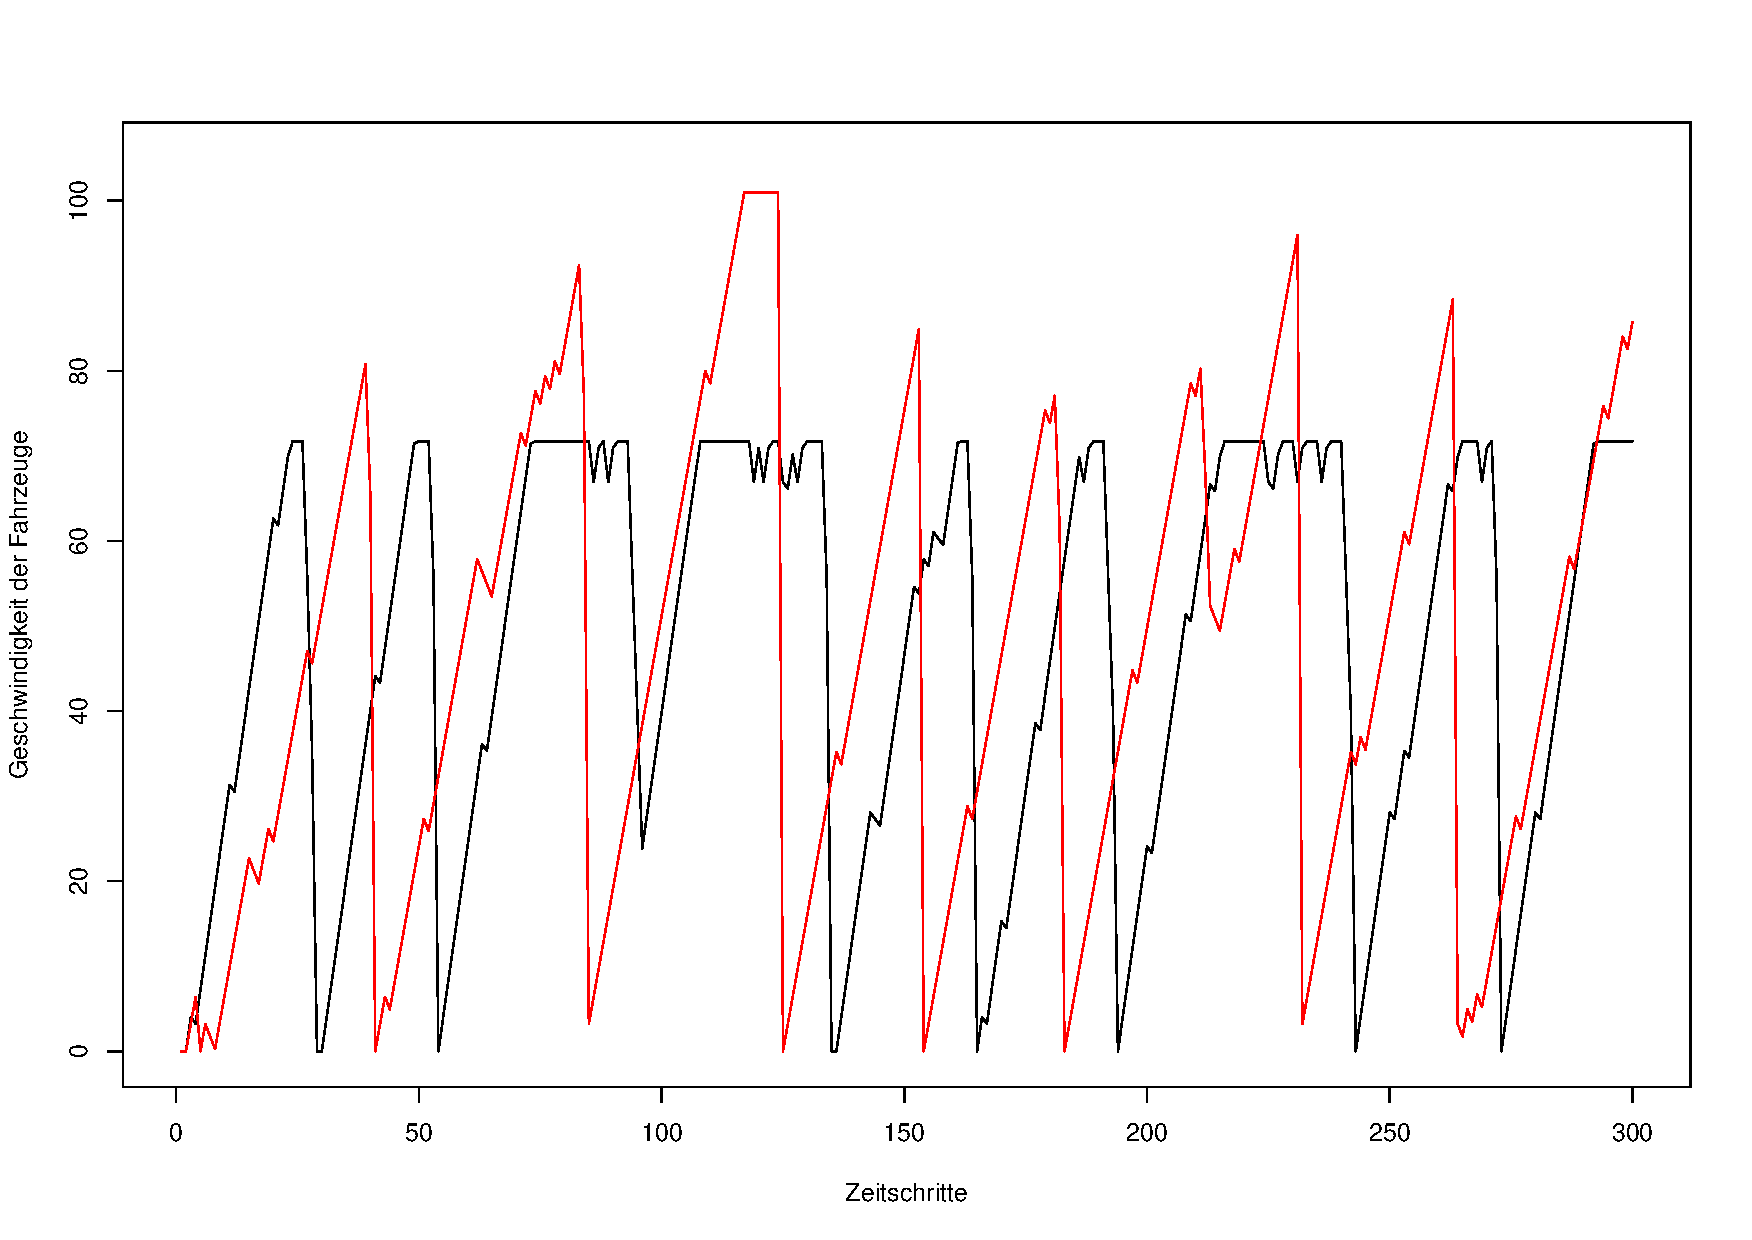
\includegraphics[width=0.3\textwidth]{speed_run1}\label{figure:run1}}\qquad 
   \subfigure[2. Durchlauf]{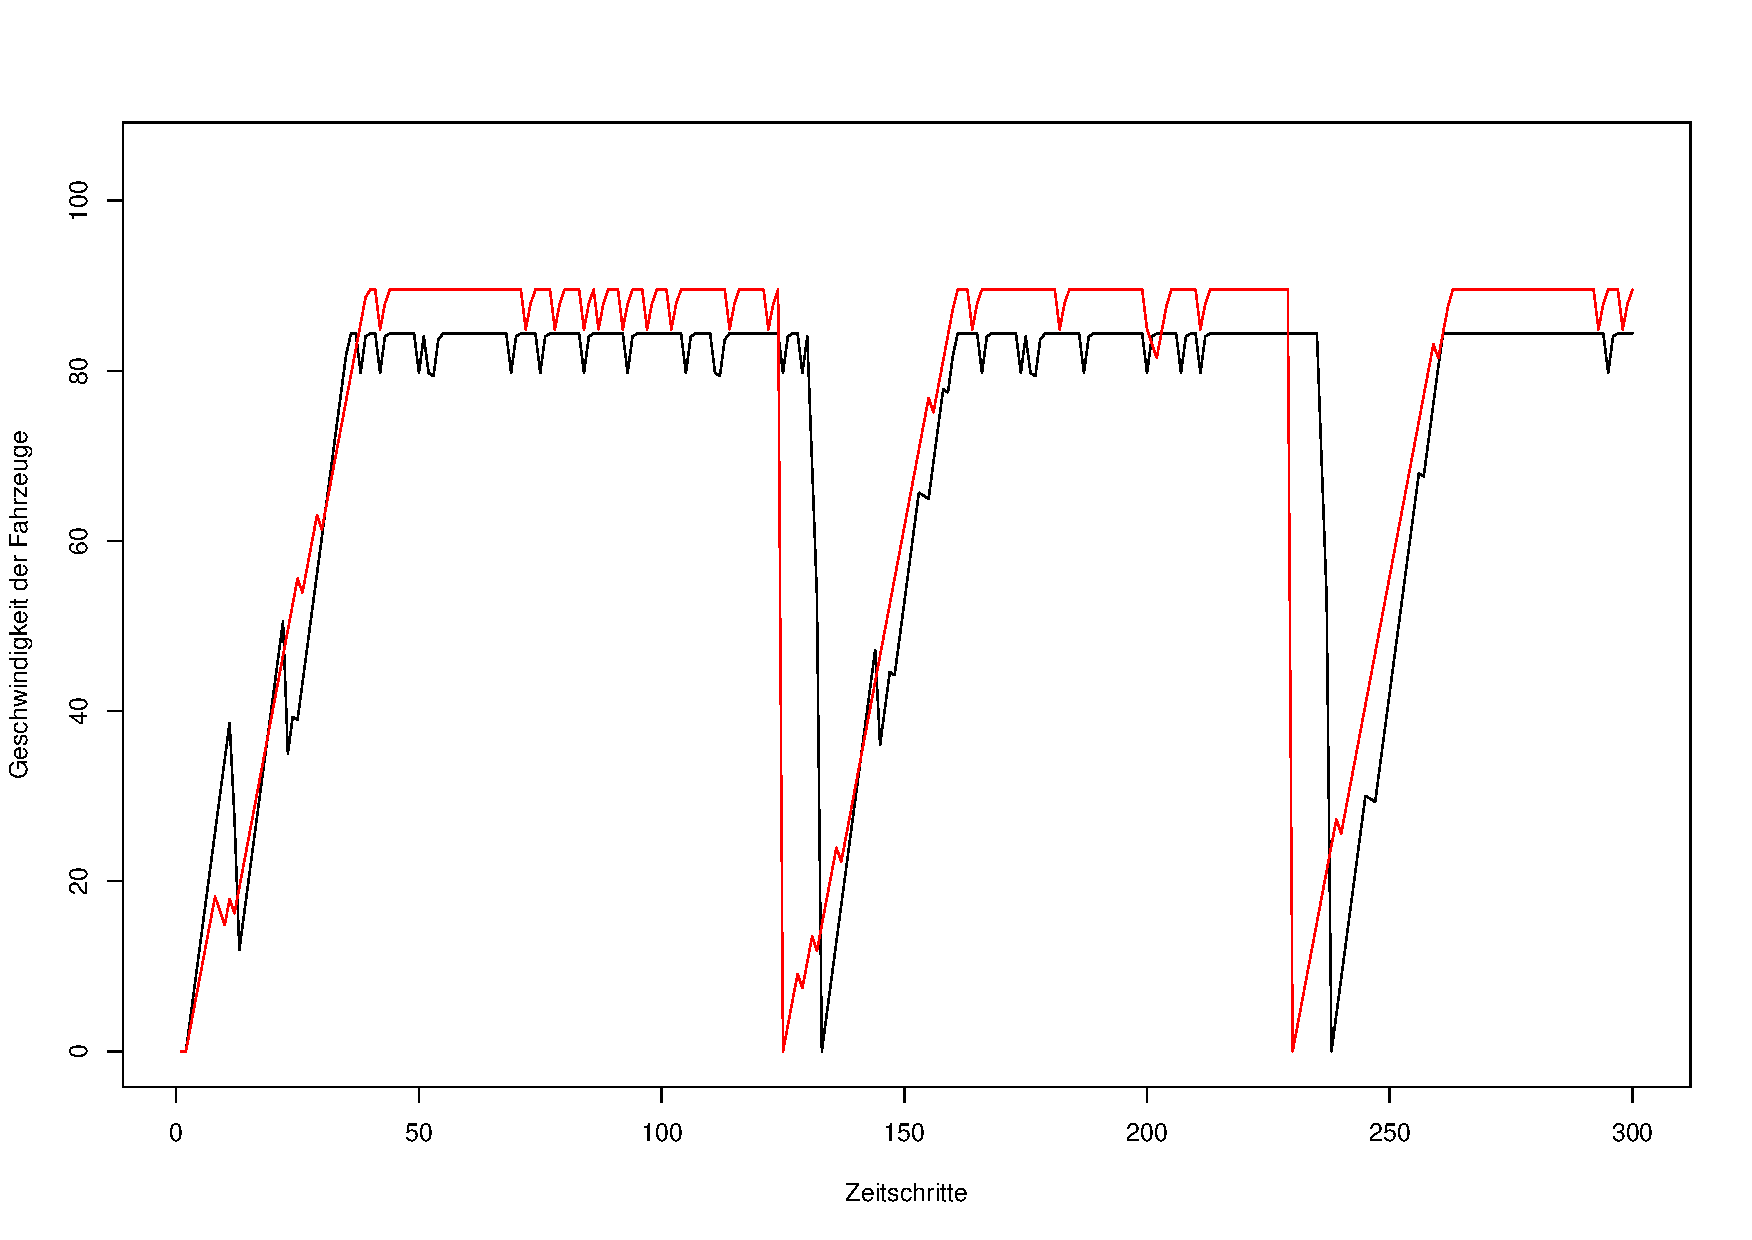
\includegraphics[width=0.3\textwidth]{speed_run2}\label{figure:run2}}\qquad 
   \subfigure[3. Durchlauf]{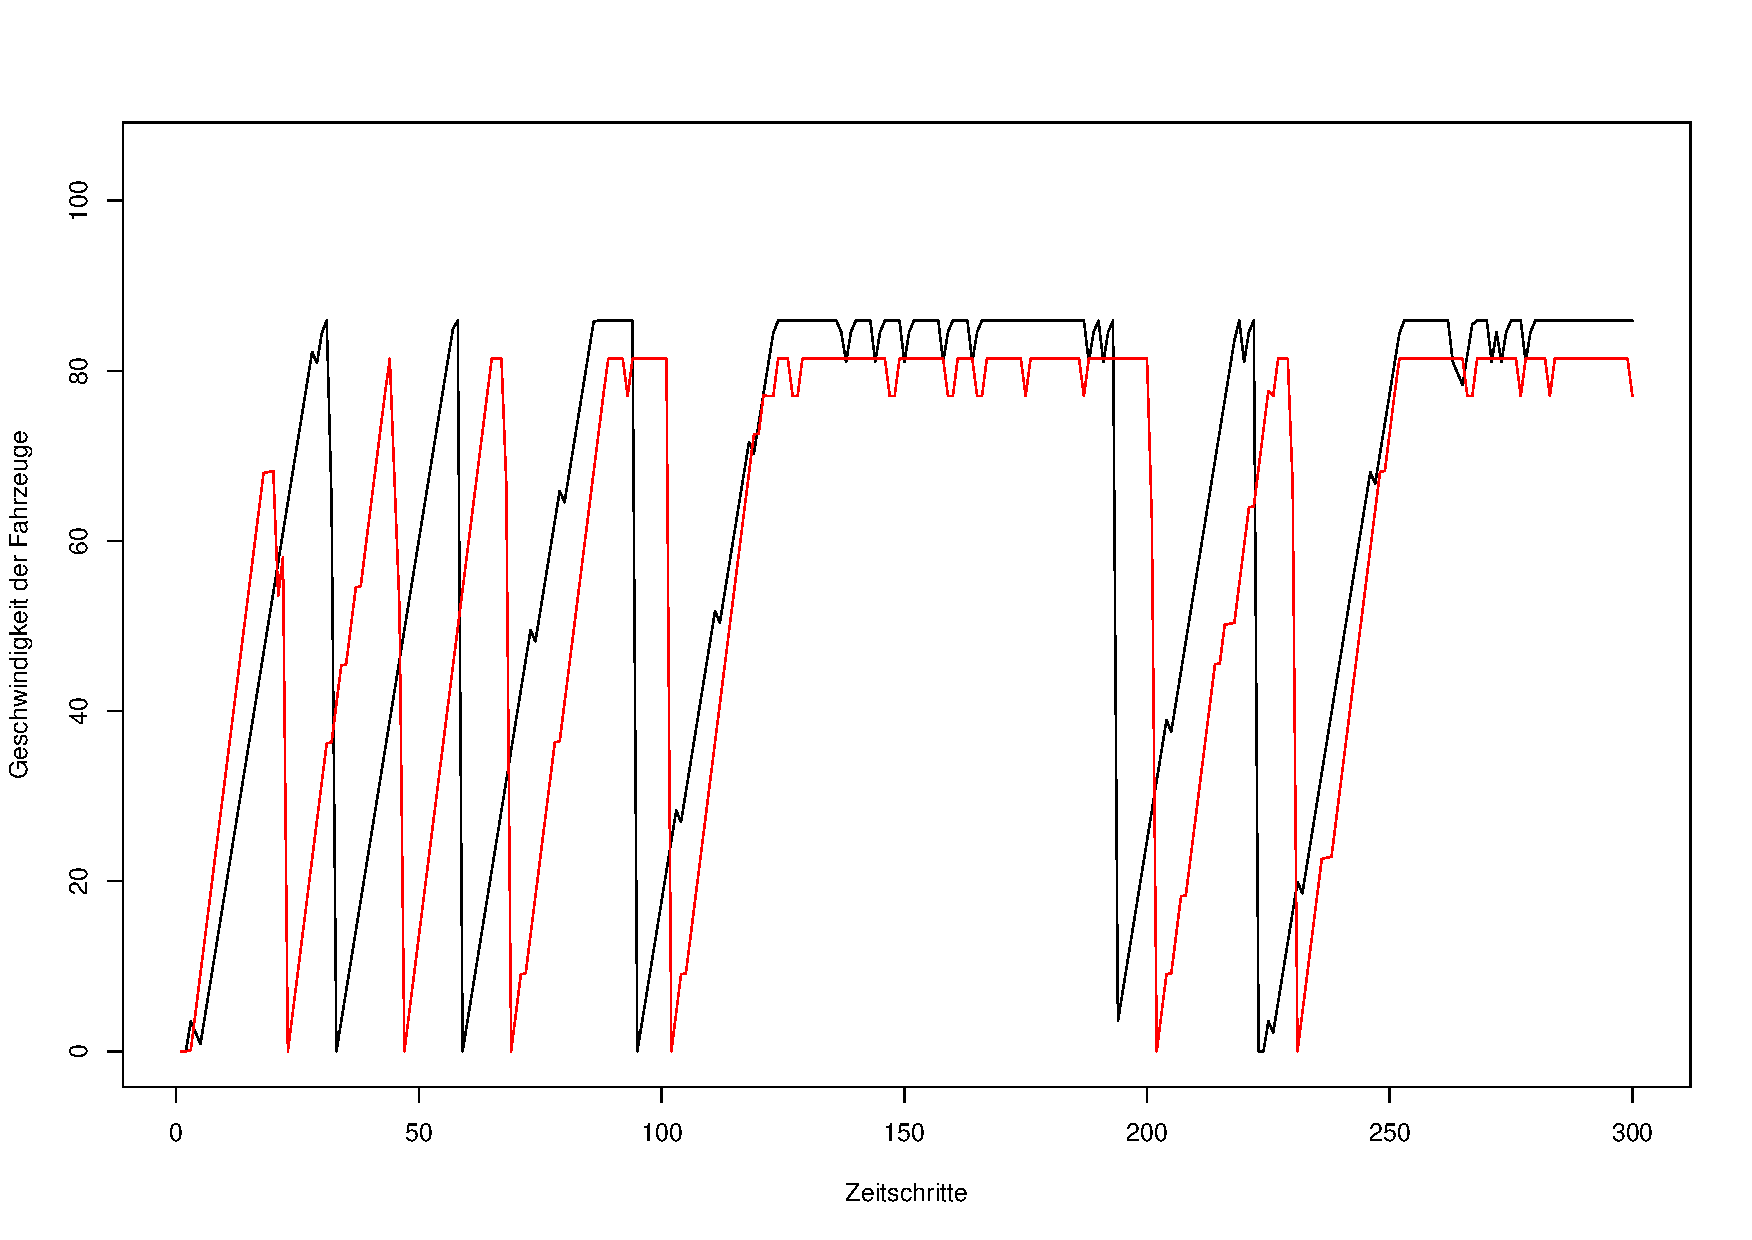
\includegraphics[width=0.3\textwidth]{speed_run3}\label{figure:run3}}
  \caption{Simulationen mit Zellgröße 7,5 m und Zeitschrittlänge 0,1 min} 
  \label{figure:run1-3}
\end{figure}

In allen drei Kurvenverläufen in \cref{figure:run1-3} sind mehrfach Reduktionen der Geschwindigkeit auf Null zu sehen. 
Dies zeigt, dass an diesen Stellen eine Kollision stattgefunden hat. Das Kollisionsereignis wird vom Simulationstool ausgelöst, wenn ein Fahrzeug nicht in der Lage wäre, im nächsten Zeitschritt die für seine Geschwindigkeit entsprechende Streckenlänge zurückzulegen.

Die Zeitschrittlänge von 0,1 Minuten, was sechs Sekunden entspricht, ist nicht ausreichend, um Geschwindigkeit in ausreichendem Maße abzubauen, um genug Abstand vom Vordermann einzuhalten.

Auf die Ausführung von Durchgängen mit dieser Zeitschrittgröße und kleinerer Zellgröße wurde verzichtet.

\begin{figure}[hptb]
  \centering 
   \subfigure[1. Durchlauf]{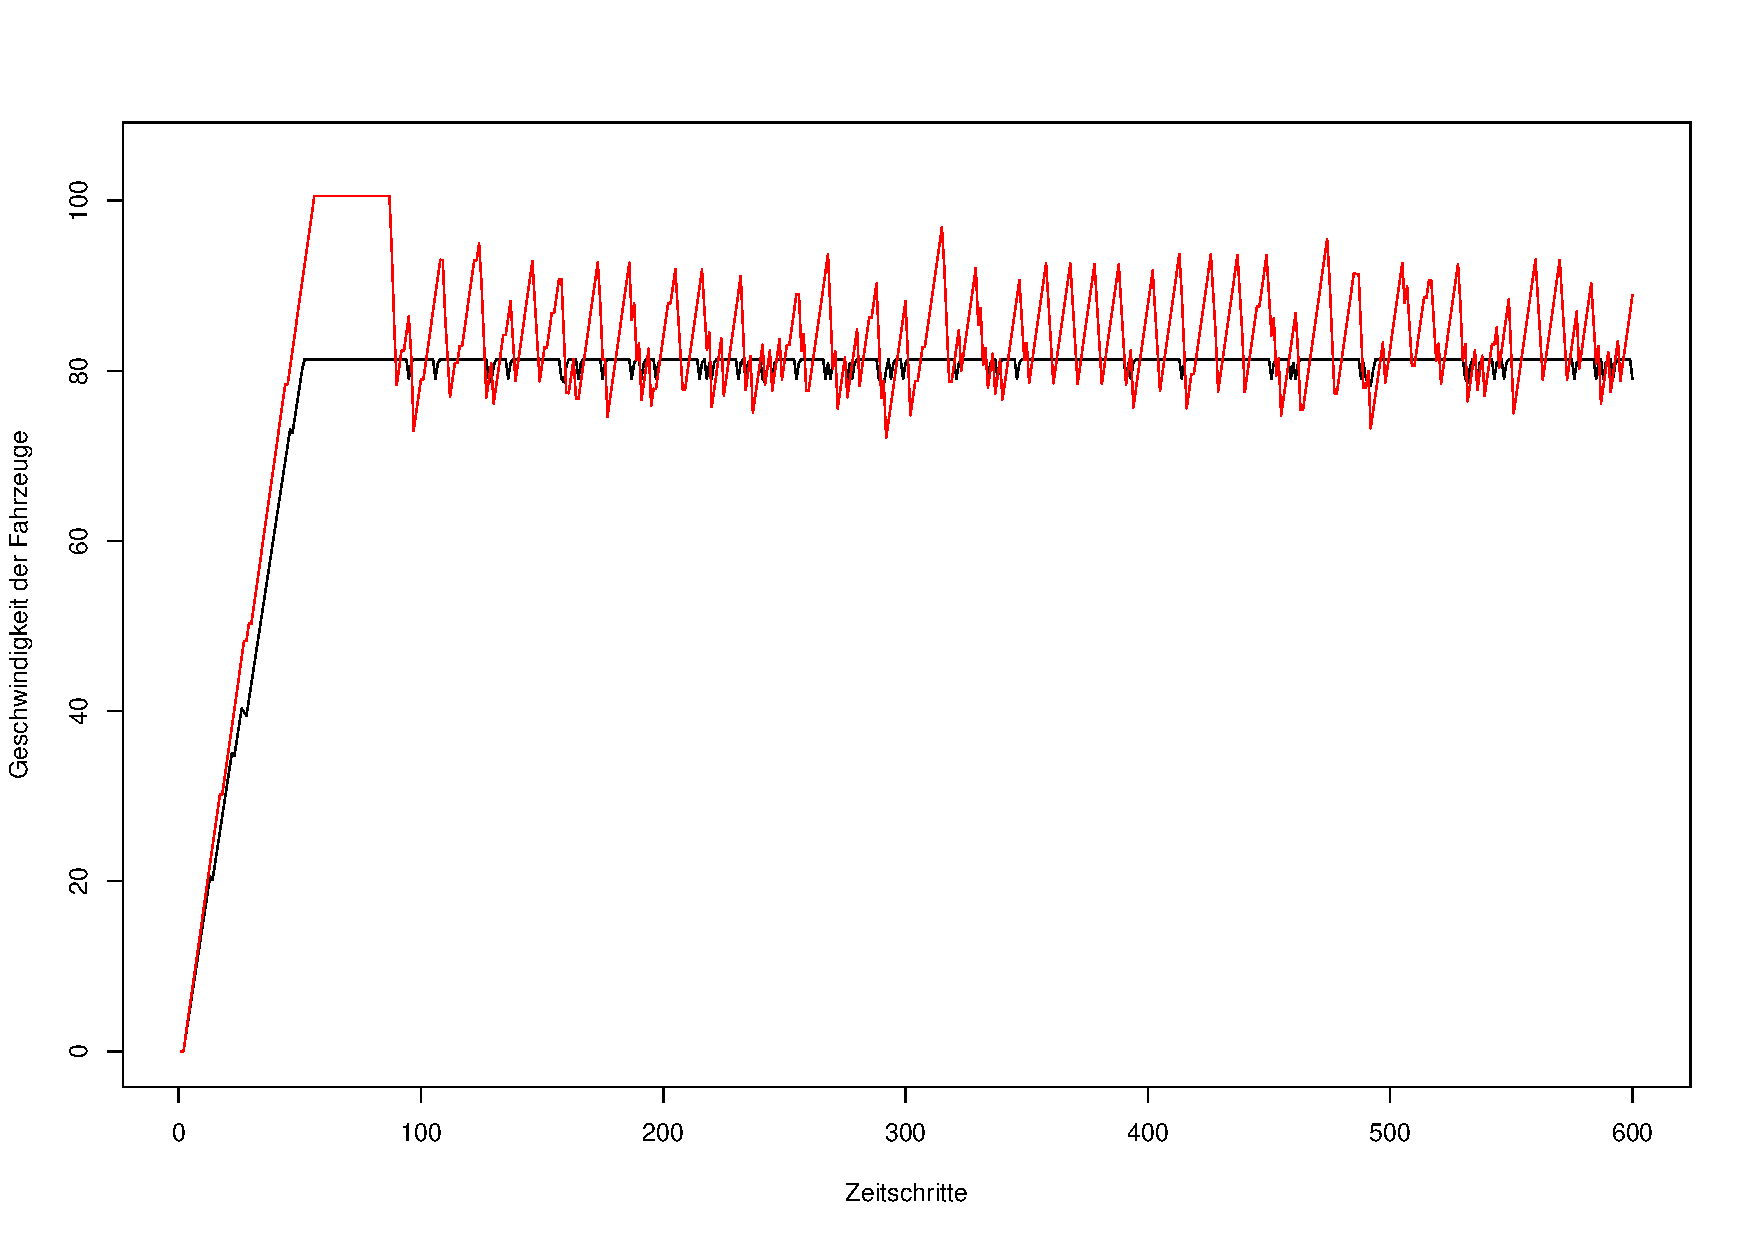
\includegraphics[width=0.3\textwidth]{speed_run4}\label{figure:run4}}\qquad 
   \subfigure[2. Durchlauf]{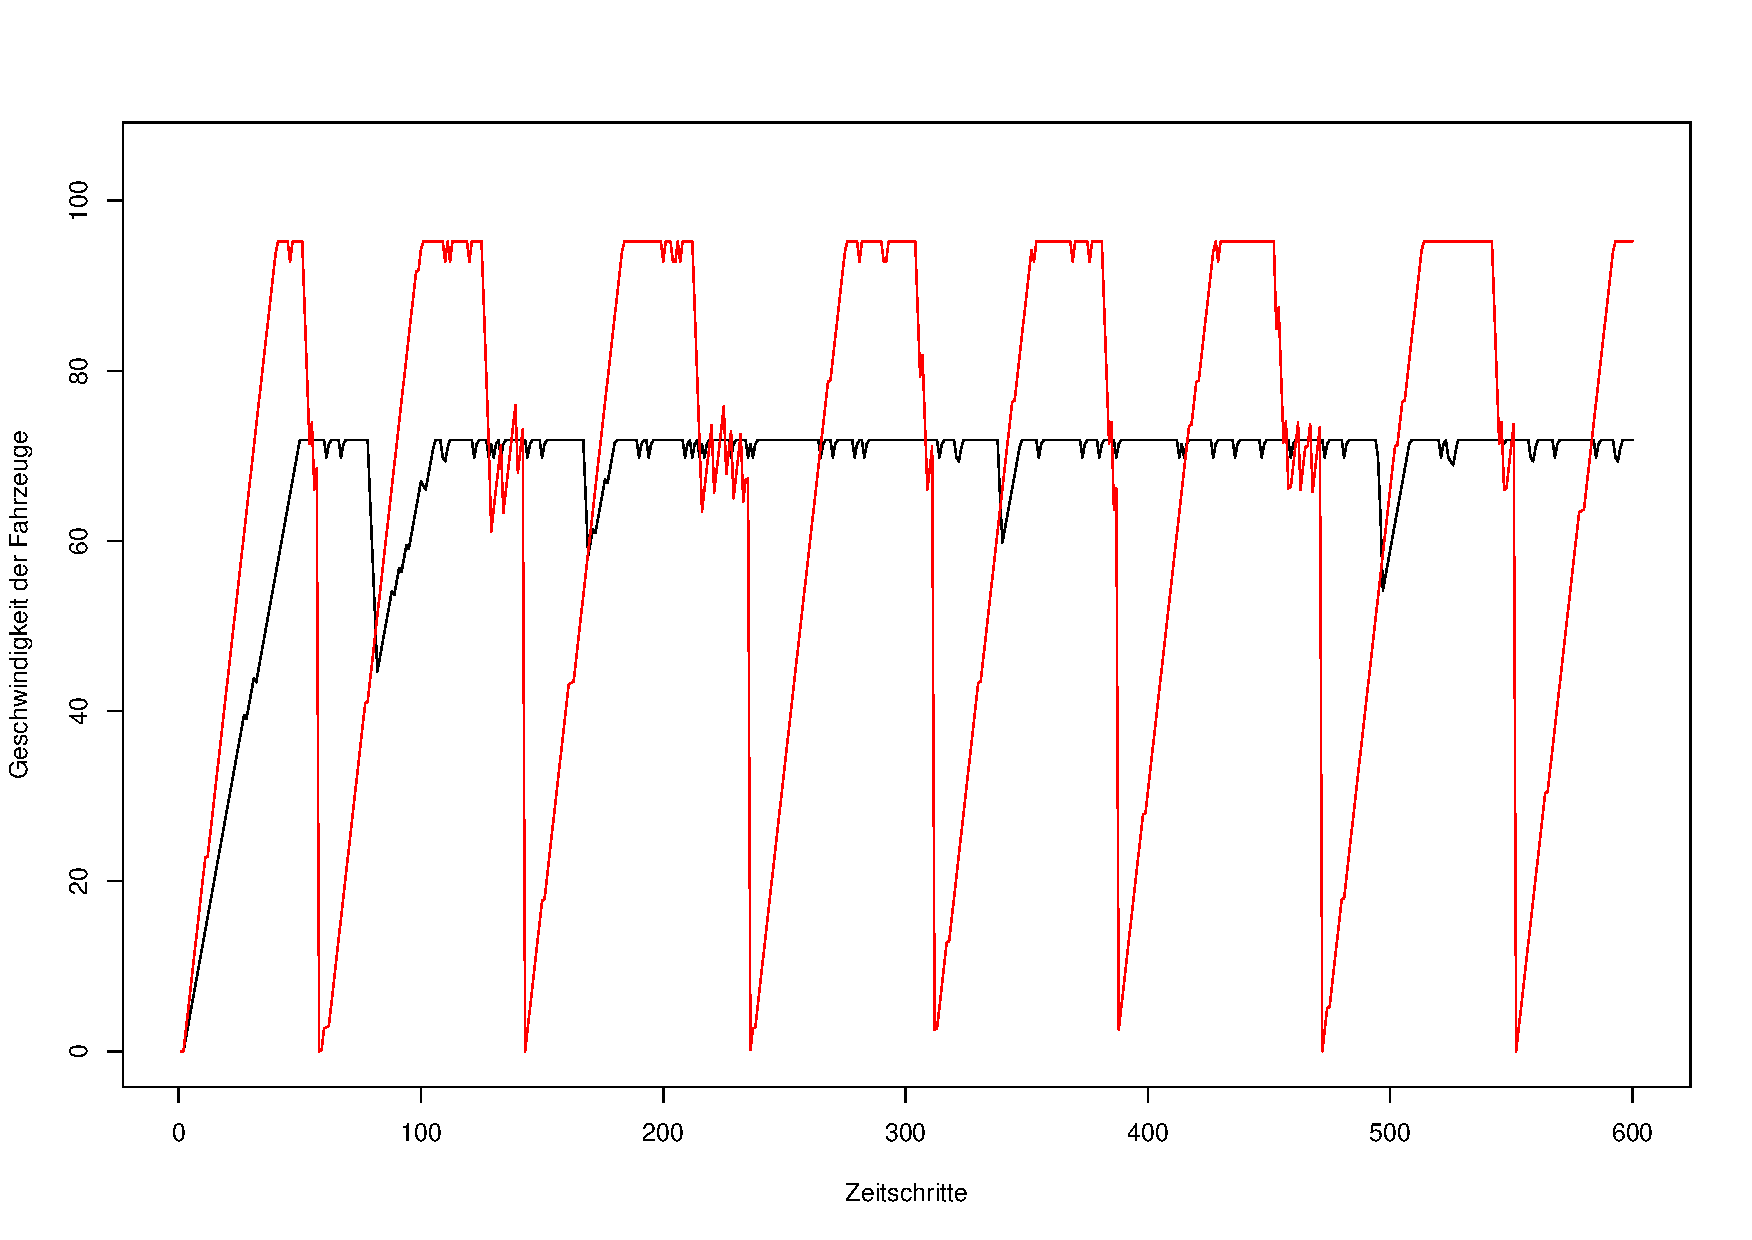
\includegraphics[width=0.3\textwidth]{speed_run5}\label{figure:run5}}\qquad 
   \subfigure[3. Durchlauf]{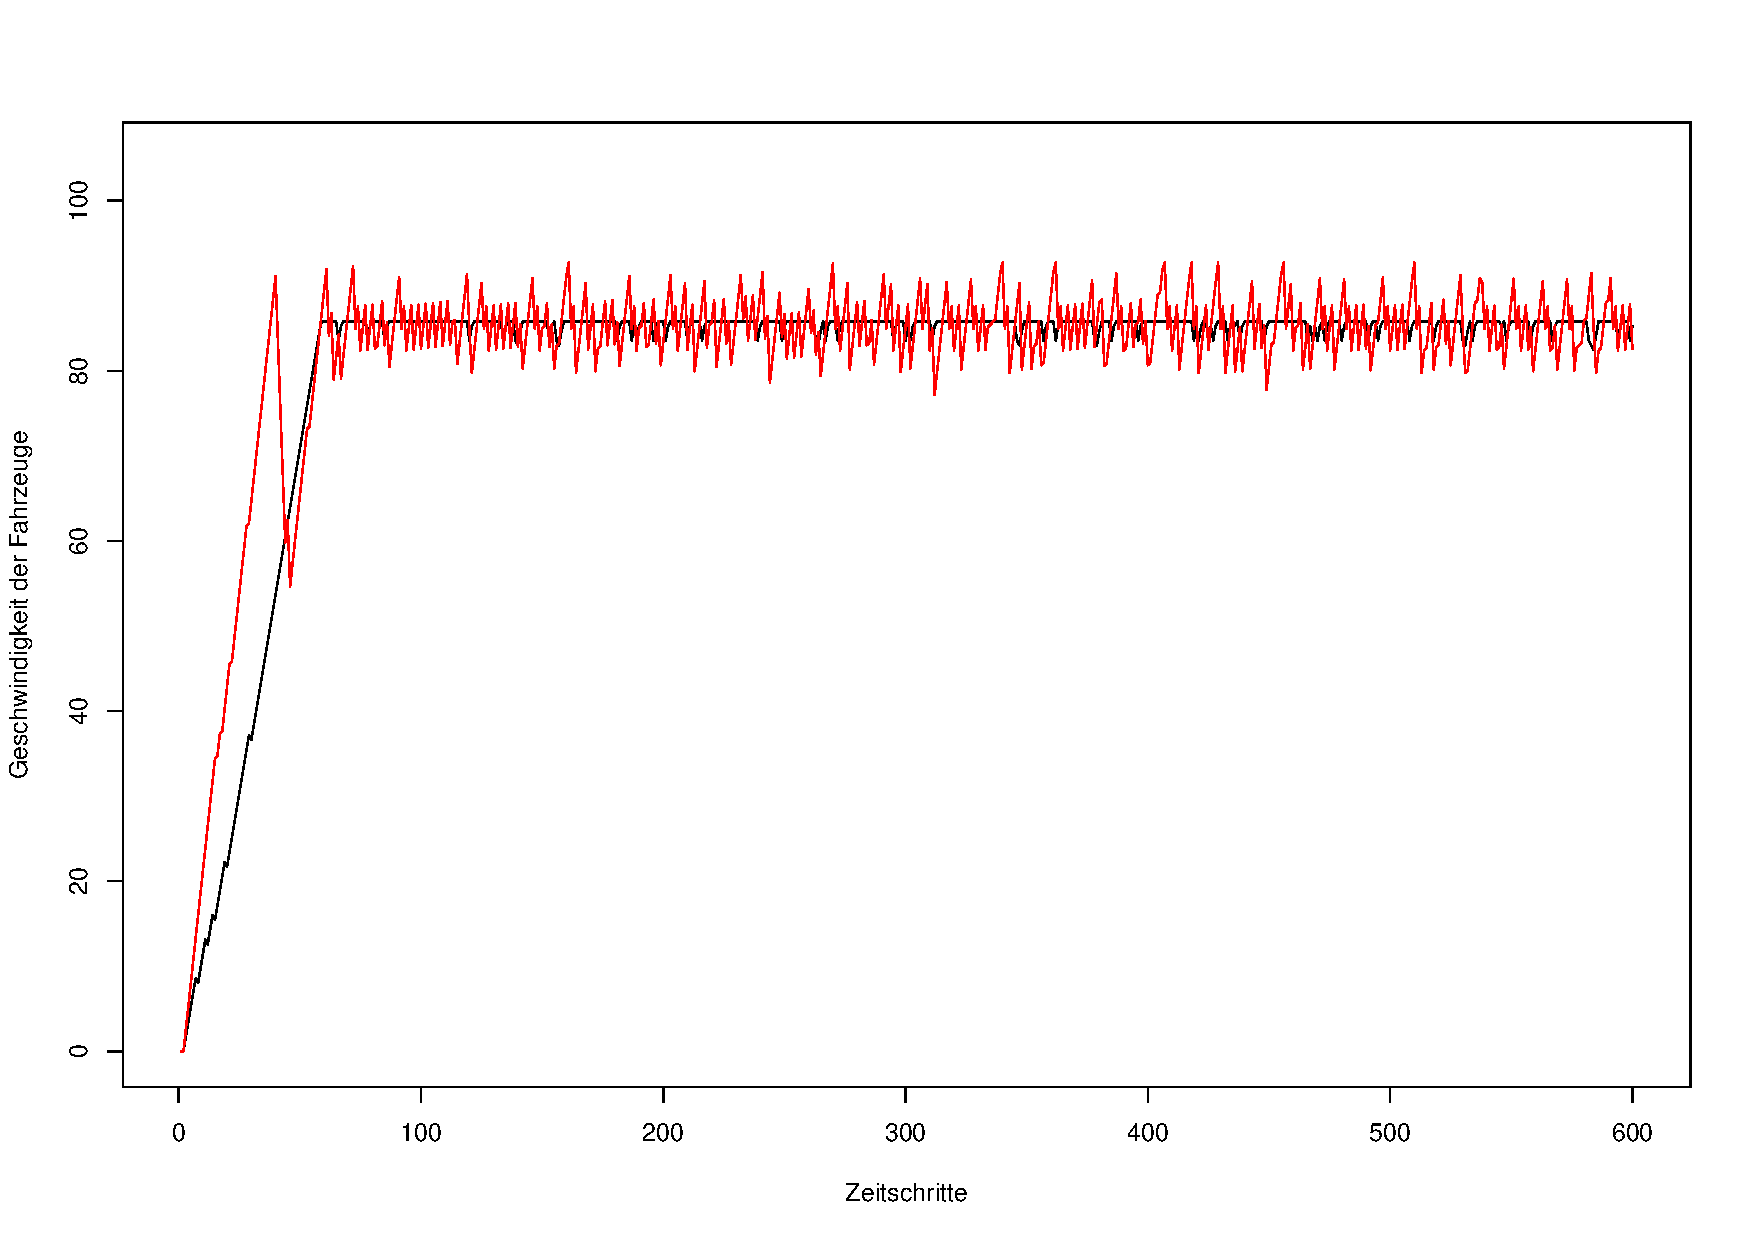
\includegraphics[width=0.3\textwidth]{speed_run6}\label{figure:run6}}
  \caption{Simulationen mit Zellgröße 7,5 m und Zeitschrittlänge 0,05 min} 
  \label{figure:run4-6}
\end{figure}

Die Verläufe der Kurven in \cref{figure:run4-6} zeigen in zwei von drei Fällen, dass sich die Geschwindigkeit des auffahrenden Fahrzeuges um die des langsameren Fahrzeuges einpendelt.

Im Plot des zweiten Durchlaufes ist zu sehen, dass auch in dieser Konstellation Kollisionen stattgefunden haben.
Die Geschwindigkeit des langsameren Fahrzeuges lag in diesem Durchlauf im Vergleich zu den anderen beiden um einiges niedriger.

\begin{figure}[hptb]
  \centering 
   \subfigure[1. Durchlauf]{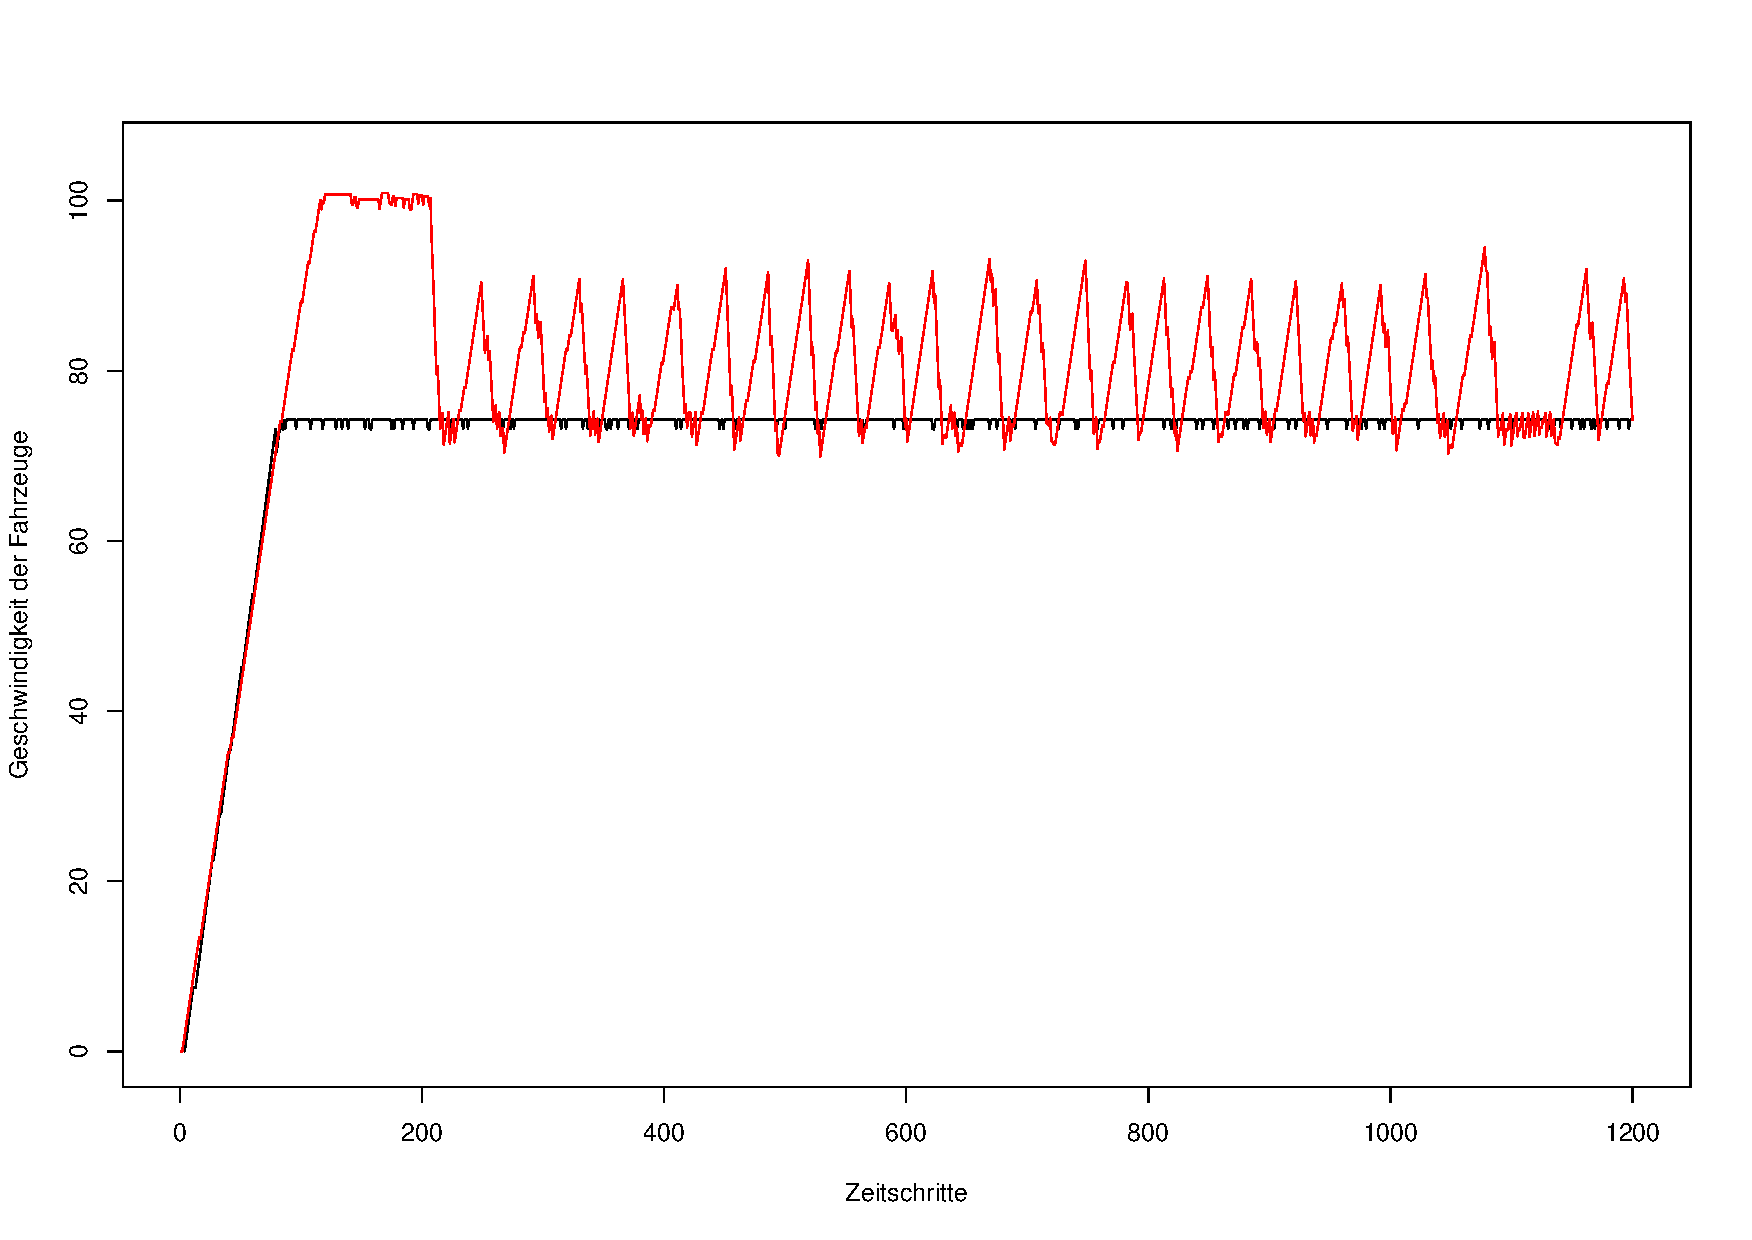
\includegraphics[width=0.3\textwidth]{speed_run7}\label{figure:run7}}\qquad 
   \subfigure[2. Durchlauf]{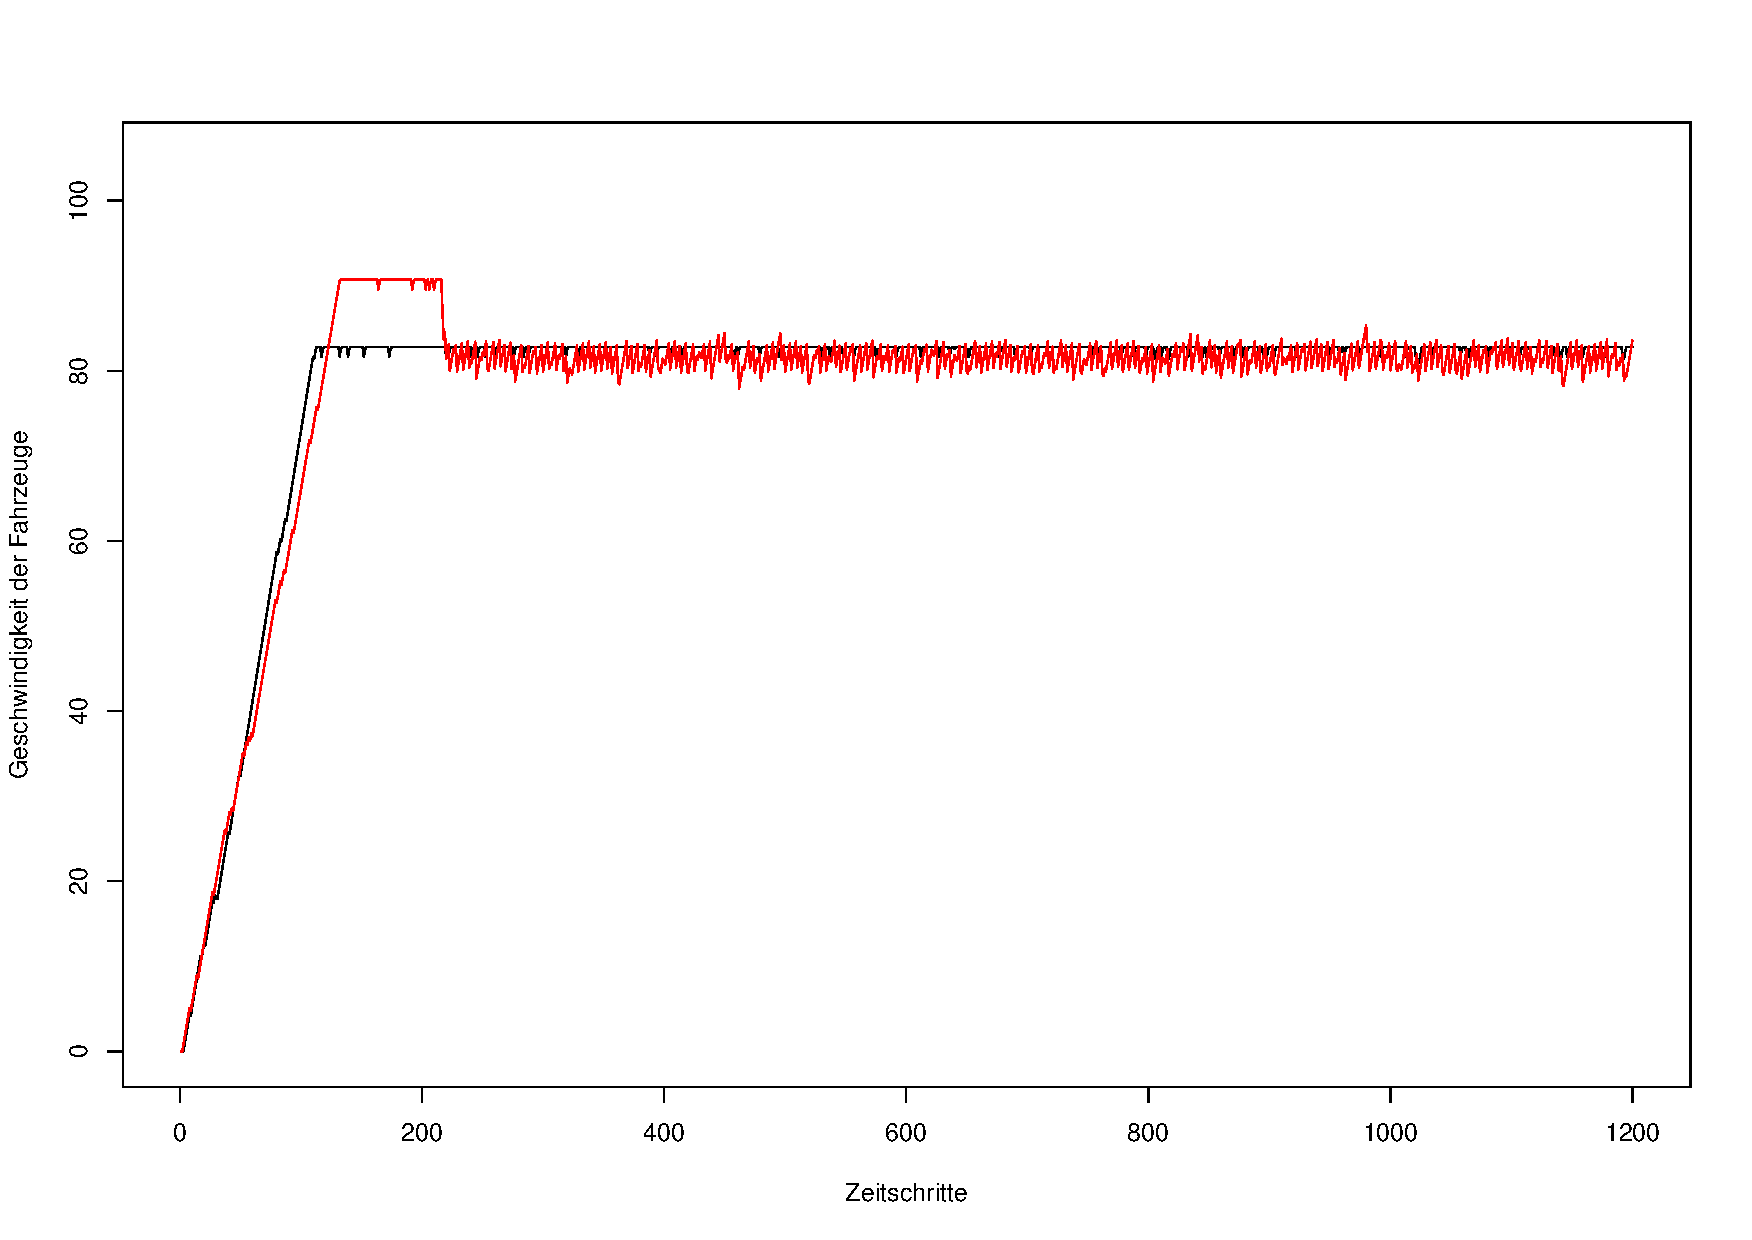
\includegraphics[width=0.3\textwidth]{speed_run8}\label{figure:run8}}\qquad 
   \subfigure[3. Durchlauf]{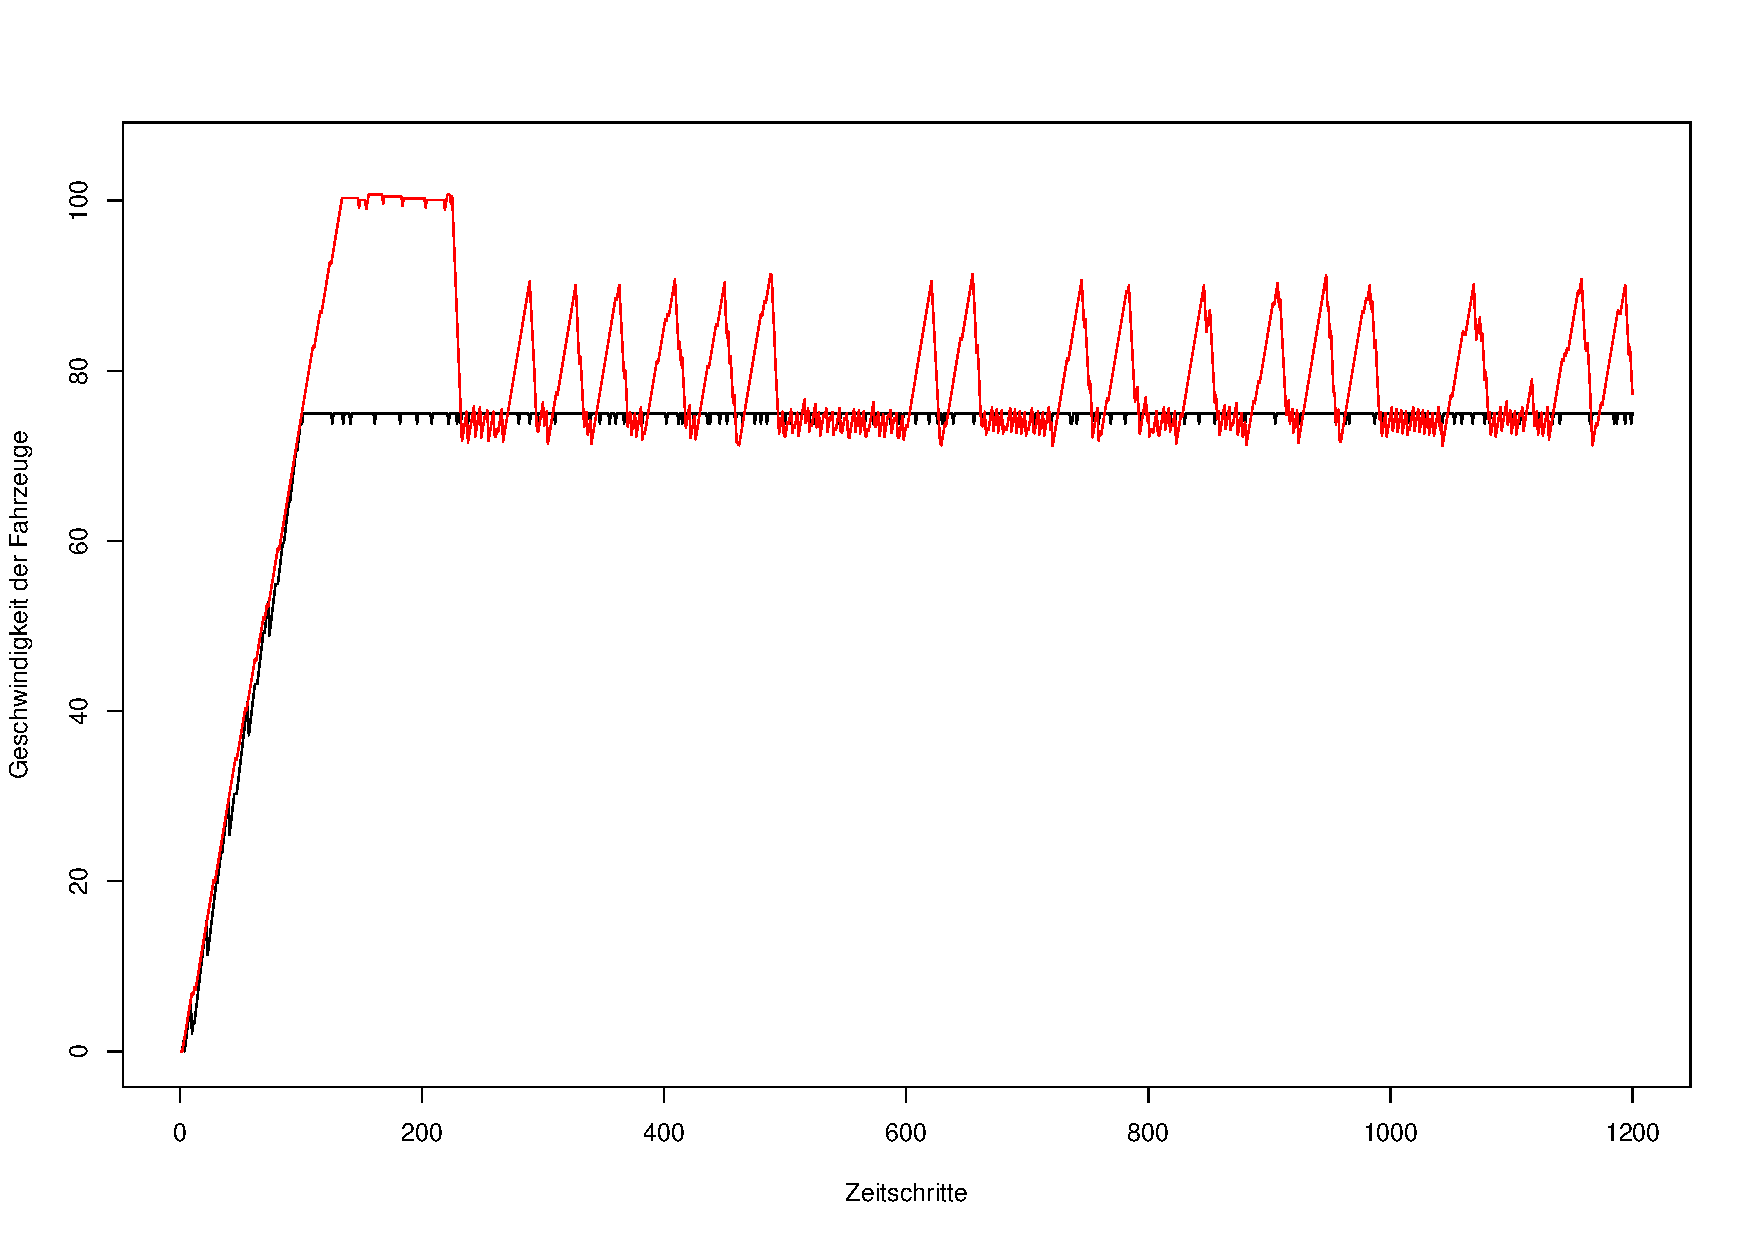
\includegraphics[width=0.3\textwidth]{speed_run9}\label{figure:run9}}
  \caption{Simulationen mit Zellgröße 7,5 m und Zeitschrittlänge 0,025 min} 
  \label{figure:run7-9}
\end{figure}

Die Geschwindigkeitskurve des schnelleren Fahrzeugs weist in \cref{figure:run7} ein sä"-ge"-zahn"-ähn"-liches Muster auf.
Dies resultiert aus den, im Vergleich zu den herbeigeführten Geschwindigkeitszuwächsen, großen Zellen.
Ein Geschwindigkeitsunterschied von zehn bis 15 km/h reicht bei entsprechend zugrunde liegender Ausgangsgeschwindigkeit nicht aus, eine Verkürzung des Abstands herbeizuführen.
Da sich die Abbrems- und Beschleunigungsmanöver identisch wiederholen, kommt es zu dieser Musterbildung.

Das Plot in \cref{figure:run8} zeigt ein Einordnen hinter dem langsameren Fahrzeug und die Beibehaltung von dessen Geschwindigkeit.
\cref{figure:run9} ist nahezu eine Mischform aus den ersten beiden Kurven.


\paragraph*{Zellgröße 5,0 m}
\hfill \\
\begin{figure}[hptb]
  \centering 
   \subfigure[1. Durchlauf]{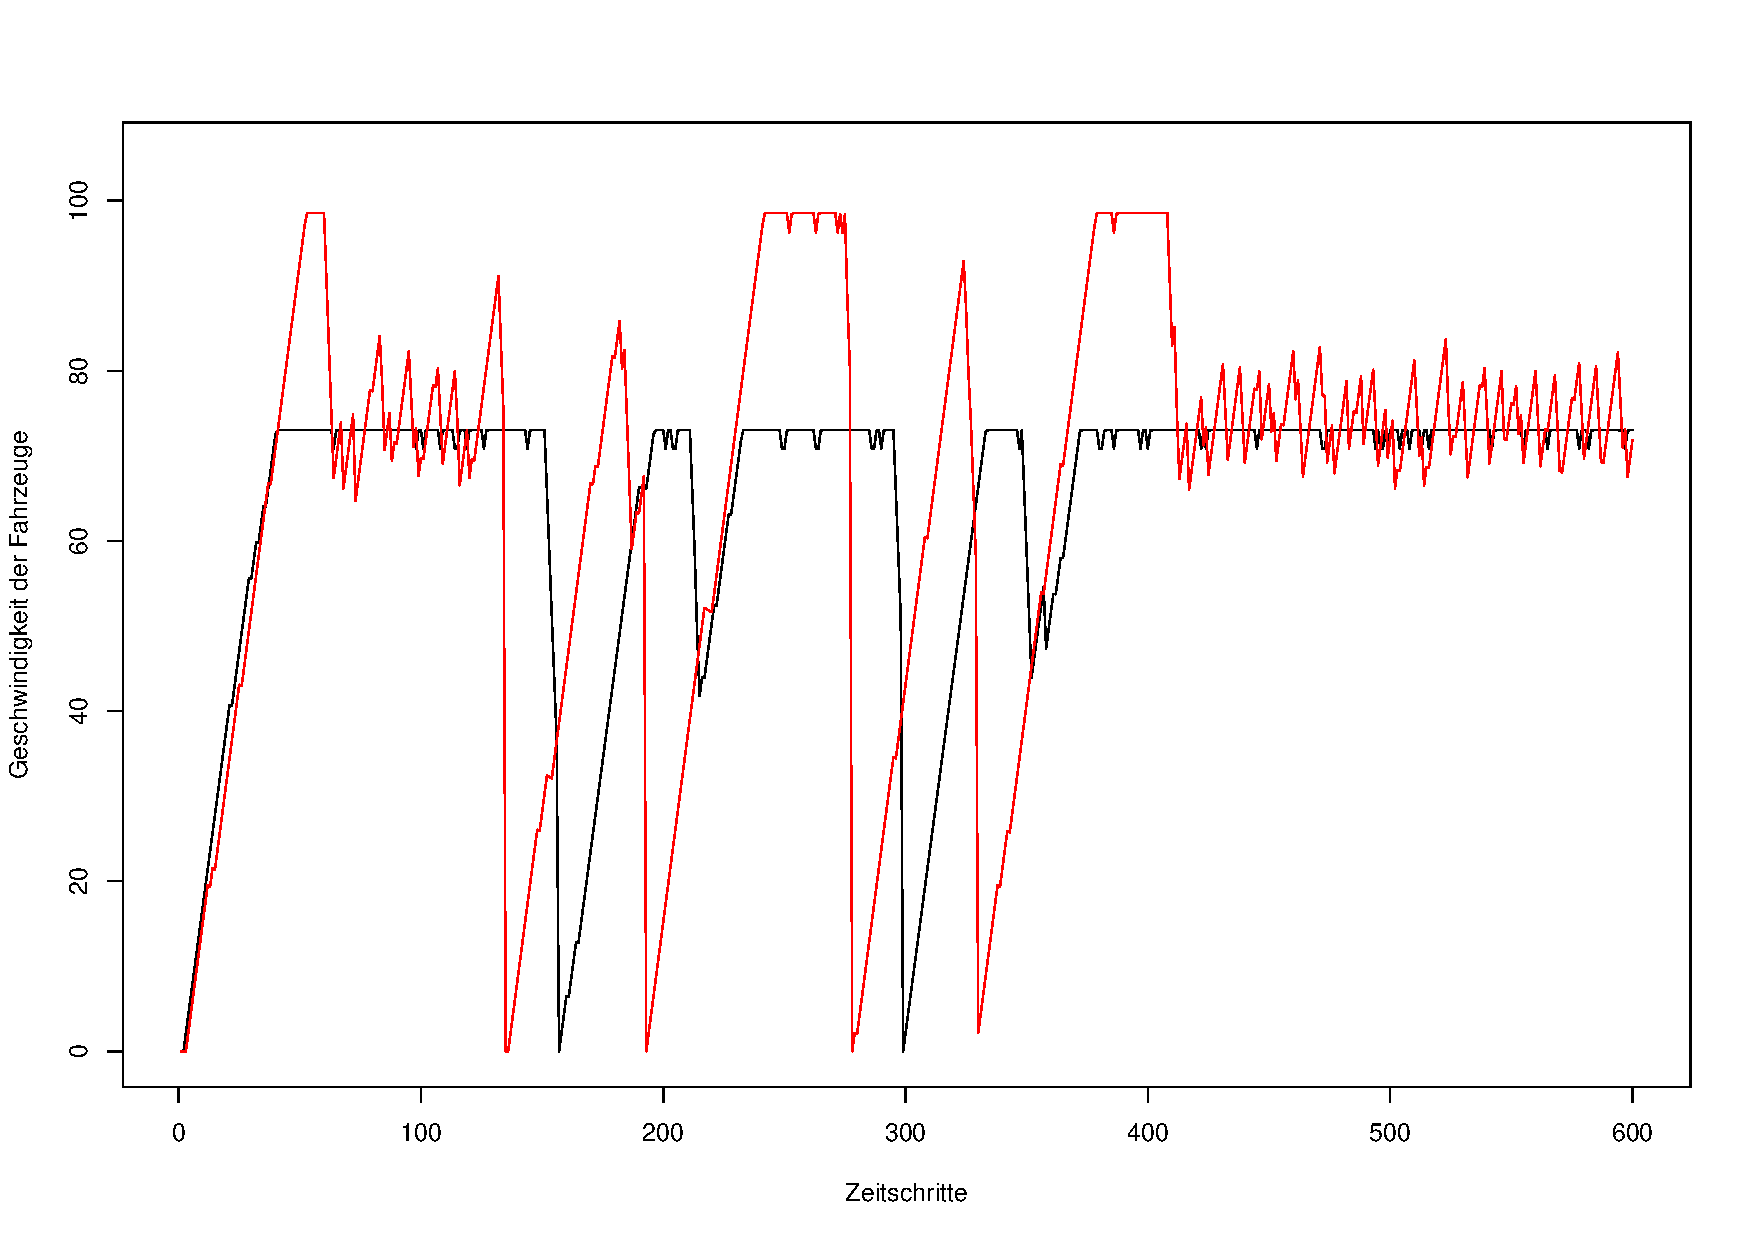
\includegraphics[width=0.3\textwidth]{speed_run14}\label{figure:run14}}\qquad 
   \subfigure[2. Durchlauf]{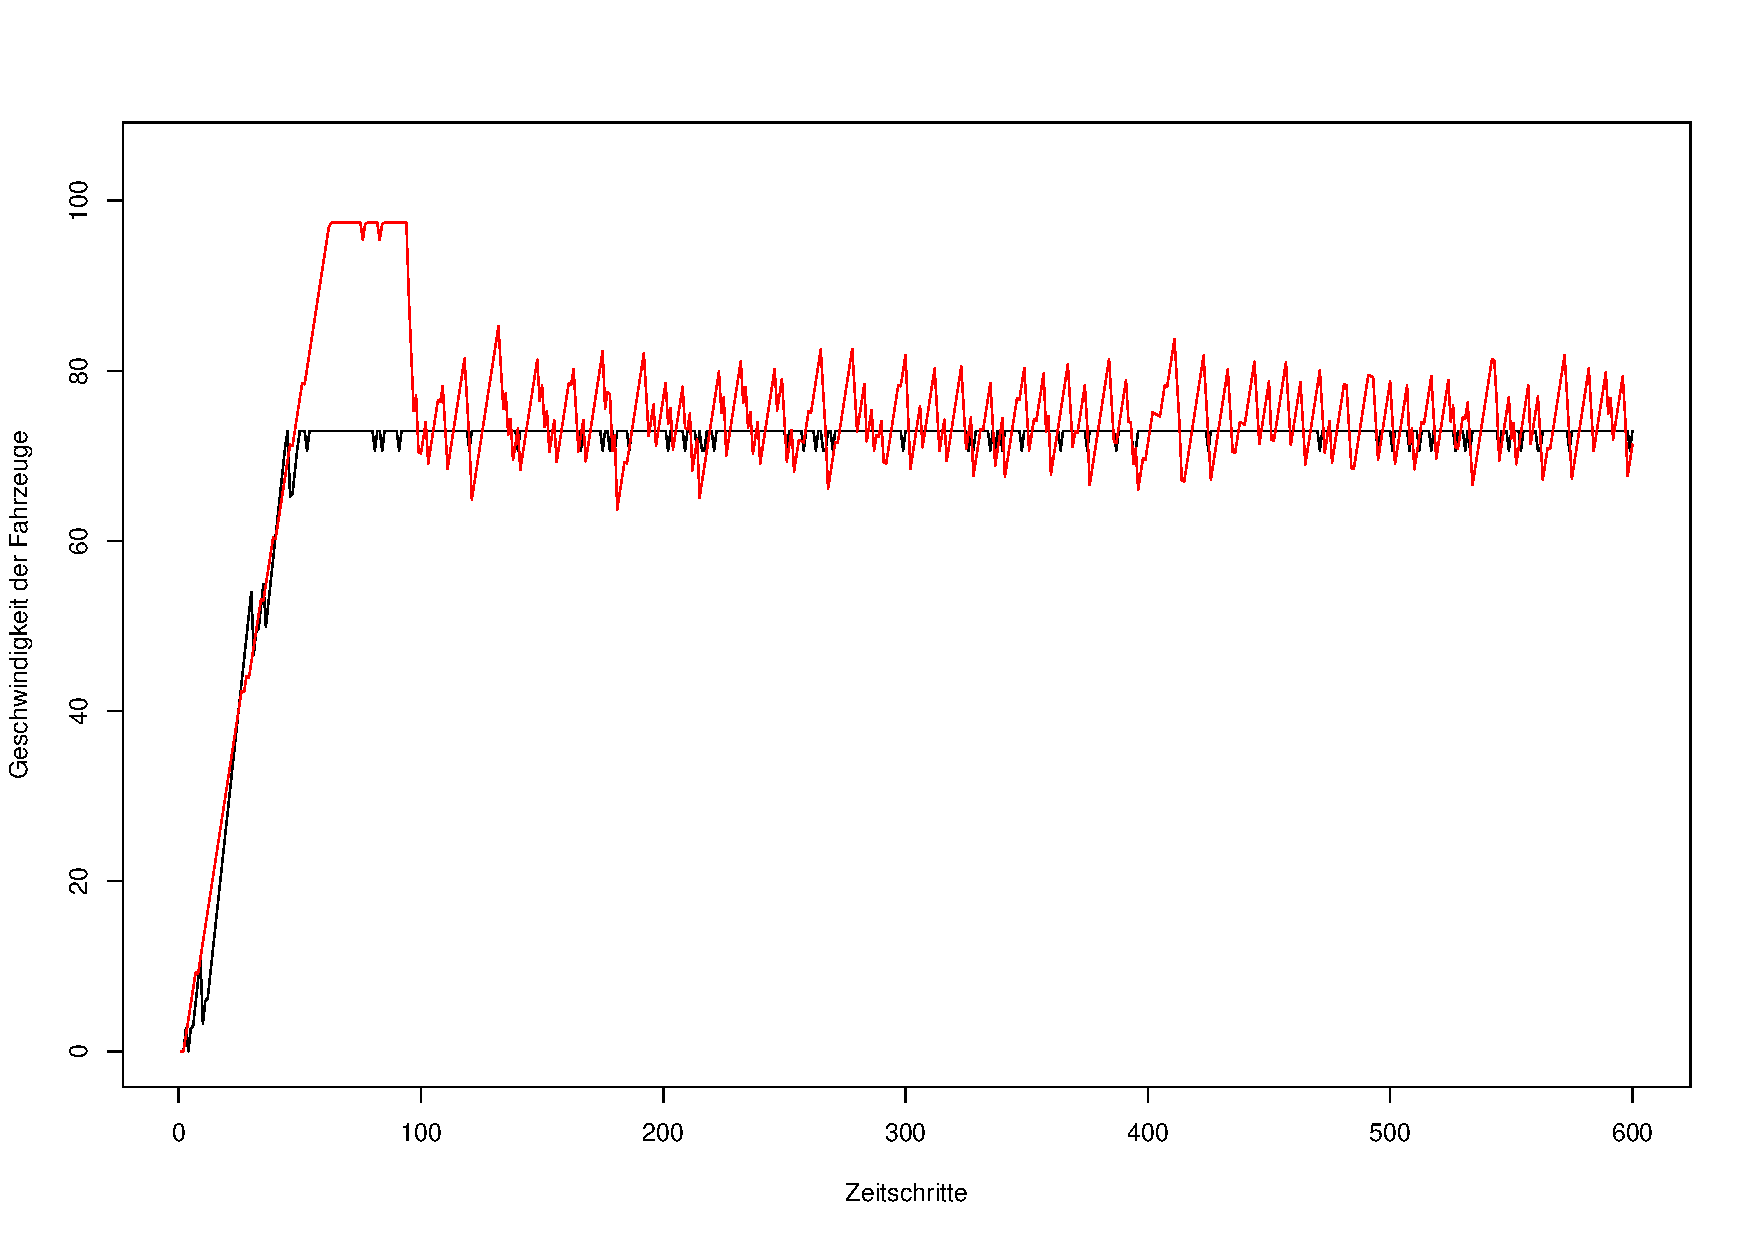
\includegraphics[width=0.3\textwidth]{speed_run15}\label{figure:run15}}\qquad 
   \subfigure[3. Durchlauf]{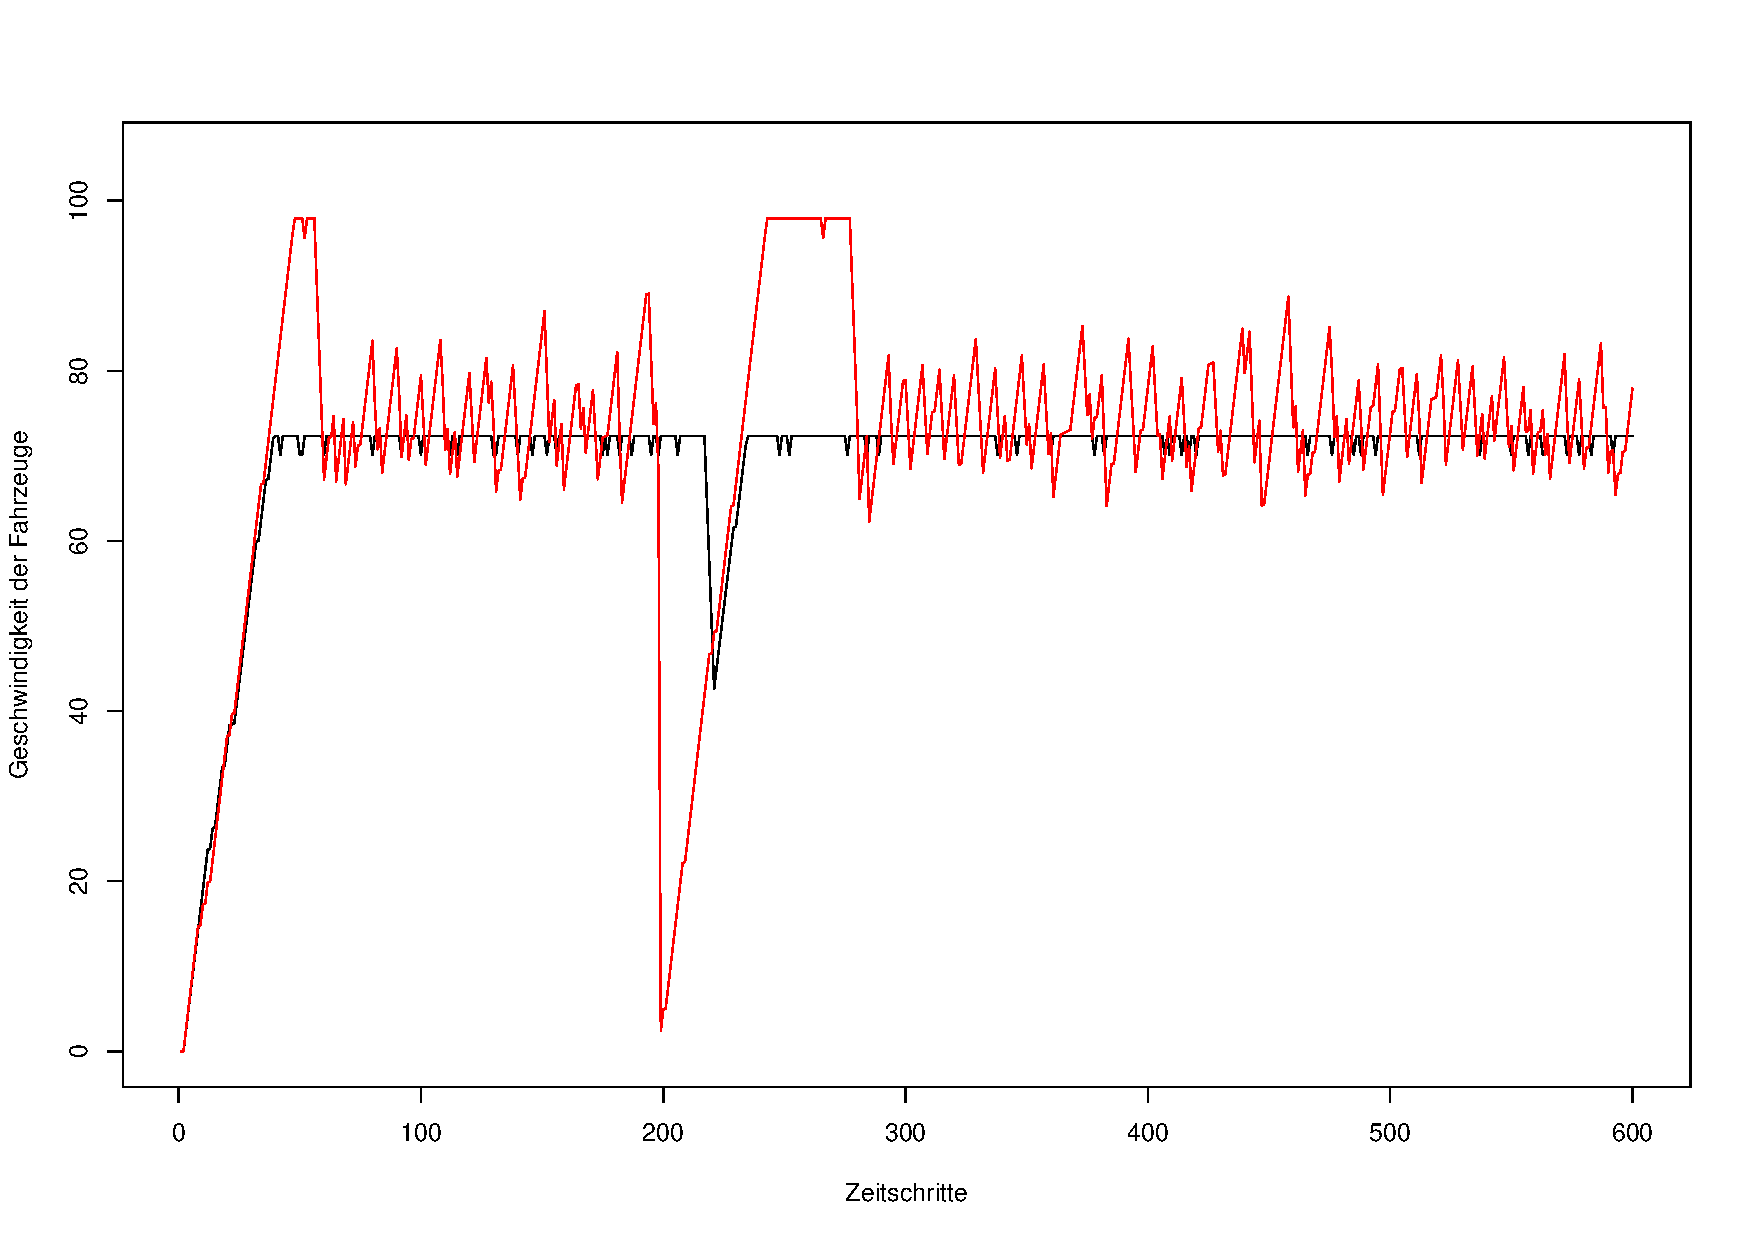
\includegraphics[width=0.3\textwidth]{speed_run16}\label{figure:run16}}
  \caption{Simulationen mit Zellgröße 5,0 m und Zeitschrittlänge 0,05 min} 
  \label{figure:run14-16}
\end{figure}

Die Diagramme in \cref{figure:run14-16} zeigen wiederholt, dass der Abstand, der für den Bremsvorgang zur Verfügung steht, mit einem recht langen Zeitraum zwischen den Zeitschritten, nicht ausreicht.

Allerdings ist im ersten und im dritten Durchlauf zu erkennen, dass das langsamere Fahrzeug, ohne dass es zu einer Kollision kommen muss, für das gerade beschleunigende Fahrzeug abbremsen konnte. 

\begin{figure}[hptb]
  \centering 
   \subfigure[1. Durchlauf]{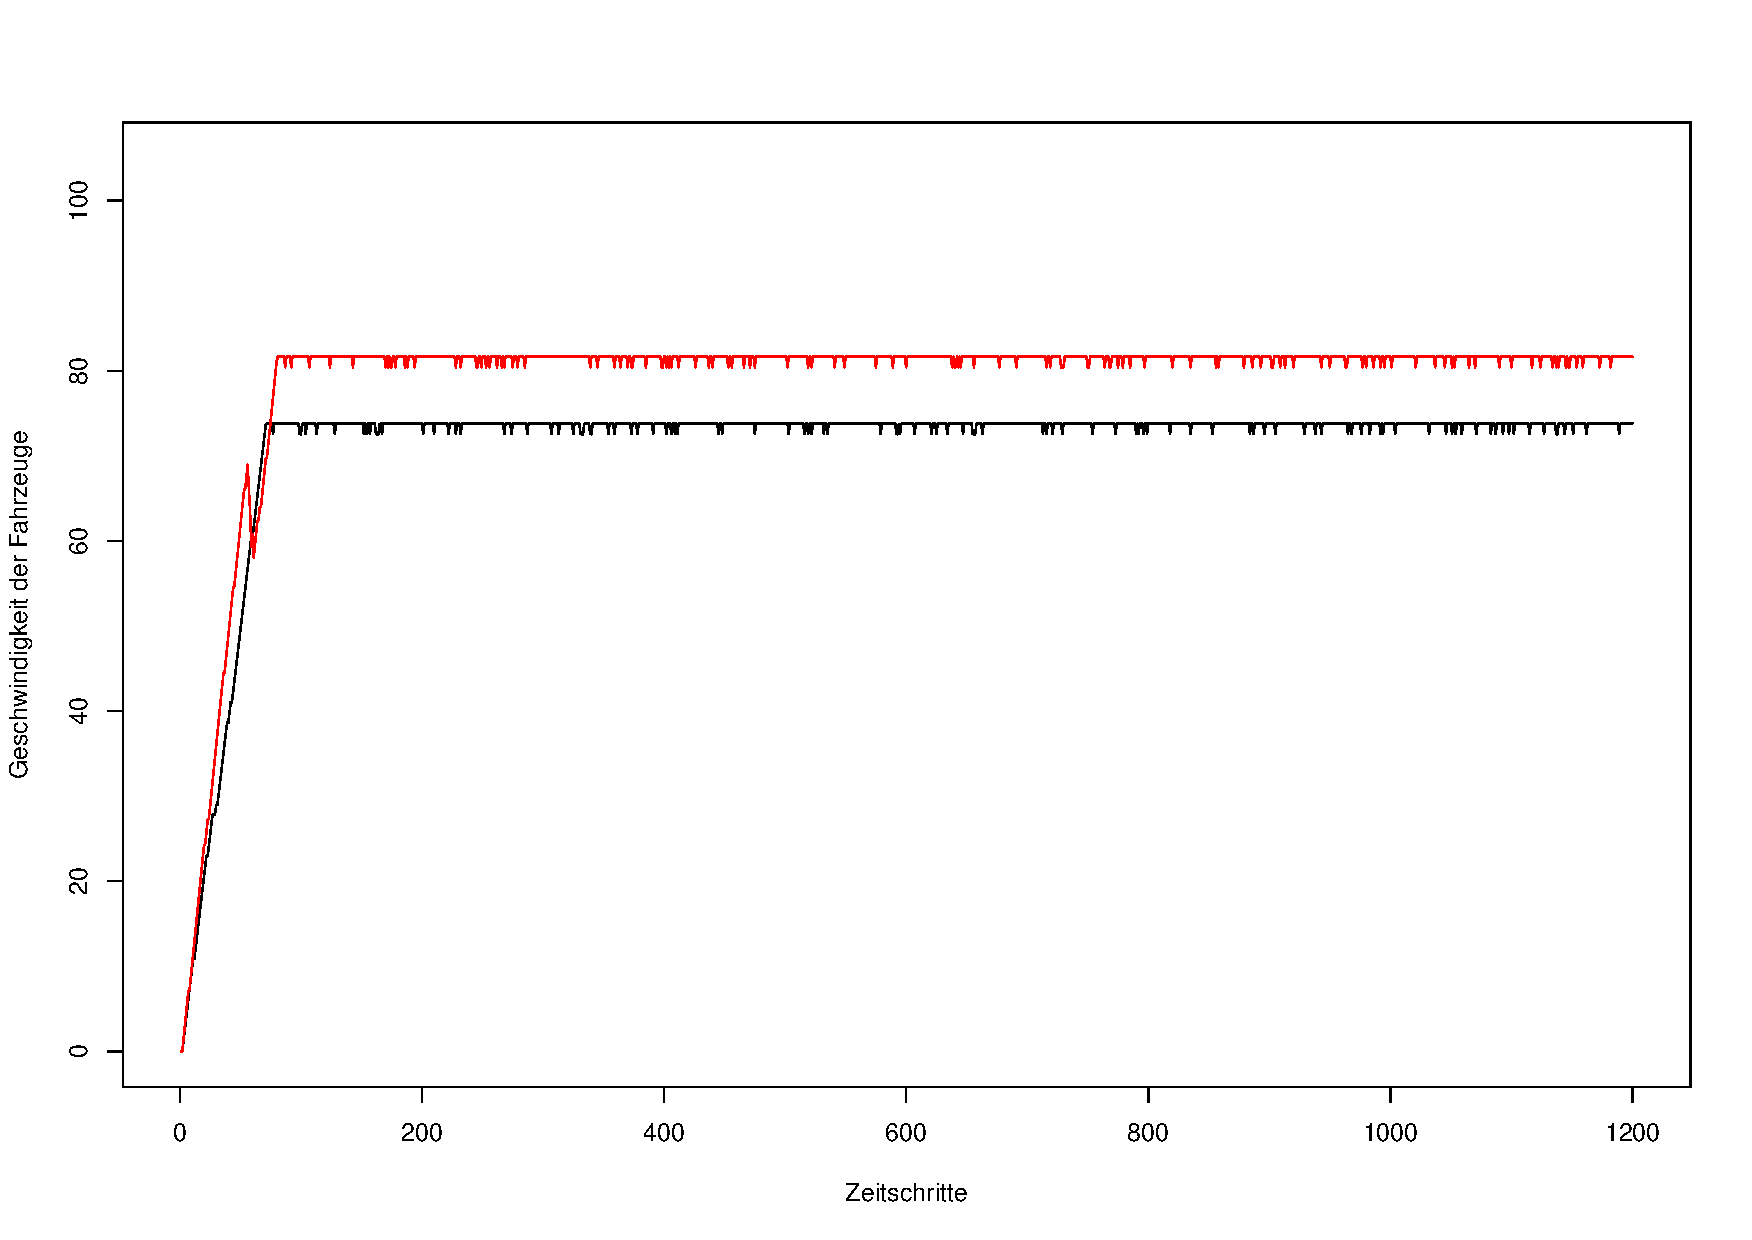
\includegraphics[width=0.3\textwidth]{speed_run17}\label{figure:run17}}\qquad 
   \subfigure[2. Durchlauf]{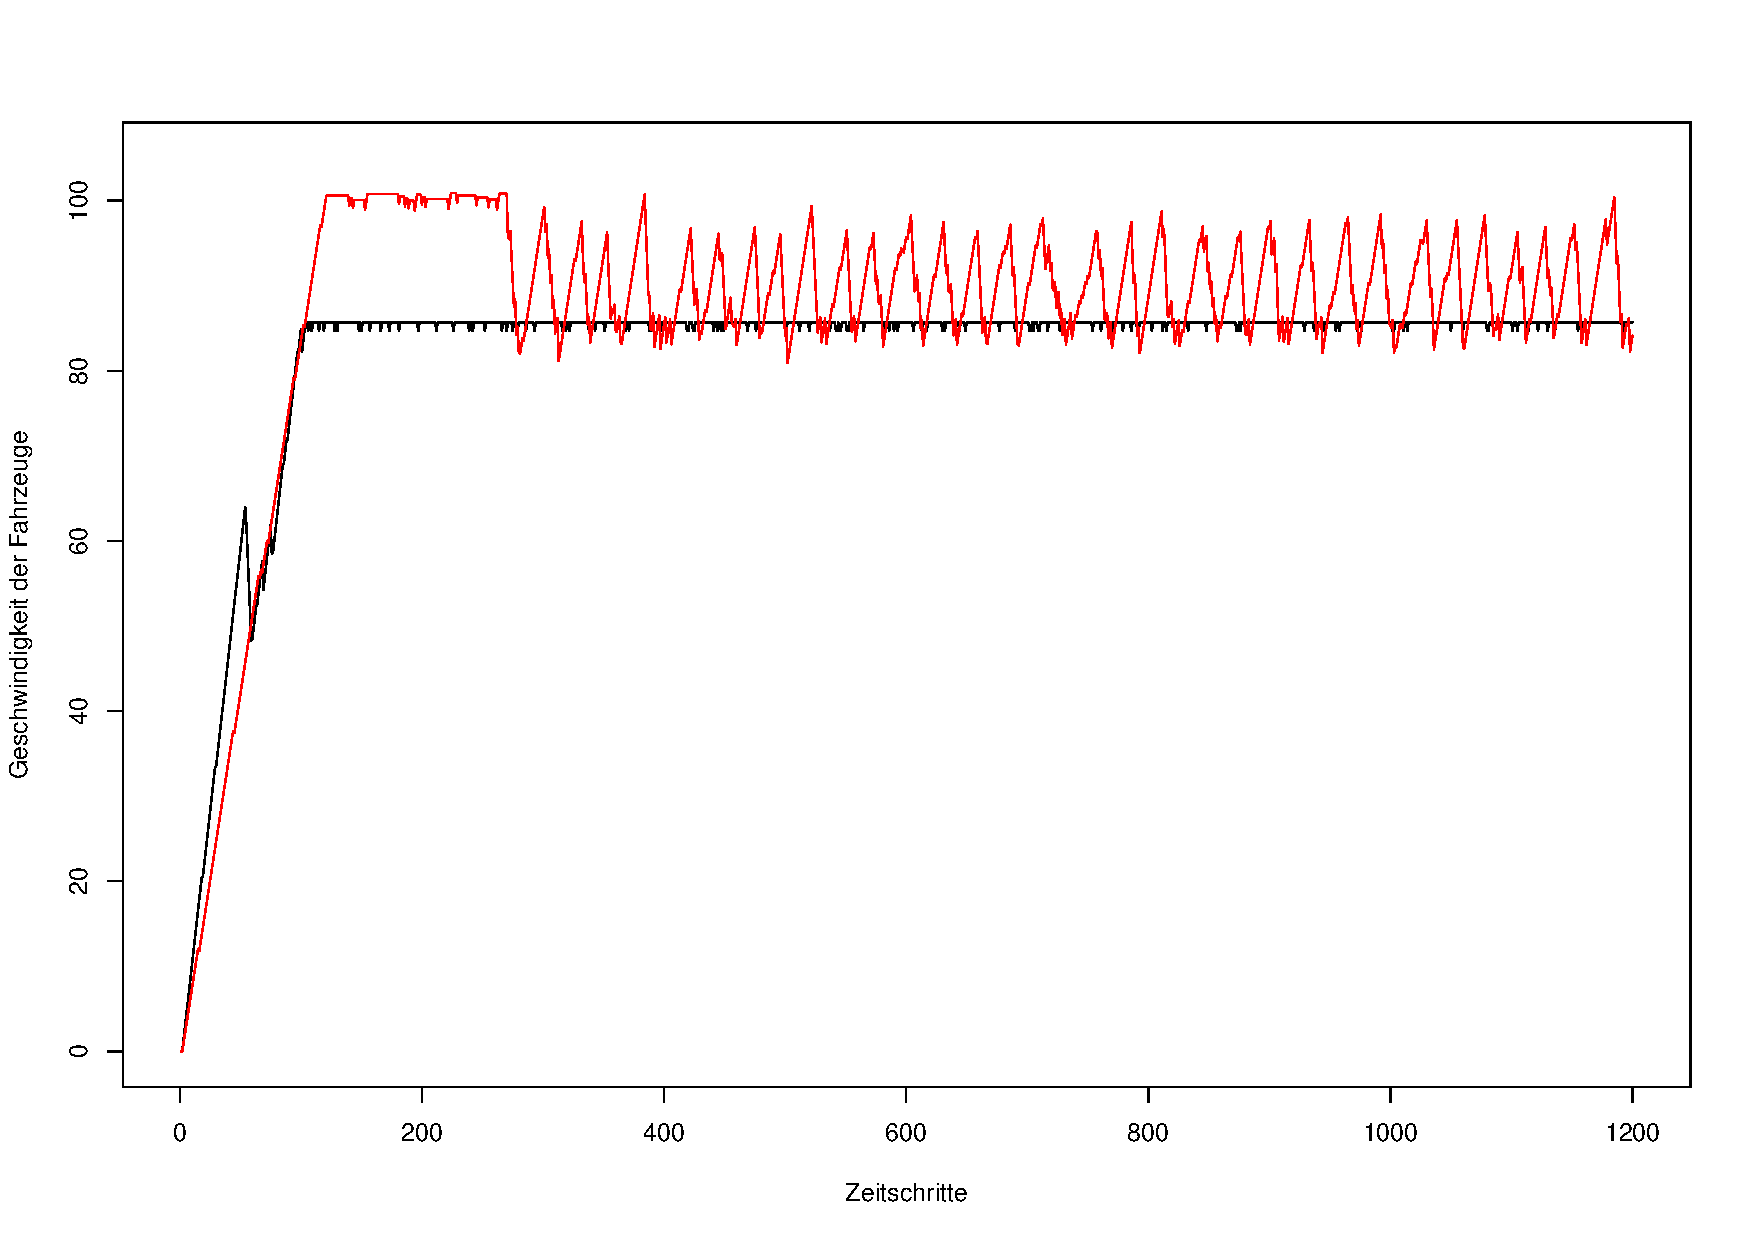
\includegraphics[width=0.3\textwidth]{speed_run18}\label{figure:run18}}\qquad 
   \subfigure[3. Durchlauf]{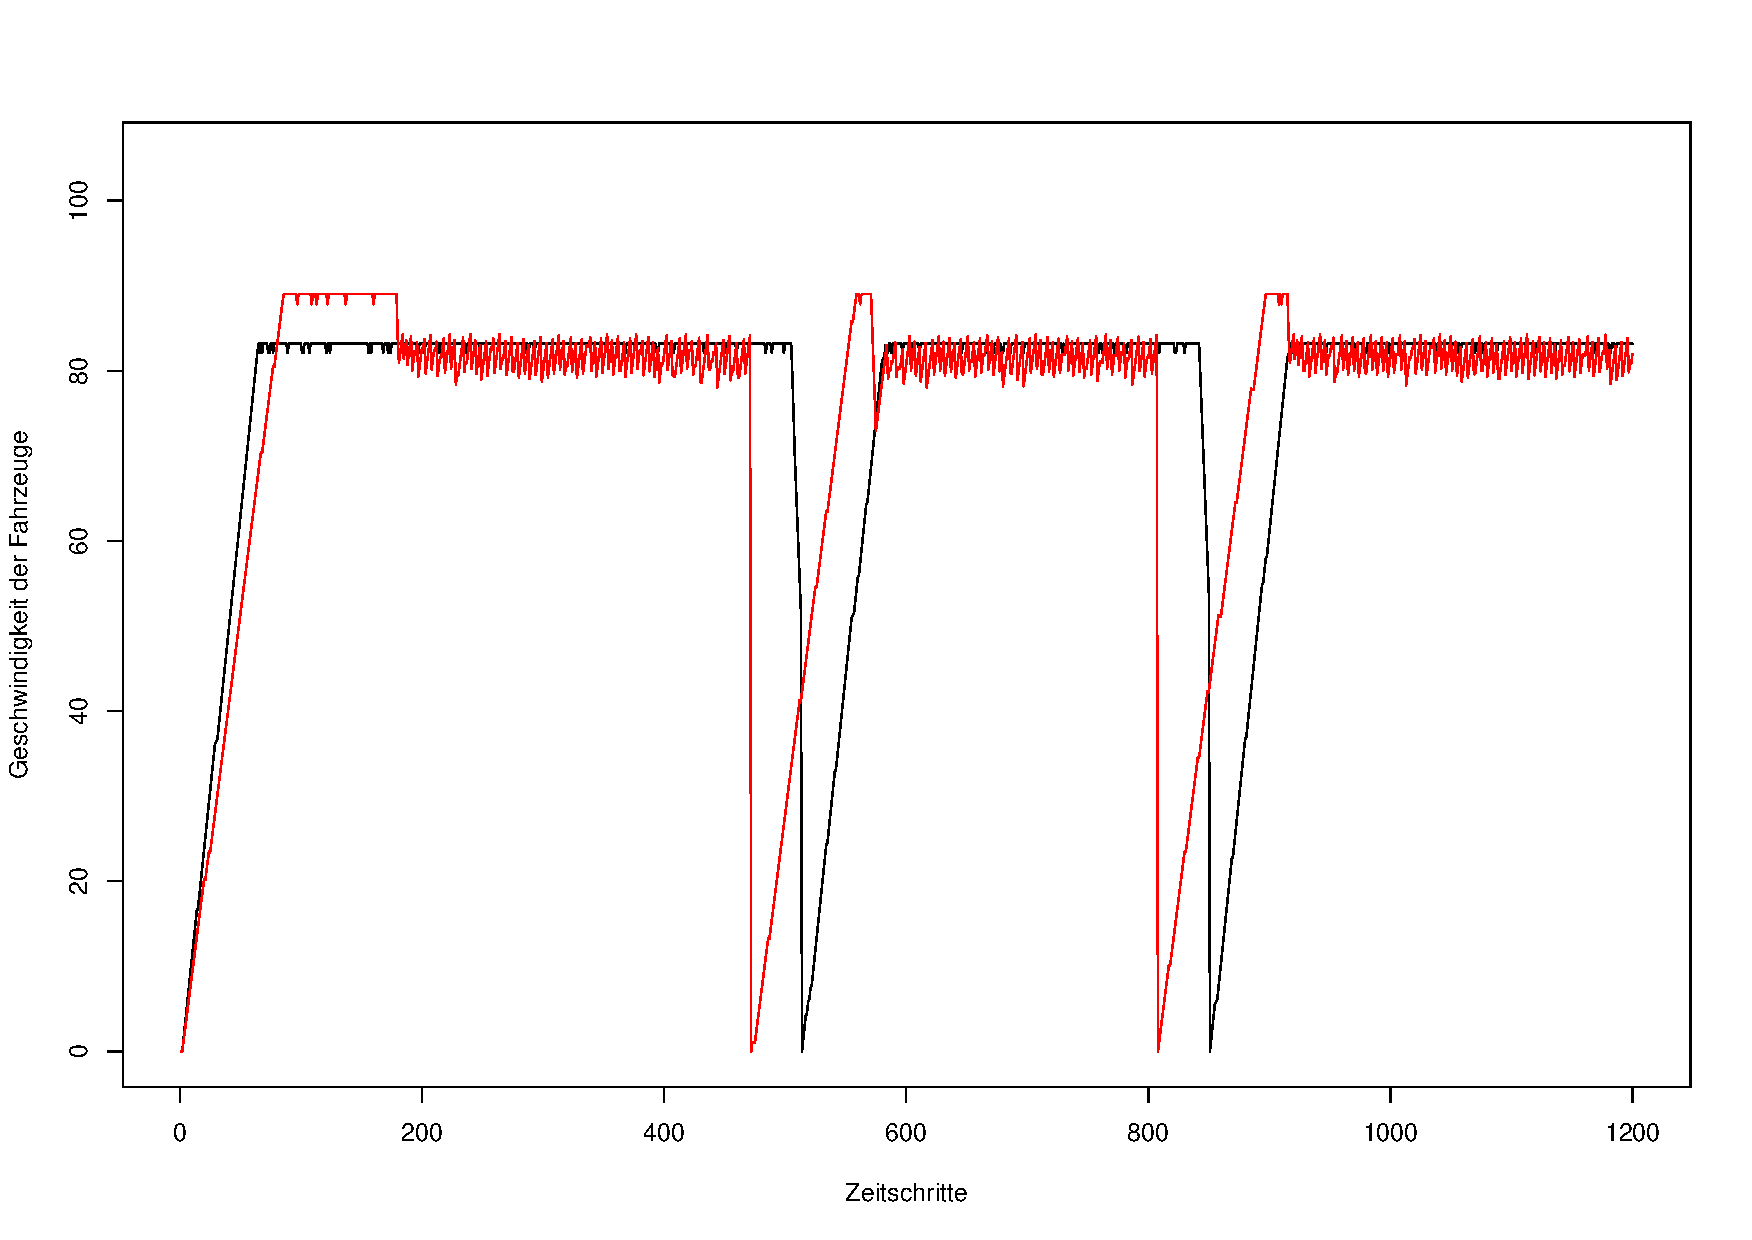
\includegraphics[width=0.3\textwidth]{speed_run19}\label{figure:run19}}
  \caption{Simulationen mit Zellgröße 5,0 m und Zeitschrittlänge 0,025 min} 
  \label{figure:run17-19}
\end{figure}

Die drei Durchläufe mit einer Zeitschrittlänge von 0,025 min ergaben ein uneinheitliches Bild.
In \cref{figure:run17} konnte das schnellere Fahrzeug wieder mit höherer Geschwindigkeit hinter dem langsameren herfahren, scheinbar ohne dass ein Raumgewinn passierte, der zu einer Verzögerung geführt hätte.
\\
Evtl. fuhr das schnellere Fahrzeug auch mit seiner max. möglichen Geschwindigkeit und der Geschwindigkeitsunterschied war so gering, das es in der Simulationszeit das langsamere Fahrzeug nicht erreichte.

Der Durchlauf im Diagramm in \cref{figure:run18} zeigt wieder das sägezahnähnliche Muster, wie es mit den größeren Zelldimensionen bereits der Fall war.

Unerwarteterweise kam es im dritten Durchlauf zu je zwei Kollisionen.
Besonders die jeweils auslösende Kollision des ursprünglich schnelleren Fahrzeuges war nicht zu erklären, da der Geschwindigkeitsunterschied in beiden Fällen minimal gewesen war.

Ein weiterer Durchlauf, siehe \cref{figure:run19a}, der einen vergleichbaren Ablauf hervorbrachte, bei dem aber die Ausgabe der Fahrzeugdaten im Kontrollfenster erfolgte, konnte das Verhalten aufklären.
Die Bedingung im Agentenplan waren so formuliert, dass das Folgefahrzeug dem vorausfahrenden folgen konnte, ohne dass ein \enquote{Sicherheitsabstand} gebildet wurde, wenn die Geschwindigkeit jenes Fahrzeuges nicht größer als die des vorausfahrenden Fahrzeuges war. 
\\
Somit genügte, gewisse Geschwindigkeiten vorrausgesetzt, eine kleine Beschleunigung, ggf. bei Zusammentreffen mit einem Trödelvorgang des langsameren Fahrzeugs, um im nachfolgenden Zeitschritt die für die Geschwindigkeit erforderliche Wegstrecke nicht mehr umsetzen zu können.

\begin{figure}[hptb]
  \centering 
   \subfigure[ursprüngliches Verhalten]{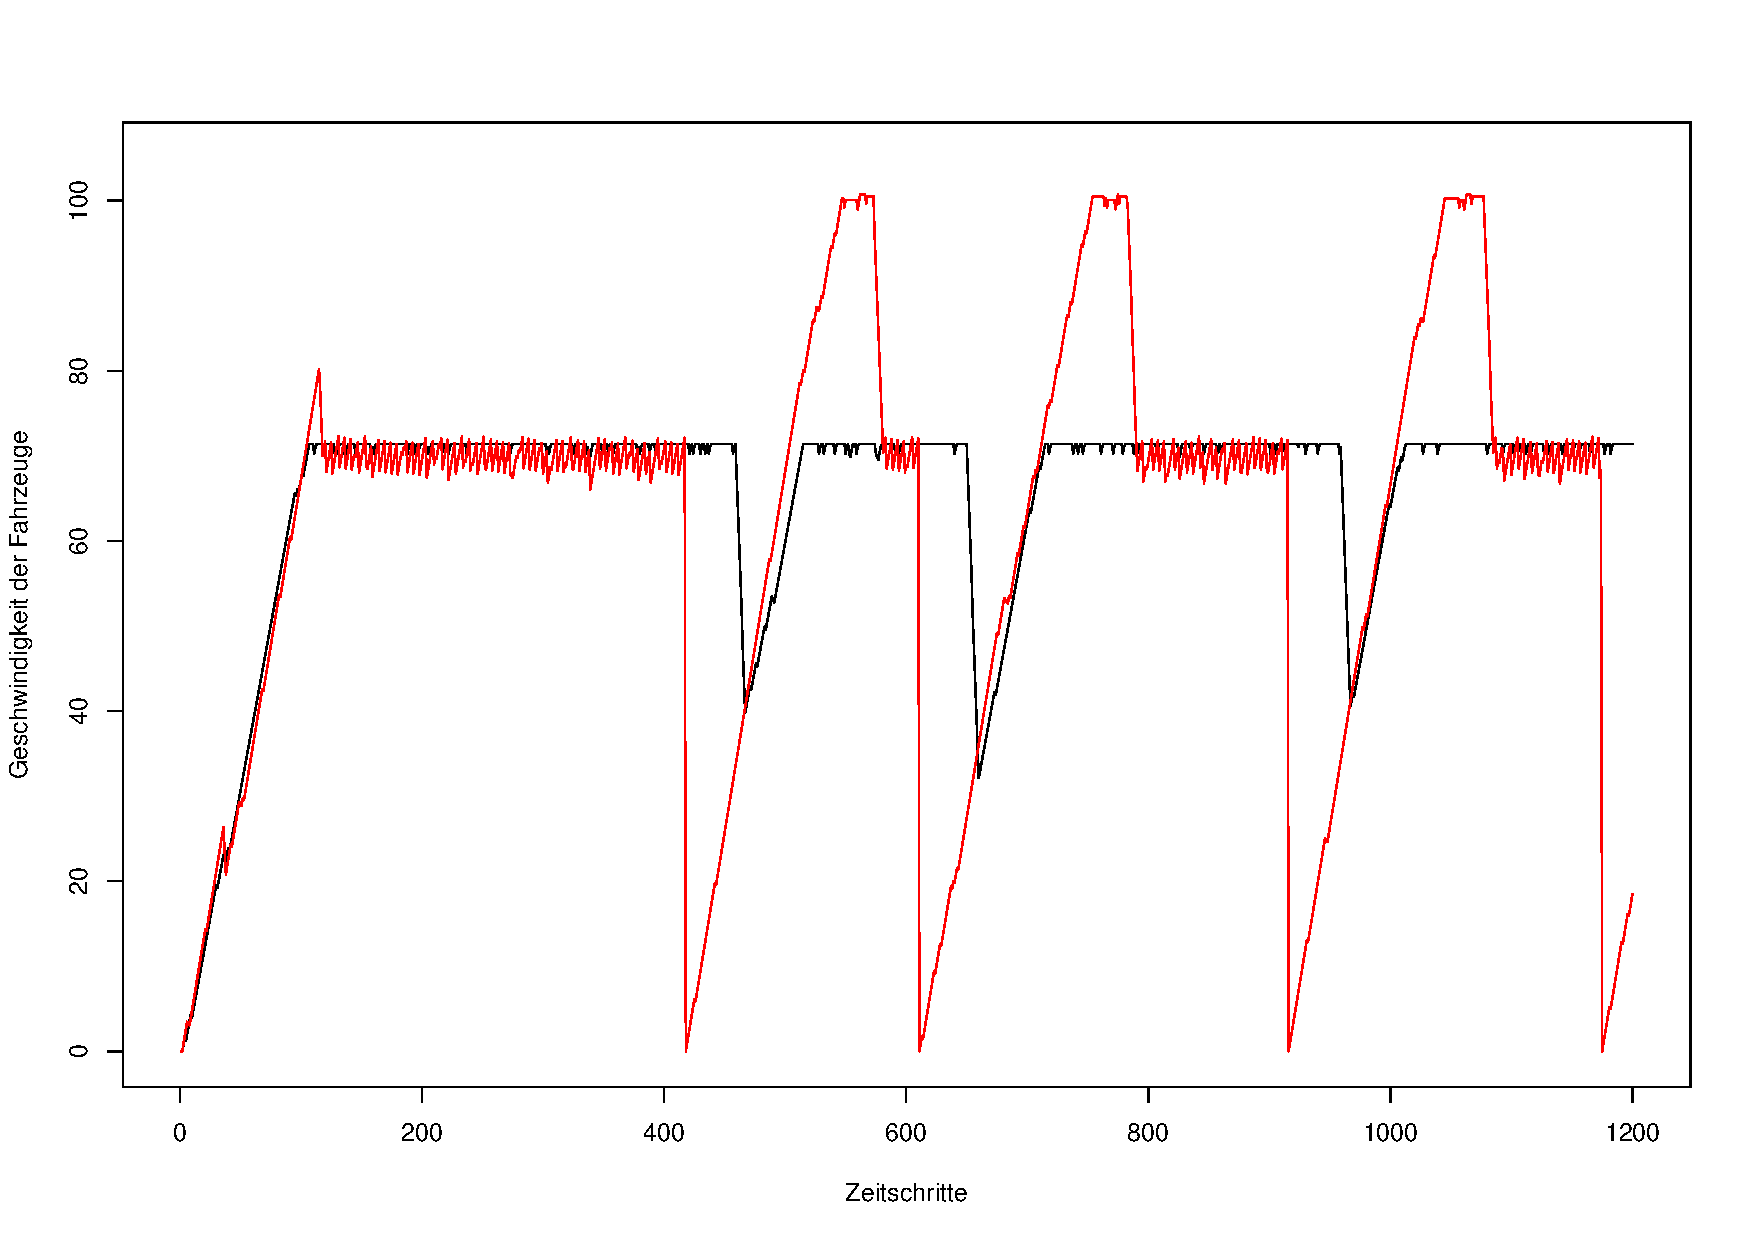
\includegraphics[width=0.3\textwidth]{speed_run19a}\label{figure:run19a}}\qquad 
   \subfigure[Modifikation 1]{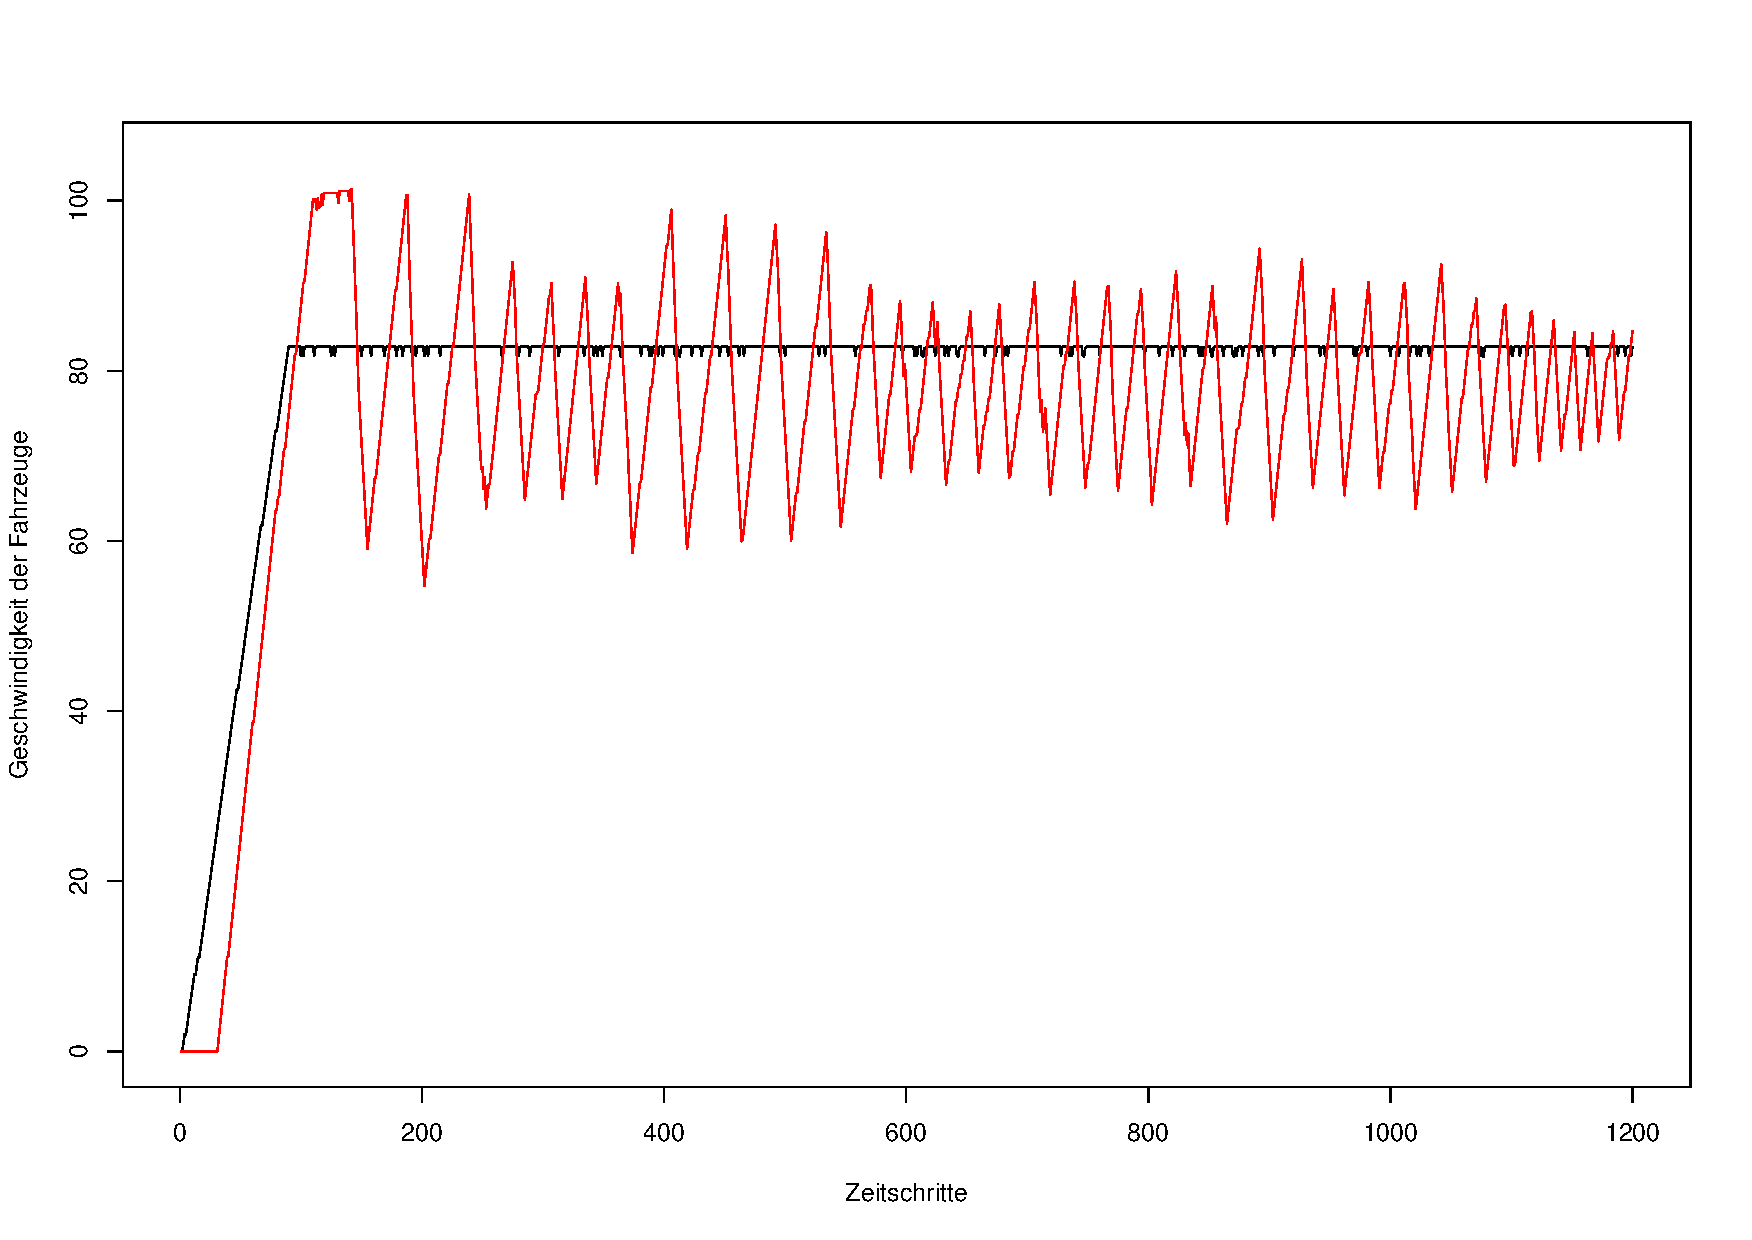
\includegraphics[width=0.3\textwidth]{speed_run19b}\label{figure:run19b}}\qquad 
   \subfigure[Modifikation 2]{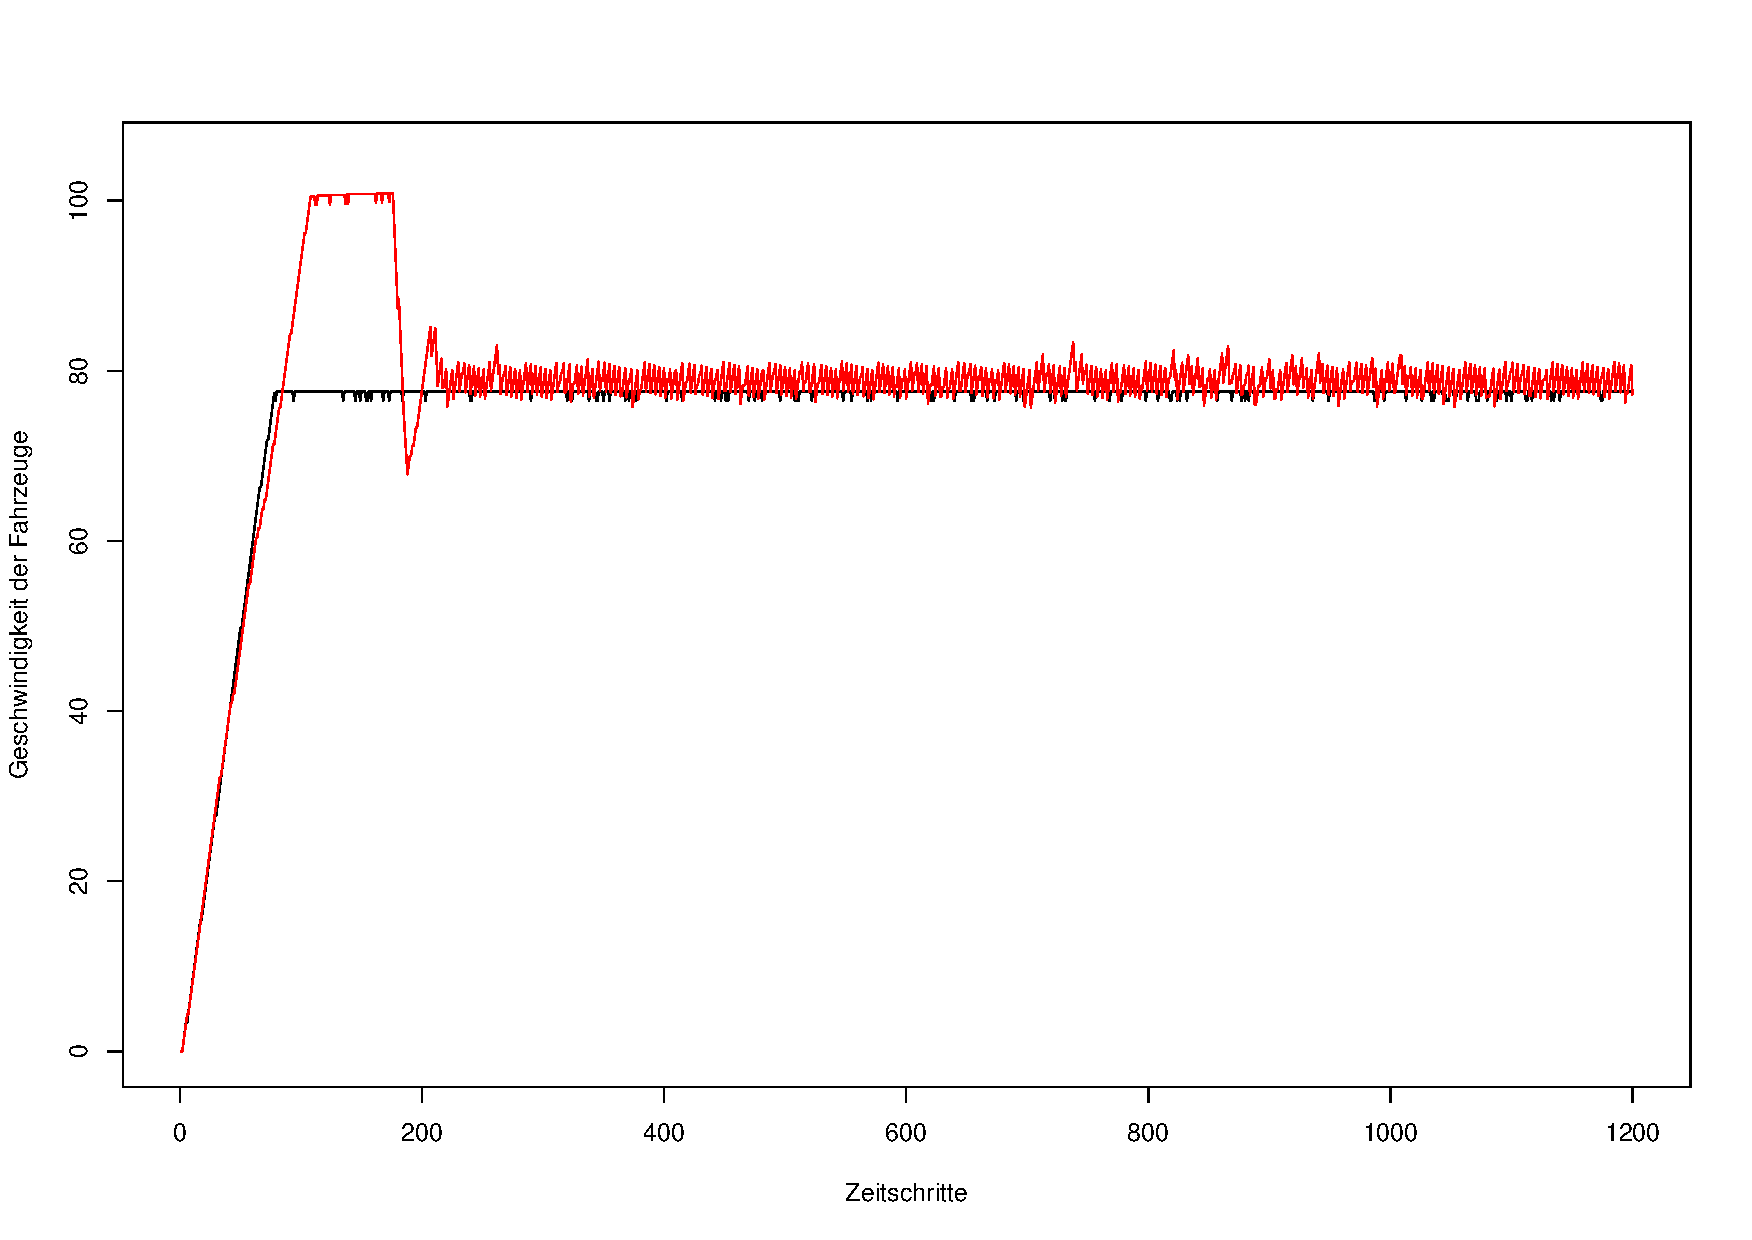
\includegraphics[width=0.3\textwidth]{speed_run19c}\label{figure:run19c}}
  \caption{Simulationen mit Veränderungen in den Agentenplänen} 
  \label{figure:run19a-c}
\end{figure}

Eine erste Modifikation führte wieder zurück zu einem Verhalten, siehe \cref{figure:run19b}, aufgrund dessen die Geschwindigkeitskomponente mit in die Verzögerungslogik eingefügt worden war. 
\\
Das nachfolgende Fahrzeug bremste so lange ab, bis der gewünschte Abstand erreicht war, um daraufhin mit einem \enquote{Zwischensprint} wieder auf das vorausfahrende Fahrzeug aufzuschließen.
Durch den Geschwindigkeitsüberschuss, der abgebaut werden muss, wurde der Abstand wieder extrem verlängert, dass der Kreislauf von vorn beginnt.
\\
In einigen Simulationsläufen musste die Geschwindigkeit derart massiv abgebaut werden, dass das Folgefahrzeug fast zum Stillstand kam.

Es musste ein Weg gefunden werden, die Geschwindigkeit eines Fahrzeuges in Zusammenhang mit der Entfernung vom vorausfahrenden Fahrzeug zu bringen.
\\
Verschiedene Ansätze, bei denen in den Bedingungen der Logik mit den vorliegenden Werten Berechnungen durchzuführen gewesen wären, wurden von der Simulationsplattform nicht unterstützt.
\\
Da aber den Agenten sowohl die eigene Geschwindigkeit als auch die Entfernung als numerische Werte bekannt sind, werden diese nun zu einander in Beziehung gesetzt.

Dies führt dazu, dass die Geschwindigkeit des betrachteten Fahrzeugs gleichzeitig der jeweilige Mindestabstand vom Vordermann sein muss. 
Hier wurde zu einem späteren Zeitpunkt noch der Faktor 1,5 eingefügt.
\\
Eine gleichwertige Bedingung wurde auch für die Simulation der Beschleunigung übernommen.
Der reine Geschwindigkeitsvergleich wurde entfernt.


\paragraph*{Zellgröße 2,5 m}
\hfill \\
Aufgrund der Veränderung in den Agentenplänen wurde die erneut verringerte Zellgröße ebenfalls mit den beiden noch verbliebenen Zeitschrittwerten simuliert.

\begin{figure}[hptb]
  \centering 
   \subfigure[1. Durchlauf]{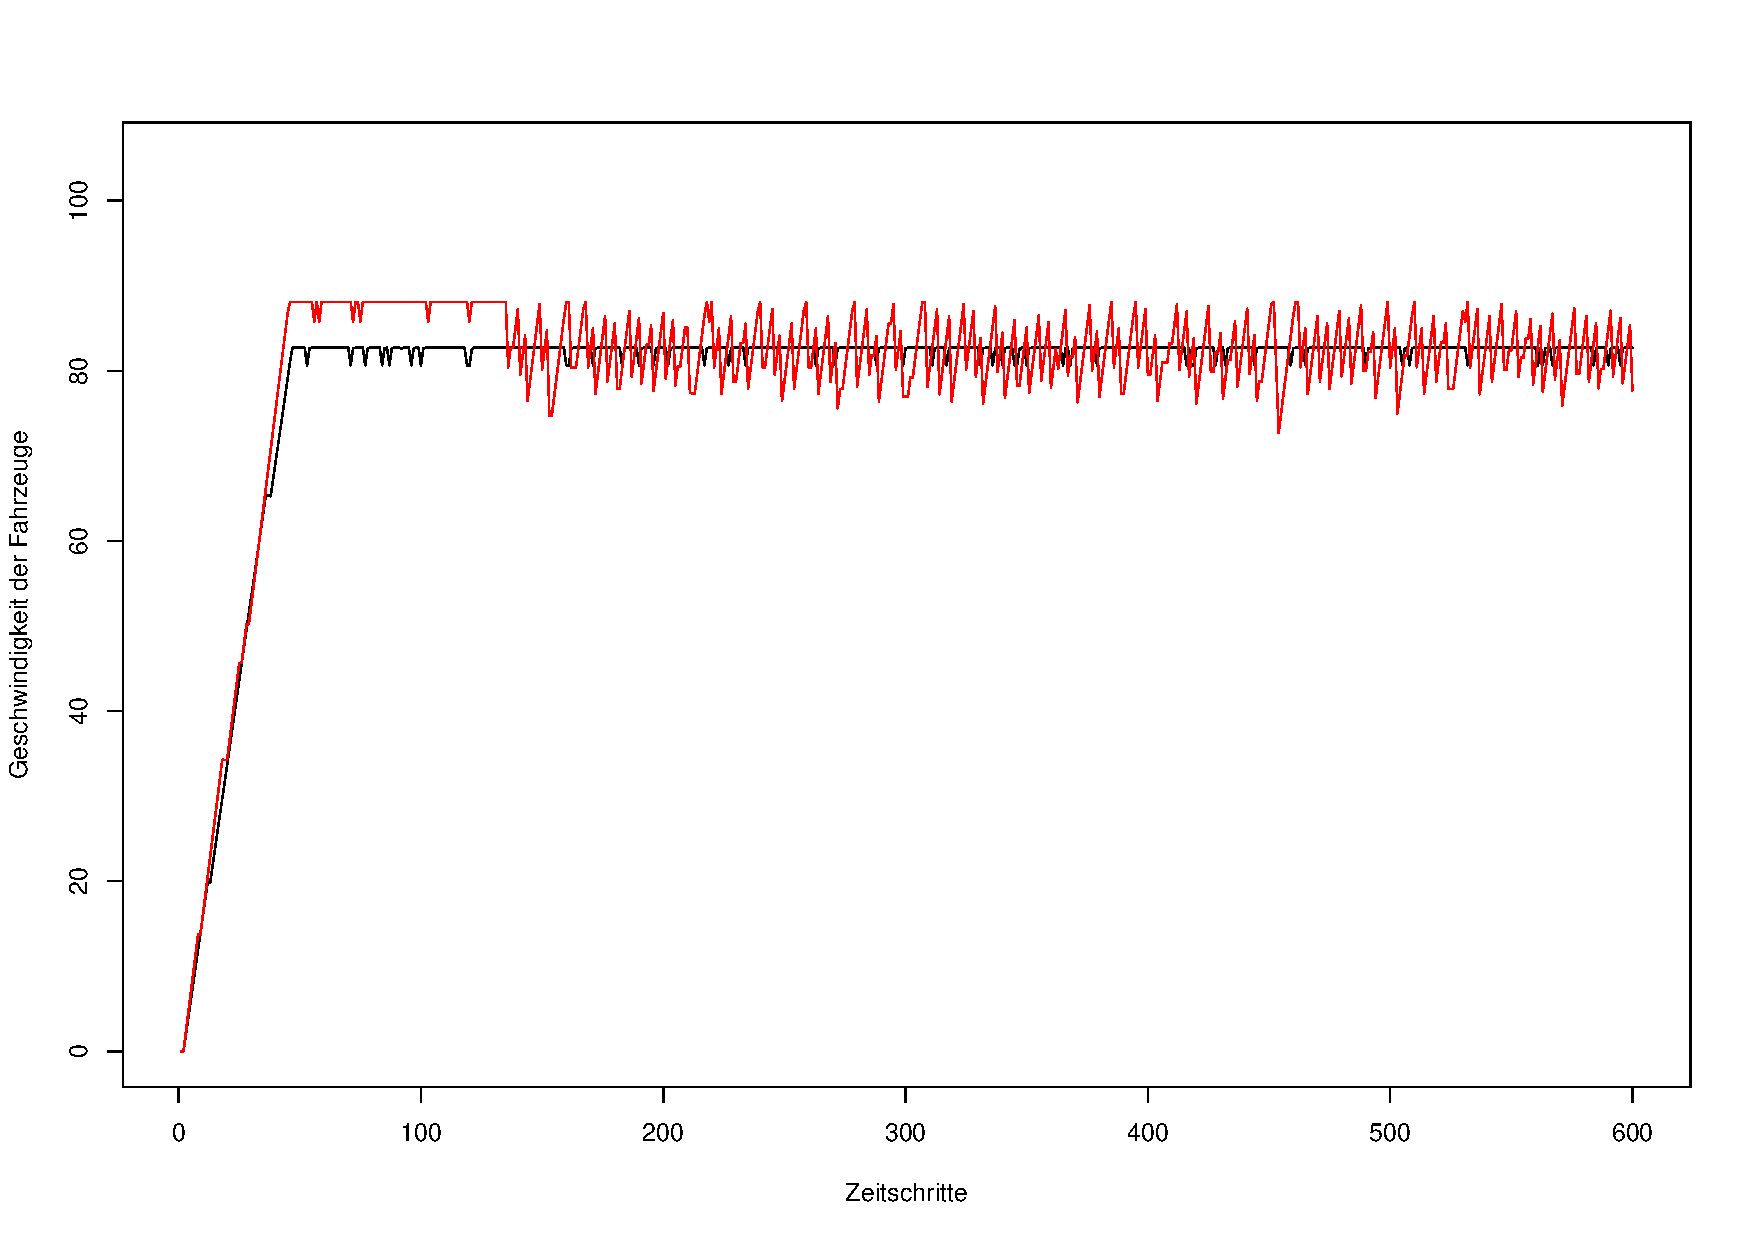
\includegraphics[width=0.3\textwidth]{speed_run24}\label{figure:run24}}\qquad 
   \subfigure[2. Durchlauf]{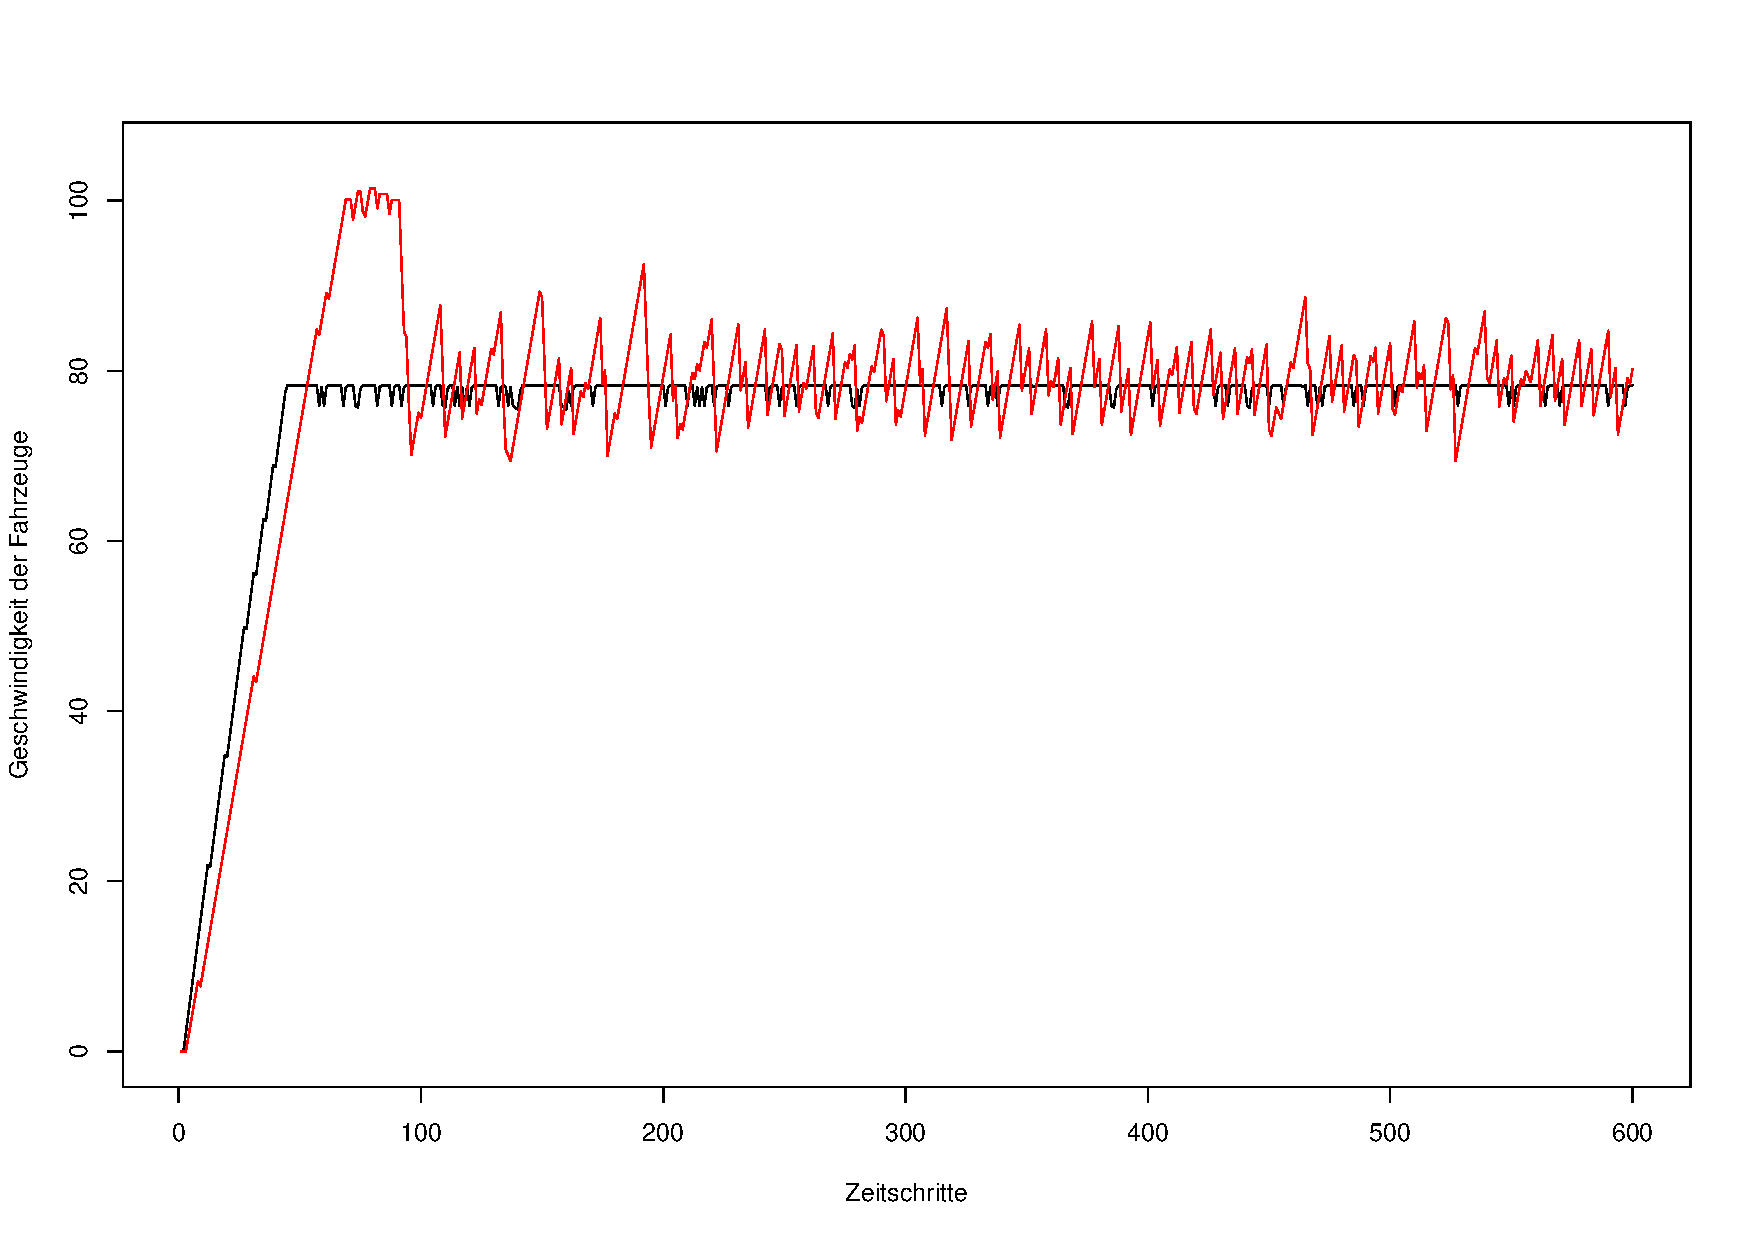
\includegraphics[width=0.3\textwidth]{speed_run25}\label{figure:run25}}\qquad 
   \subfigure[3. Durchlauf]{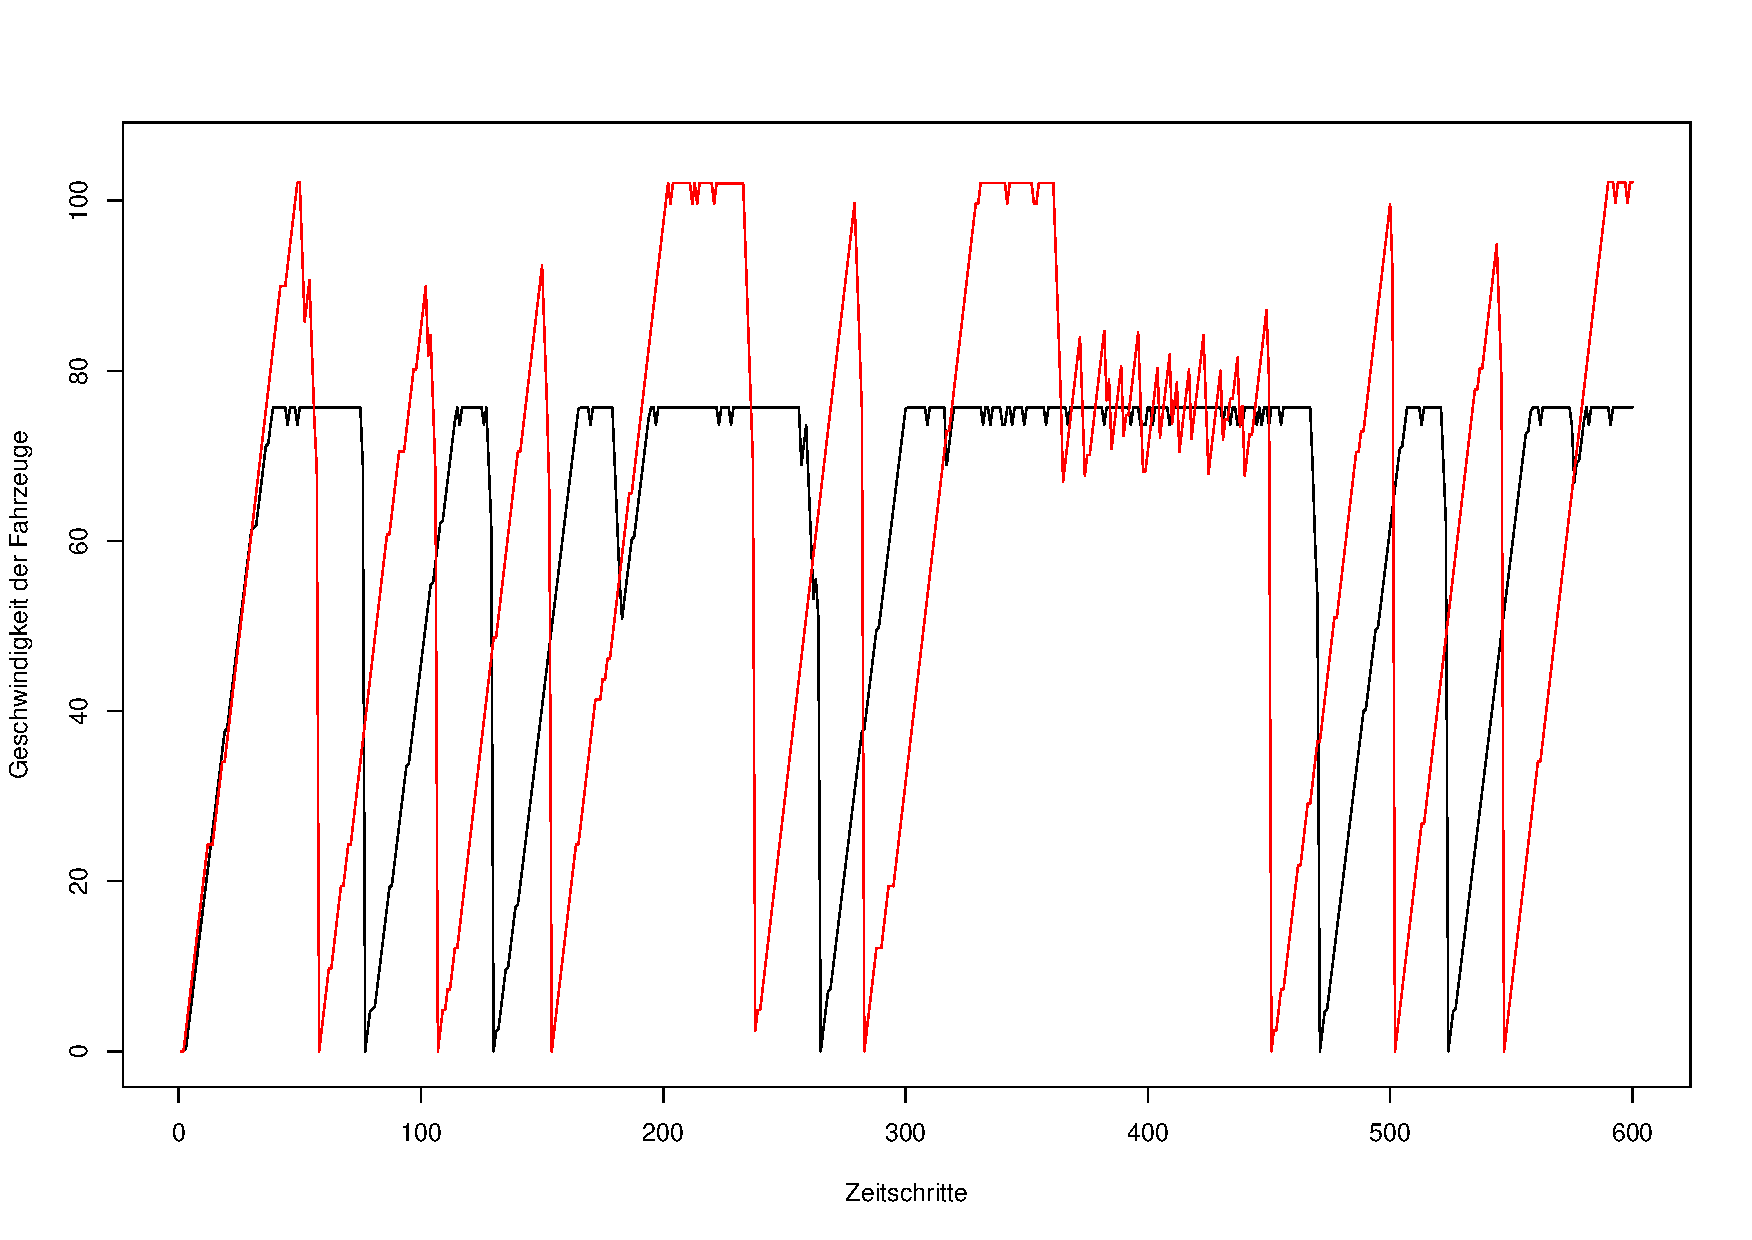
\includegraphics[width=0.3\textwidth]{speed_run26}\label{figure:run26}}
  \caption{Simulationen mit Zellgröße 2,5 m und Zeitschrittlänge 0,05 min} 
  \label{figure:run24-26}
\end{figure}

Die ersten beiden Simulationen mit 2,5 m/0,05 min zeigten ein Bild, welches nach den Veränderungen zu erwarten war.
In der dritten Durchführung traten allerdings wieder Kollisionsereignisse auf.

\begin{figure}[hptb]
  \centering 
   \subfigure[1. Durchlauf]{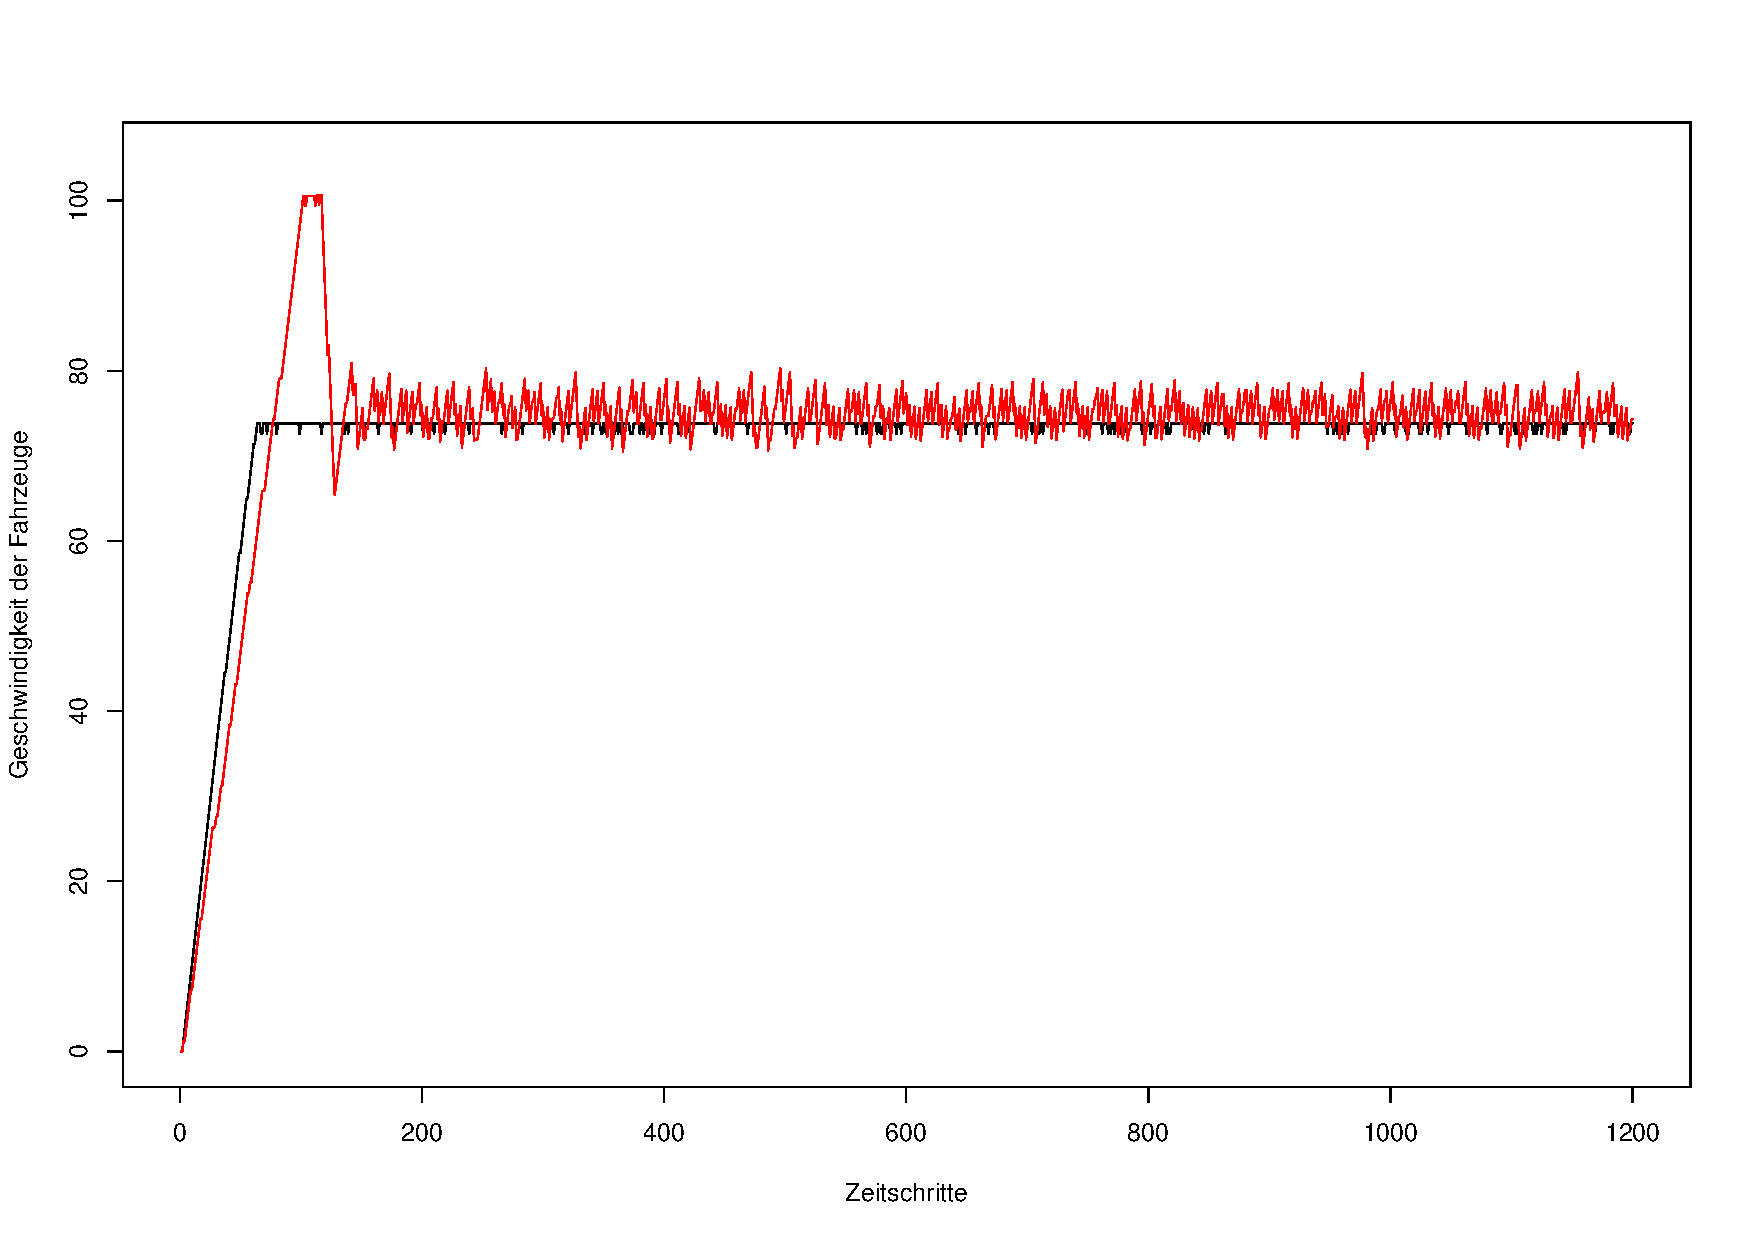
\includegraphics[width=0.3\textwidth]{speed_run27}\label{figure:run27}}\qquad 
   \subfigure[2. Durchlauf]{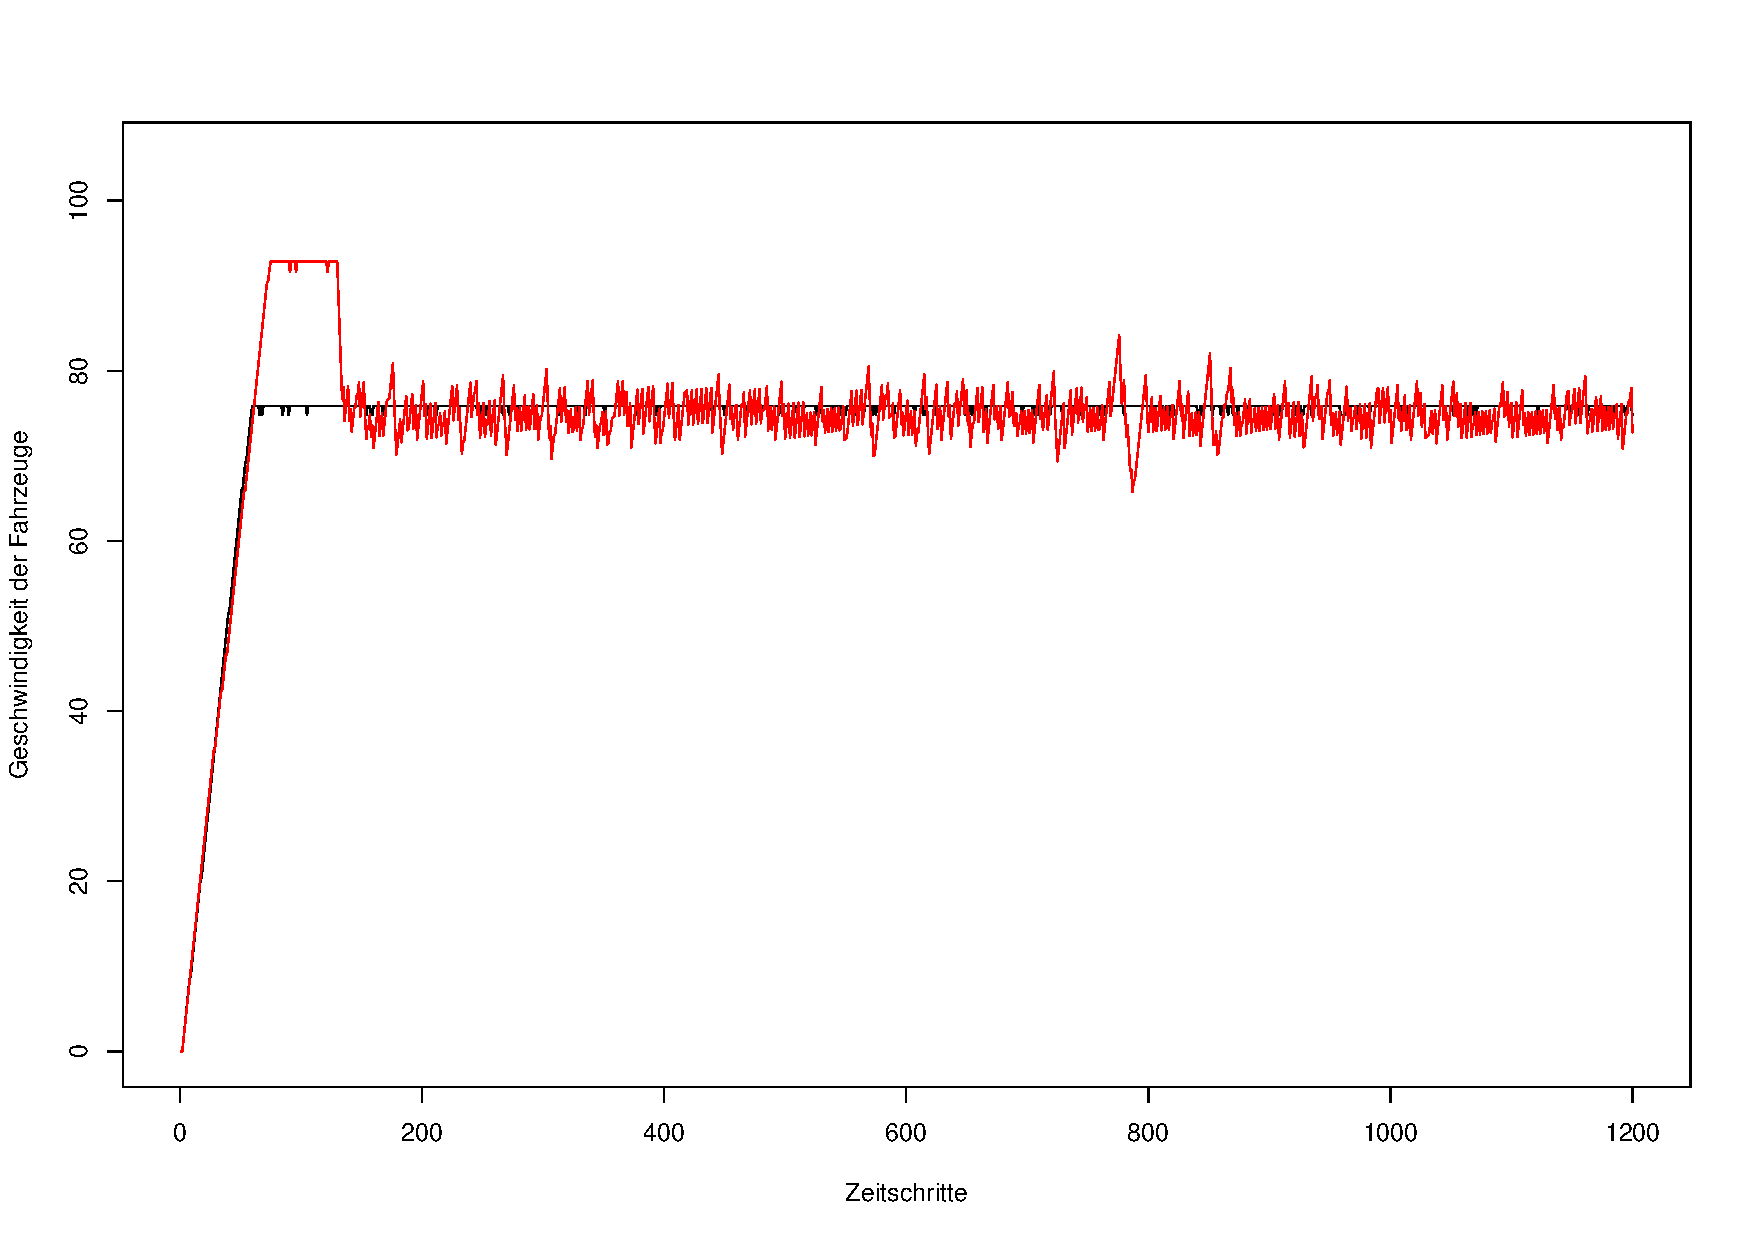
\includegraphics[width=0.3\textwidth]{speed_run28}\label{figure:run28}}\qquad 
   \subfigure[3. Durchlauf]{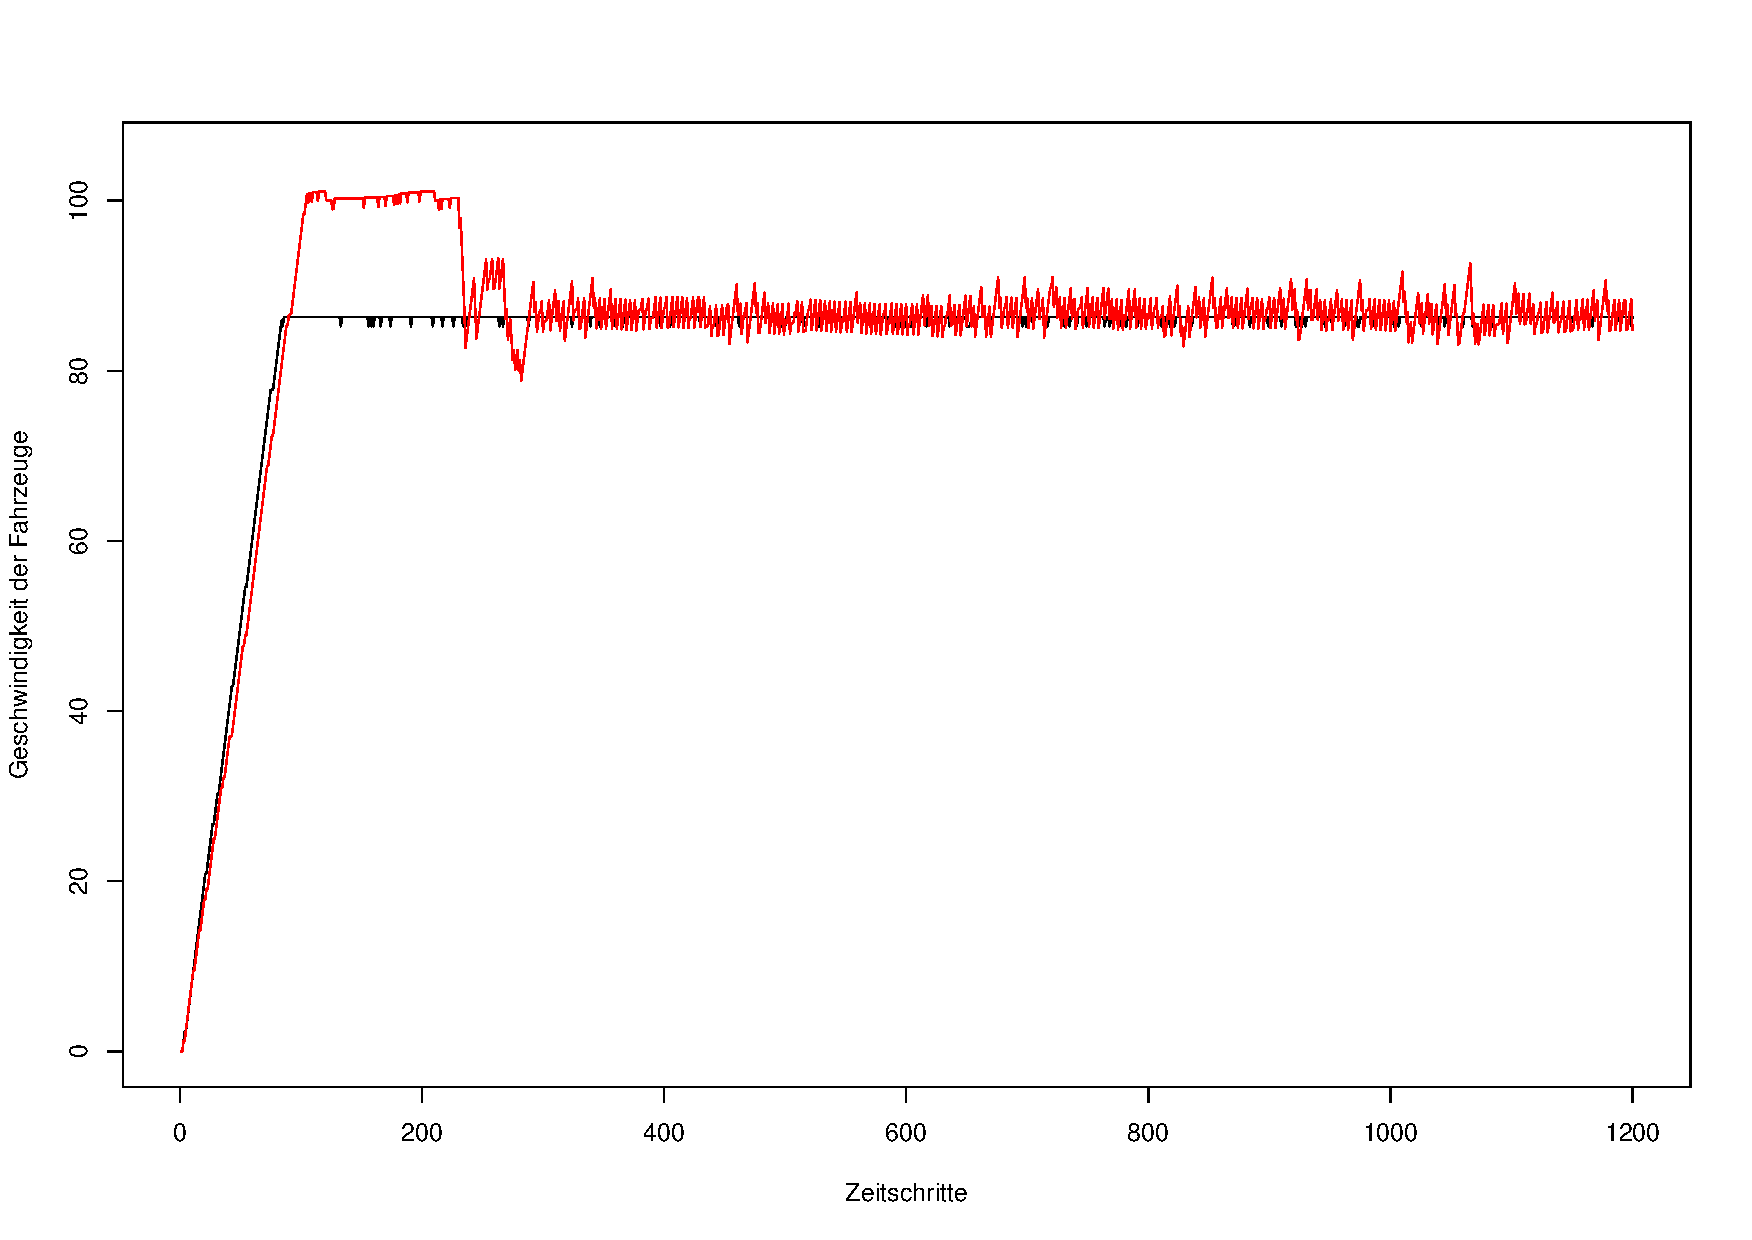
\includegraphics[width=0.3\textwidth]{speed_run29}\label{figure:run29}}
  \caption{Simulationen mit Zellgröße 2,5 m und Zeitschrittlänge 0,025 min} 
  \label{figure:run27-29}
\end{figure}

Die Simulationen der 2,5 m/0,025 min-Variante (\cref{figure:run27-29}) zeigten ein, nach den bisherigen Erfahrungen, erwartetes und gewünschtes Verhalten.
Das schnelle Fahrzeug konnte ohne Kollision hinter dem langsamen Fahrzeug abbremsen und sich dessen Geschwindigkeit anpassen.
\\
Es wurden insgesamt zehn weitere Durchgänge mit diesem Setup durchgeführt. 
Dabei wurde zweimal je eine Kollision beobachtet, die aber immer im Bereich der Beschleunigungsphase am Anfang der Simulation stattfand. 


\paragraph*{\texorpdfstring{Zellgröße $ < $ 2,5 m}%
                              {Zellgröße kleiner als 2,5 m}}
\hfill \\
Bei vorhergehenden Testläufen außerhalb dieser Reihe wurde festgestellt, dass es bei einer Zellgröße von weniger als 2,5 Meter zu Inkonsistenzen in den Beliefbases der Agenten kommt.
Entscheidungen müssten dann aufgrund unterschiedlicher Voraussetzungen getroffen werden.
Aus diesem Grund wurde auf den Einsatz von kleineren Zellgrößen verzichtet.






\subsection{Testläufe des Einspurszenarios}
\label{sec:test-singlelane}

Die Testläufe für den Einspurfall sollten mit den folgenden Einstellungen erfolgen:
\begin{itemize}
	\itemsep0em
	\item Simulationsdauer: 2 h
	\item Anzahl Fahrzeuge: variabel, siehe \cref{sec:fahrzeuganzahl}
	\item Anzahl Fahrspuren: 1
	\item Streckenlänge: 7,5 km 
	\item Zellgröße: 2,5 m
	\item Zeitschrittlänge: 0,025 min (1,5 sek)
	\item Intervalle Beschleunigung/Verzögerung/Geschwindigkeit: $ [3,5; 7] $/$ [8; 10] $/$ [80; 130] $
	\item max. Geschwindigkeit: 100 km/h
	\item Verhalten bei Kollisionsereignis: abbremsen (kein Totalstop)
\end{itemize}


\paragraph*{Anpassung der Trödelwahrscheinlichkeit $p_{linger}$}
\label{sec:adjust-linger}
\hfill \\
Da es sich bei den Statistikwerten in \cref{sec:fahrzeuganzahl} um Tagesdurchschnitte handelt, darf angenommen werden, dass die daraus berechnete Verkehrsdichte für das Teilstück der A7 zwar eine hohe, aber noch zu bewältigende Verkehrsmenge ist.
In der Simulation sollte es also möglich sein, fließenden Verkehr zu generieren.

Der zuvor präferierte Wahrscheinlichkeitswert von 0,3 führte mit 34 Fahrzeugen allerdings mehrfach zu Stockungen und damit nicht zu einem ordentlichen Verkehrsfluss.
Aus diesem Grund wurden mit einer auf eine Stunde verkürzten Simulationsdauer kleinere Werte (erst 0,1-, dann 0,025-Schritte) und Veränderungen am Szenario getestet.

Die folgenden Beobachtungen wurden dabei getätigt:
\begin{enumerate}
	\itemsep0em
	\item bei Beseitigung der Geschwindigkeitsunterschiede (Anpassung des Geschwindigkeitsintervalls) waren Simulationsläufe mit dem angedachten $p_{linger}$-Wert möglich
	\item bei Deaktivierung des \texttt{linger}-Planes (unter Beibehaltung o.g. des Geschwindigkeitsintervalles) kam es teilweise zu starken Abbremsvorgängen
	\item erst bei einem $p_{linger}$-Wert zwischen 0,125 und 0,1 oder darunter konnte fließender Verkehr simuliert werden
\end{enumerate}

\subparagraph*{zu 2.} Durch die Inhomogenität der für die Fahrzeuge möglichen Geschwindigkeiten existiert immer (mind.) ein langsamstes Fahrzeug, auf das aufgelaufen wird.
Die Bremsreaktionen der Agenten in der Simulation scheinen zu einem vergleichbaren Verkehrsbild zu führen.

\subparagraph*{zu 3.} Aufgrund dieser Feststellung werden die Testläufe mit einer Trödelwahrscheinlichkeit von 0,125 durchgeführt.



\subsubsection{Verkehrsmenge A7: 34 Fahrzeuge}
\label{sec:szenario-a7}

Mit dem o.g. Wert gelangen mehrere Durchläufe, bei denen fließender Verkehr mit Fluktuation der Geschwindigkeiten der Fahrzeuge simuliert werden konnte.

\sa{own: change images}
\begin{figure}[hptb]
  \centering 
   \subfigure[Fahrzeugpositionen]{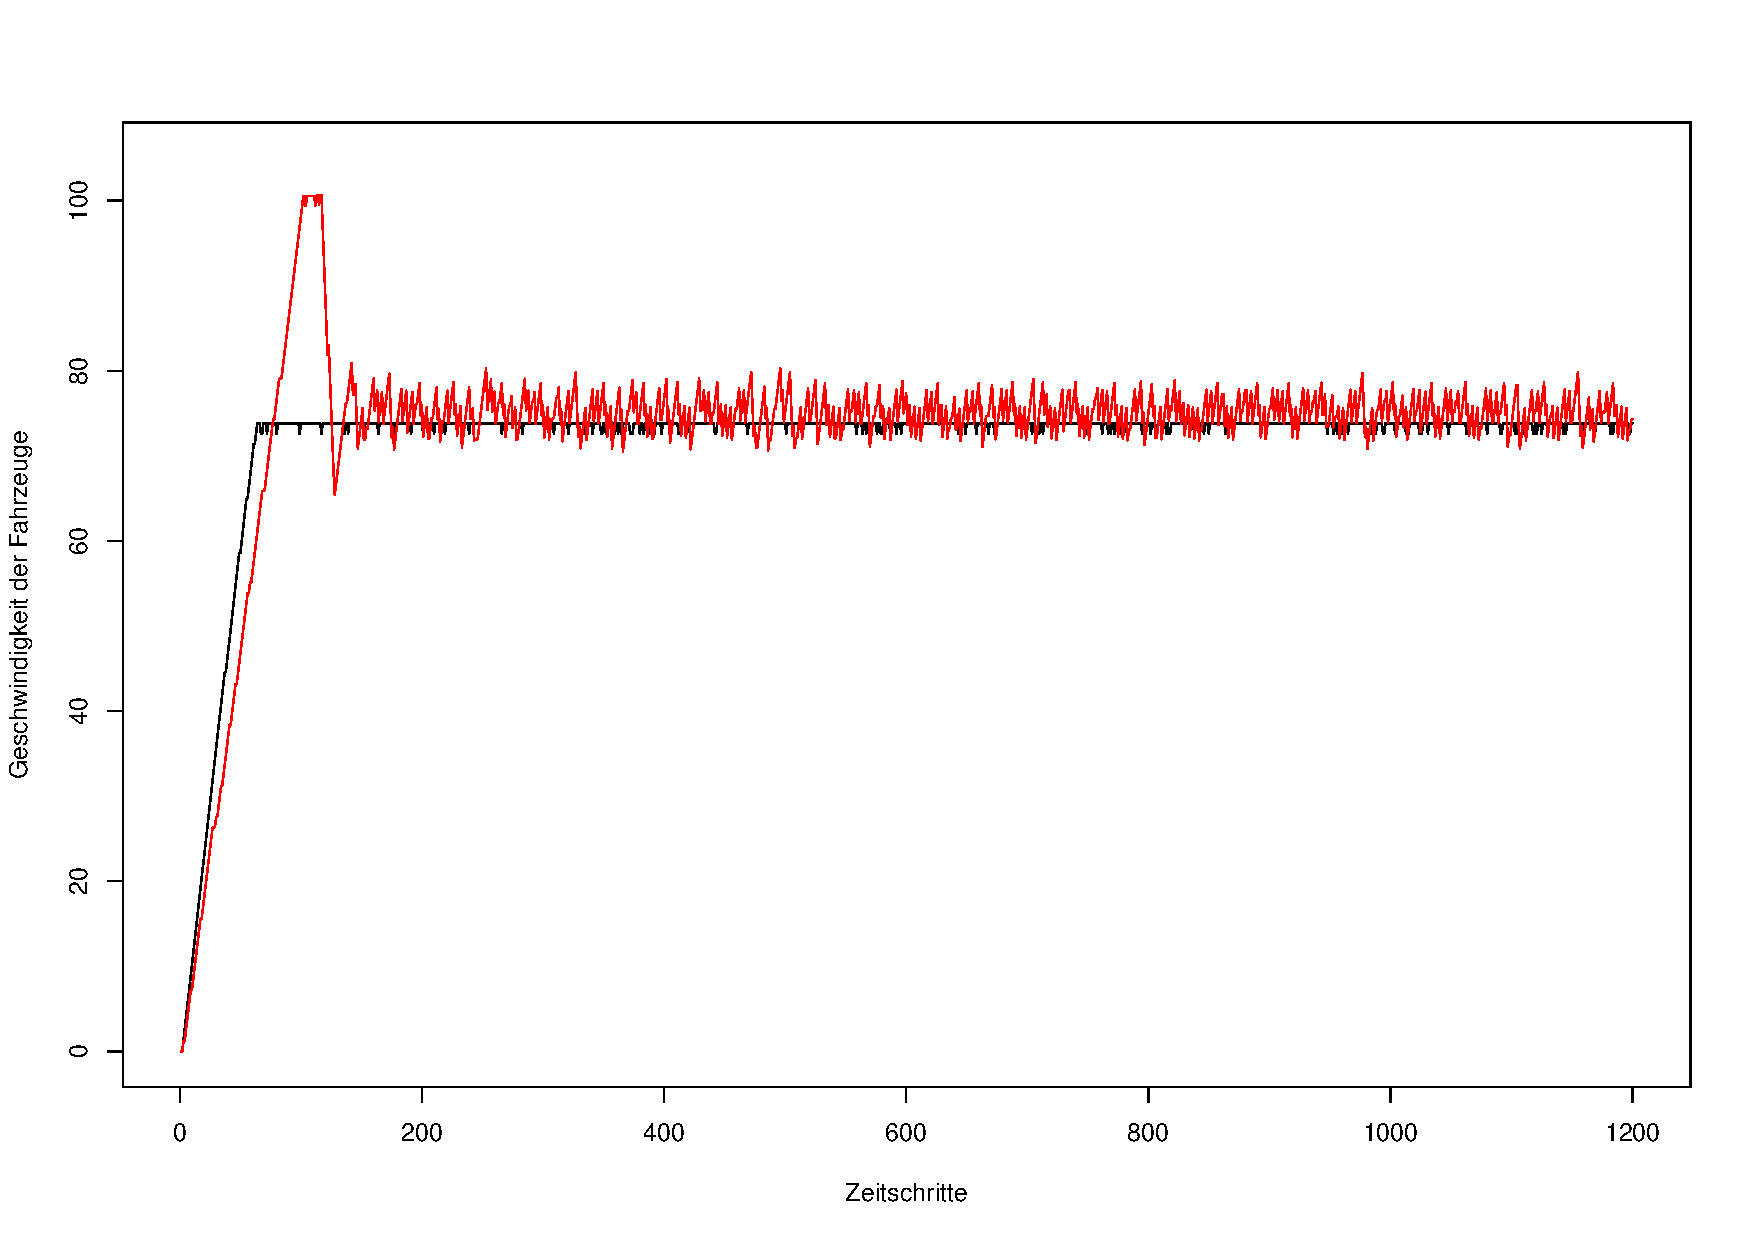
\includegraphics[width=0.45\textwidth]{speed_run27}\label{figure:testrun-34veh-7ko5km-position}}\qquad 
   \subfigure[Geschwindigkeiten]{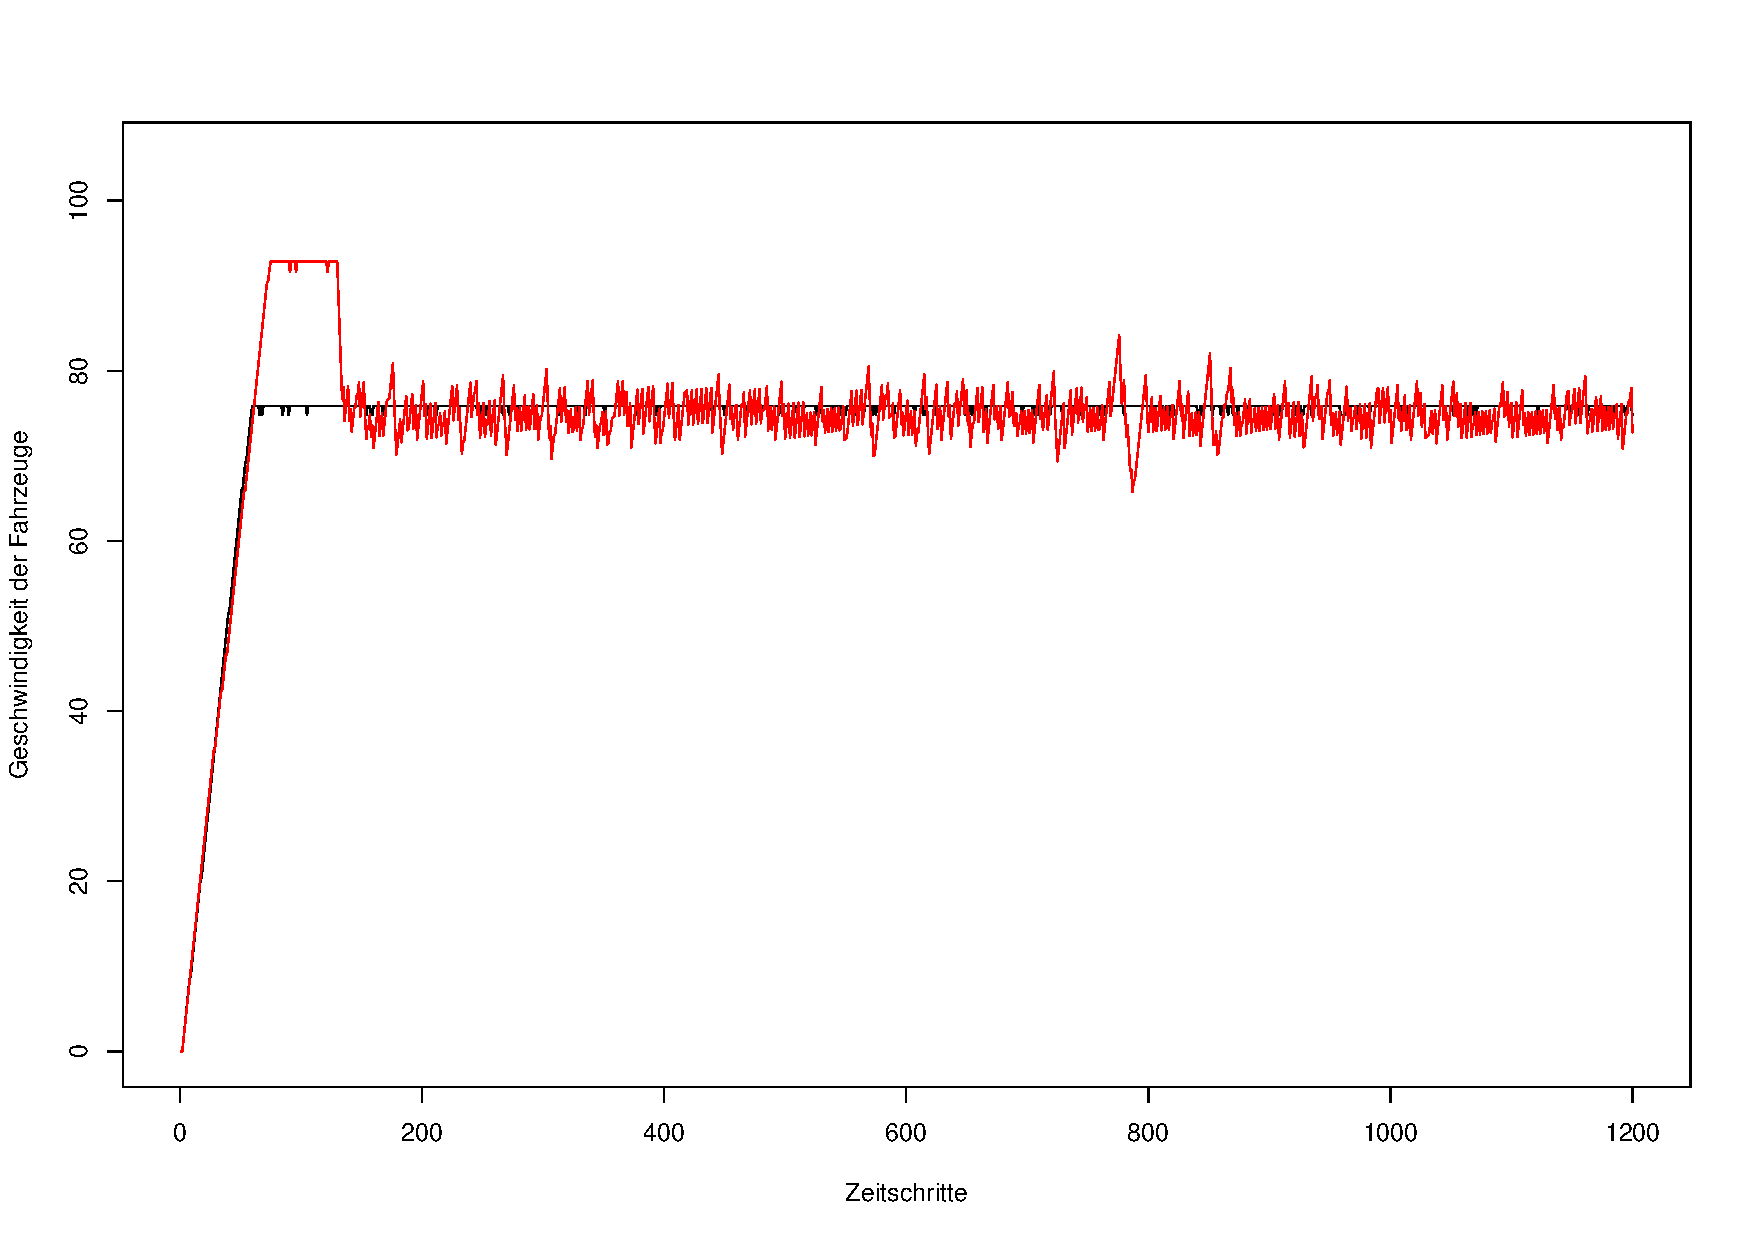
\includegraphics[width=0.45\textwidth]{speed_run28}\label{figure:testrun-34veh-7ko5km-speed}}
  \caption{Testlauf: 34 Fahrzeuge, 7,5 km Strecke, 2 Stunden} 
  \label{figure:testrun-34veh-7ko5km}
\end{figure}

\paragraph*{weitere Testläufe mit zunehmender Fahrzeuganzahl}

Es wurde weiterhin mit einstündigen Simulationen getestet, ab welcher Fahrzeuganzahl das Szenario ins Stocken gerät.
Es wurde festgestellt, dass dem Szenario noch \sa{own: add value} weitere Fahrzeuge hinzugefügt werden können, ohne den Verkehrsfluss deutlich zu beeinträchtigen.
Erst ab insgesamt \sa{own: add value} Fahrzeugen auf der Strecke bringen die Wechselwirkungen untereinander die entstehende Fahrzeugschlange zum Stoppen.




\subsubsection{Verkehrsmenge A38: 15 Fahrzeuge und Verkehrsmenge A71: 8 Fahrzeuge}
\label{sec:szenario-a38-a71}

\sa{own: content}
Da die Simulationsläufe in \cref{sec:szenario-a7} zeigten, dass die Strecke mit den gewählten Einstellungen mehr als das Doppelte, bzw. Vierfache an Verkehr verarbeiten konnte, waren aus den ausgeführten Durchläufen keine weiteren Erkenntnisse zu gewinnen.



\subsubsection{Beobachtungen}

Während bei der Entwicklung durchaus rückwärts laufende Stauwellen beobachtet werden konnten, siehe z.B. \cref{figure:33veh-1km}, ist die Phase der Totalstopps, die dieses Verhalten hervorruft, bei der Simulation des fließenden Verkehrs im allgemeinen nicht vorhanden.
\\
Dadurch dass die Bremsmanöver feiner ausgeführt werden, nähern sich die Positionen der Fahrzeuge einander an und fächern sich dann aber, nachdem die Ursache für das Abbremsen beseitigt ist, wieder auf.

In den Positionsplots bilden sich in den meisten Fällen weiße Streifen aus. Dies sind Stellen auf der Strecke, an denen sich kein Fahrzeug befindet.





\subsection{Erkenntnisse aus Entwicklung und Simulationsläufen}

Durch die einerseits real simulierten Beschleunigungs-, Verzögerungs- und Geschwindigkeitswerte, andererseits aber \enquote{grob} unterteilten Zellgrößen und Zeitabschnitte kommt es in der Simulation zu Verhalten, welches durch diese Unterschiede erklärbar ist.


\subsubsection{Zellgröße}

\paragraph{träges Anfahren:}
\label{sec:accelerategroove}

Aufgrund der vergleichbar zum NaSch-Modell gewählten Zellgröße von 7,5 Metern, im Gegensatz dazu aber die Simulation realitätsnaher Beschleunigungswerte, kommt es am Beginn des Simulationslaufs mehrere Zeitschritte lang zu einem Stillstand der Fahrzeuge.
Da jedes Fahrzeug softwareseitig in der Mitte der belegten Zelle platziert wird (bzw. im ersten Zeitschritt dorthin gesetzt wird) wird eine Geschwindigkeit von mehr als $ \frac{1}{2} \times $ 7,5 $ \frac{m}{s} = $ 13,5 km/h benötigt, um eine sichtbare Bewegung durchzuführen.
Durch die unterschiedliche Ausprägung der Beschleunigungswerte und möglicher Trödelphasen ist keine Nennung eines festen Zeitpunkts möglich, an dem dies vollzogen wird.

Im weiteren Verlauf der Simulation fällt es in der Weg-Zeit-Kurve nicht weiter auf, dass die Fahrzeuge an Zellen mit einer bestimmten Länge gebunden sind.



\paragraph{schlechte Bremswirkung:}
\label{sec:bremsverhalten}

Die Simulationsplattform bietet durch realistisch modellierte Beschleunigungen und Verzögerungen den Vorteil, dass der Verkehr feingranularer abgebildet werden kann.
Die analog zu den Simulationen von Nagel und Schreckenberg gewählte Zellgröße von 7,5 Metern führt allerdings dazu, dass theoretisch dargestellte Reduktionen der Geschwindigkeit nicht direkt in nächsten Zeitschritt umgesetzt werden.
Vielmehr muss, ähnlich wie beim soeben beschriebenen Anfahren, ein gewisser Wert unterschritten werden, damit die gezeigte Bewegung auch real kürzer gesetzt wird.

Reicht der Platz nach vorn nicht aus, um das Fahrzeug entsprechend seiner Geschwindigkeit zu bewegen und in die freie Zelle hinter das vorausfahrende Fahrzeug zu setzen, wird ein Kollisionsereignis ausgelöst.

Die Reaktion darauf kann über einen Agentenplan gesteuert werden.
Zu Beginn der Erarbeitung wurde die Kollision mit einem extremen Abbremsen modelliert, später dann als Totalstopp.
\\
Die Reduktion der Geschwindigkeit auf Null ist insofern vorteilhaft, weil der Extremausschlag nach unten im Plot der Geschwindigkeiten sichtbar ist.
Außerdem wird der Agent wirklich in der aktuellen Zelle gestoppt. 
Die Simulationsplattform würde sonst über (mehrere) Zeitschritte hinweg die Geschwindigkeit abbauen, ohne dass bedingt durch vorausliegende Hindernisse, eine reale Bewegung stattfinden könnte. 
\\
Nachteilig ist zu sehen, dass ein Totalstillstand aufgrund der großen Geschwindigkeitsunterschiede meist weitere Kollisionen nach sich zieht.

% --- Diese beiden Absätze sind gut - Phil FB 27feb
Die Schwierigkeiten beim Bremsen können durch Reduktion der Zellgröße bei ansonsten gleichen Voraussetzungen \enquote{behoben} werden.
Eine Simulation mit reduzierten Zellgrößen führte in diesem Aspekt zu einem harmonischeren Verkehrsbild.
Eine komplette Vermeidung der Kollisionsereignisse ist nicht gelungen, siehe auch nachfolgendes \cref{sec:mindestabstaende}.

Für die weitere Entwicklung könnte für die Fahrzeuge bei der Initialisierung eine Fahrzeuglänge generiert werden.
Dadurch würden diese mehrere dieser dann kleineren Zellen überdecken.
Dies hätte ein diversifizierteres Fahrzeugbild zur Folge und eröffnet die Möglichkeit präzisere Simulationen mit kleineren Zellen durchzuführen.
Zudem könnten Fahrzeugklassen auch in Sachen Platzbedarf realistisch dargestellt werden.


\subsubsection{Zeitschrittlänge}

\paragraph*{Worst Case-Analyse für Mindestabstände:}
\label{sec:mindestabstaende}

Das Kollisionsereignis wird nicht erst bei einer tatsächlichen Kollision, wenn sich zwei Fahrzeuge in einem Punkt treffen, ausgelöst, sondern bereits wenn der Platz nach vorn zum aktuellen Zeitpunkt nicht mehr zum Bewegen ausreichen würde.
Hierbei spielt es für das Simulationstool keine Rolle, dass das Hindernis in Bewegung ist und sich von dort entfernt.

Ein Verzögerungsvorgang - Abbremsen/Heranbremsen - muss also innerhalb einer kürzeren Strecke abgeschlossen werden, als dies in der Realität der Fall wäre.

In \cref{tab:restgeschw-abstand} sind die Mindestabstände für eine kollisionsfreie Bewegung für eine Zellgröße vom 2,5 m und einer Zeitschrittgröße von 0,025 und 0,05 min aufgeführt.
Zwischenschritte der Berechnung wurden jeweils aufgerundet.

\noindent
Anzahl zu setzender Zellen: $ x = \lceil \frac{\text{Geschwindigkeit}}{3,6} \times \frac{\text{Zeitschrittlänge}}{\text{Zellgröße}} \rceil $
\\
Mindestabstand: $ s_{min} = \lceil x \times \text{Zellgröße} \rceil $
\\
Fasste man beide Gleichungen zusammen, würde die Zellgröße aus der Gleichung entfernt.

\begin{table}[ht]
\begin{center}
\setlength{\tabcolsep}{0.5em} % for the horizontal padding
{\renewcommand{\arraystretch}{1.2}% for the vertical padding
\begin{tabular}{| c  c  c |}
\hline 
(Rest-) & $ s_{min} $ in m & $ s_{min} $ in m  \\ 
Geschwindigkeit & bei ts=0,025 min & bei ts=0,05 min \\ \hline 
130 & 55 & 110 \\ 
100 & 43 & 85 \\ 
80 & 35 & 68 \\ 
70 & 30 & 60 \\ 
60 & 25 & 50 \\ 
50 & 23 & 43 \\ 
30 & 13 & 25 \\ 
Schritt & 3 & 5 \\ \hline
\end{tabular}
}
\caption{Mindestabstände für Restgeschwindigkeit}
\label{tab:restgeschw-abstand}
\end{center}
\end{table}

Da die Zellgröße bei entsprechender Umstellung der obigen Gleichung keinerlei Einfluss auf die Berechnung hat, verändert eine Änderung des Wertes die Ergebnisse nicht grundlegend. 
Es wird lediglich auf ein Vielfaches der Zellgröße gerundet.
\\
Durch die Entfernungen, die in einem größeren Zeitschritt zurückgelegt werden, erhöht sich durch eine Anhebung der Zeitschrittlänge auch der Mindestabstand entsprechend.












%%.\sa{hier vermischst Du \cref{sec:sota} mit \cref{sec:realisierung}, hier geht es darum, wi Du konkret arbeiten willst um die Sachen unter \cref{sec:researchgap} zu beweisen oder zu belegen, evtl macht es Sinn diese Punkte mit in \cref{sec:sota} zu ziehen, Du kannst dann einfach, wenn Du es brauchst Verweise setzen}
%
%\noindent
%Die in \cite{dat-ba} vorgeschlagene Struktur ist zu implementieren und in vergleichbarer Umgebung simulatorisch zu testen. 
%Dabei sind die folgenden Größen zu erheben und entsprechend statistisch auszuwerten: 
%
%\begin{itemize}
%\item Verkehrsdichte
%\item Verkehrsfluss
%\item Spurwechselfrequenz
%\item Spurnutzung links/rechts
%\end{itemize}
%
%Das Testszenario wurde in \cite{na-sch} durch das zu Beginn zufällige Platzieren von Fahrzeugen in einem geschlossenen Kreis mit $L$ Zellen (ähnlich einer Autorennstrecke) simuliert. \\
%Allerdings wurde auch, bei der Simulation einer Fahrbahnverengung, eine Alternative Simulationsmöglichkeit beschrieben. 
%Eine Gridgerade von bis zu 10000 Zellen Länge wurde getestet - Bewegungsrichtung von links nach rechts. 
%Die Fahrzeuge wurden mit $v=0$ in die am weitesten links befindliche Zelle, so diese frei war, gesetzt und die Fahrzeuge in den sechs am weitesten rechts befindlichen Zellen (bei systemweiter $v_{max}=5$) gelöscht. 
%Letzteres Vorgehen sorgte für eine offene Grenze für den abfließenden Verkehr.
%
%Für eine kontinuierliche Simulation ist die zweite Möglichkeit ungeeignet. 
%Auch in \cite{multi-lane} wird von der Nutzung periodischer Randbedingungen gesprochen. 
%Dies lässt darauf schließen, dass, wie in \cite[Abb. 1.5]{peri-rand} für die Umgebung von Pixeln beschrieben, die Fahrzeuge vom \enquote*{Ende} der Gridstrecke am \enquote*{Anfang} wieder eingesetzt wurden und somit der zuerst beschriebene Kreis einsteht.
%Dieses Verhalten ist zu bevorzugen.
%
%Vorteil der geschlossenen Kreisstrecke ist, dass man bei konstanter Fahrzeuganzahl $N$ (bei \cite{multi-lane} waren dies $N = 10^{3}$) durch die Veränderung der Systemgröße eine unterschiedliche Fahrzeugdichte erreicht werden kann. 
%Jeder Dichtewert wurde für $T = 10^{5}$ Zeitschritte simuliert, wobei die erste Hälfte verworfen wurde, um mögliche Störeffekte ausklingen zu lassen. 
%Die generierten Simulationsdaten wurden über $T_{sample} = 300$ Zeitschritte und eine Wegstrecke von 133 Zellen, was etwa 1 km Länge in der realen Welt entspricht, gemittelt, um statistische Schwankungen zu reduzieren.
%
%Ein mögliches Simulationstool ist das \enquote{Traffic Simulation Game}\footnote{\link{https://lightjason.github.io/news/2017-09-workshop/}}. 
%In der Grundkonfiguration erzeugt dieses eine beliebig lange, gerade Straße mit beliebig vielen Fahrspuren. 
%ſEs ist zu prüfen, ob die Software auf die gewünschte Verhaltensweise angepasst werden kann.
